\documentclass[]{article}
\usepackage{lmodern}
\usepackage{amssymb,amsmath}
\usepackage{ifxetex,ifluatex}
\usepackage{fixltx2e} % provides \textsubscript
\ifnum 0\ifxetex 1\fi\ifluatex 1\fi=0 % if pdftex
  \usepackage[T1]{fontenc}
  \usepackage[utf8]{inputenc}
\else % if luatex or xelatex
  \ifxetex
    \usepackage{mathspec}
  \else
    \usepackage{fontspec}
  \fi
  \defaultfontfeatures{Ligatures=TeX,Scale=MatchLowercase}
\fi
% use upquote if available, for straight quotes in verbatim environments
\IfFileExists{upquote.sty}{\usepackage{upquote}}{}
% use microtype if available
\IfFileExists{microtype.sty}{%
\usepackage{microtype}
\UseMicrotypeSet[protrusion]{basicmath} % disable protrusion for tt fonts
}{}
\usepackage[margin=1in]{geometry}
\usepackage{hyperref}
\hypersetup{unicode=true,
            pdftitle={Oregon Extended Analyses: 2018},
            pdfauthor={Brock Rowley; Daniel Anderson; Sevrina Tindal; Gerald Tindal},
            pdfborder={0 0 0},
            breaklinks=true}
\urlstyle{same}  % don't use monospace font for urls
\usepackage{longtable,booktabs}
\usepackage{graphicx,grffile}
\makeatletter
\def\maxwidth{\ifdim\Gin@nat@width>\linewidth\linewidth\else\Gin@nat@width\fi}
\def\maxheight{\ifdim\Gin@nat@height>\textheight\textheight\else\Gin@nat@height\fi}
\makeatother
% Scale images if necessary, so that they will not overflow the page
% margins by default, and it is still possible to overwrite the defaults
% using explicit options in \includegraphics[width, height, ...]{}
\setkeys{Gin}{width=\maxwidth,height=\maxheight,keepaspectratio}
\IfFileExists{parskip.sty}{%
\usepackage{parskip}
}{% else
\setlength{\parindent}{0pt}
\setlength{\parskip}{6pt plus 2pt minus 1pt}
}
\setlength{\emergencystretch}{3em}  % prevent overfull lines
\providecommand{\tightlist}{%
  \setlength{\itemsep}{0pt}\setlength{\parskip}{0pt}}
\setcounter{secnumdepth}{0}
% Redefines (sub)paragraphs to behave more like sections
\ifx\paragraph\undefined\else
\let\oldparagraph\paragraph
\renewcommand{\paragraph}[1]{\oldparagraph{#1}\mbox{}}
\fi
\ifx\subparagraph\undefined\else
\let\oldsubparagraph\subparagraph
\renewcommand{\subparagraph}[1]{\oldsubparagraph{#1}\mbox{}}
\fi

%%% Use protect on footnotes to avoid problems with footnotes in titles
\let\rmarkdownfootnote\footnote%
\def\footnote{\protect\rmarkdownfootnote}

%%% Change title format to be more compact
\usepackage{titling}

% Create subtitle command for use in maketitle
\newcommand{\subtitle}[1]{
  \posttitle{
    \begin{center}\large#1\end{center}
    }
}

\setlength{\droptitle}{-2em}

  \title{Oregon Extended Analyses: 2018}
    \pretitle{\vspace{\droptitle}\centering\huge}
  \posttitle{\par}
    \author{Brock Rowley \\ Daniel Anderson \\ Sevrina Tindal \\ Gerald Tindal}
    \preauthor{\centering\large\emph}
  \postauthor{\par}
      \predate{\centering\large\emph}
  \postdate{\par}
    \date{6/29/2018}

\usepackage{booktabs}
\usepackage{longtable}
\usepackage{array}
\usepackage{multirow}
\usepackage[table]{xcolor}
\usepackage{wrapfig}
\usepackage{float}
\usepackage{colortbl}
\usepackage{pdflscape}
\usepackage{tabu}
\usepackage{threeparttable}
\usepackage{threeparttablex}
\usepackage[normalem]{ulem}
\usepackage{makecell}

\usepackage{placeins}
\usepackage{float}
\usepackage{caption}
\captionsetup[figure]{labelformat = empty}
\usepackage{xcolor}
\definecolor{link}{rgb}{0, 0, 238}
\usepackage{booktabs}

\begin{document}
\maketitle

{
\setcounter{tocdepth}{4}
\tableofcontents
}
\newpage

\begin{figure}
\centering

\includegraphics{img/stateofOR.png}
\caption{}
\end{figure}

\section{Oregon Department of
Education}\label{oregon-department-of-education}

\section{2017-2018 Technical Report}\label{technical-report}

\subsection{Oregon's Alternate Assessment
System}\label{oregons-alternate-assessment-system}

\subsection{Peer Review Documentation: Critical Elements
1-6}\label{peer-review-documentation-critical-elements-1-6}

\subsubsection{Oregon's Alternate Assessment System Technical
Report:}\label{oregons-alternate-assessment-system-technical-report}

\subsubsection{Peer Review Documentation: Critical Elements
1-6}\label{peer-review-documentation-critical-elements-1-6-1}

It is the policy of the State Board of Education and a priority of the
Oregon Department of Education that there will be no discrimination or
harassment on the grounds of race, color, religion, sex, sexual
orientation, national origin, age or disability in any educational
programs, activities or employment. Persons having questions about equal
opportunity and nondiscrimination should contact the Deputy
Superintendent of Public Instruction with the Oregon Department of
Education.

\emph{This technical report is one of a series that describes the
development of Oregon's Statewide Assessment System. The complete set of
volumes provides comprehensive documentation of the development,
procedures, technical adequacy, and results of the system.}

\newpage

\begin{figure}
\centering
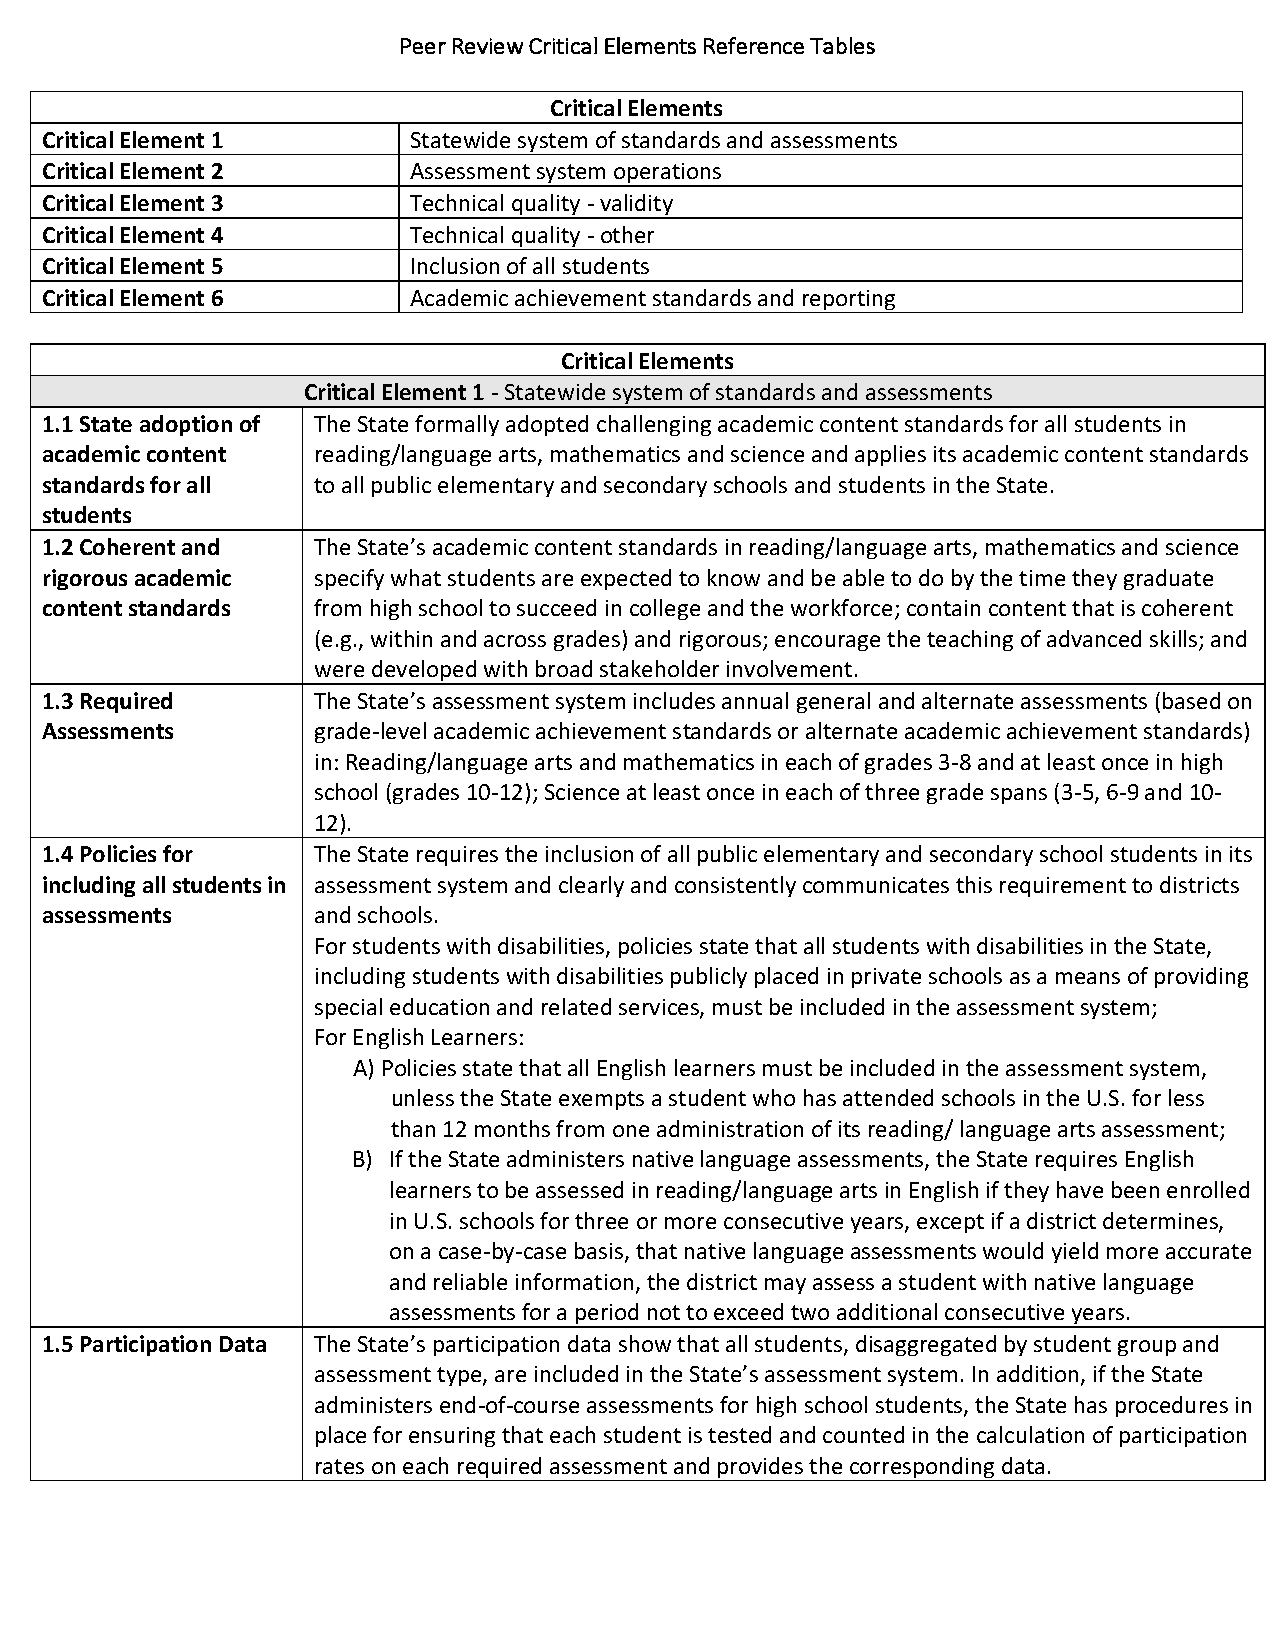
\includegraphics{Figures/peer_rev/PeerReview1.pdf}
\caption{}
\end{figure}

\newpage

\begin{figure}
\centering
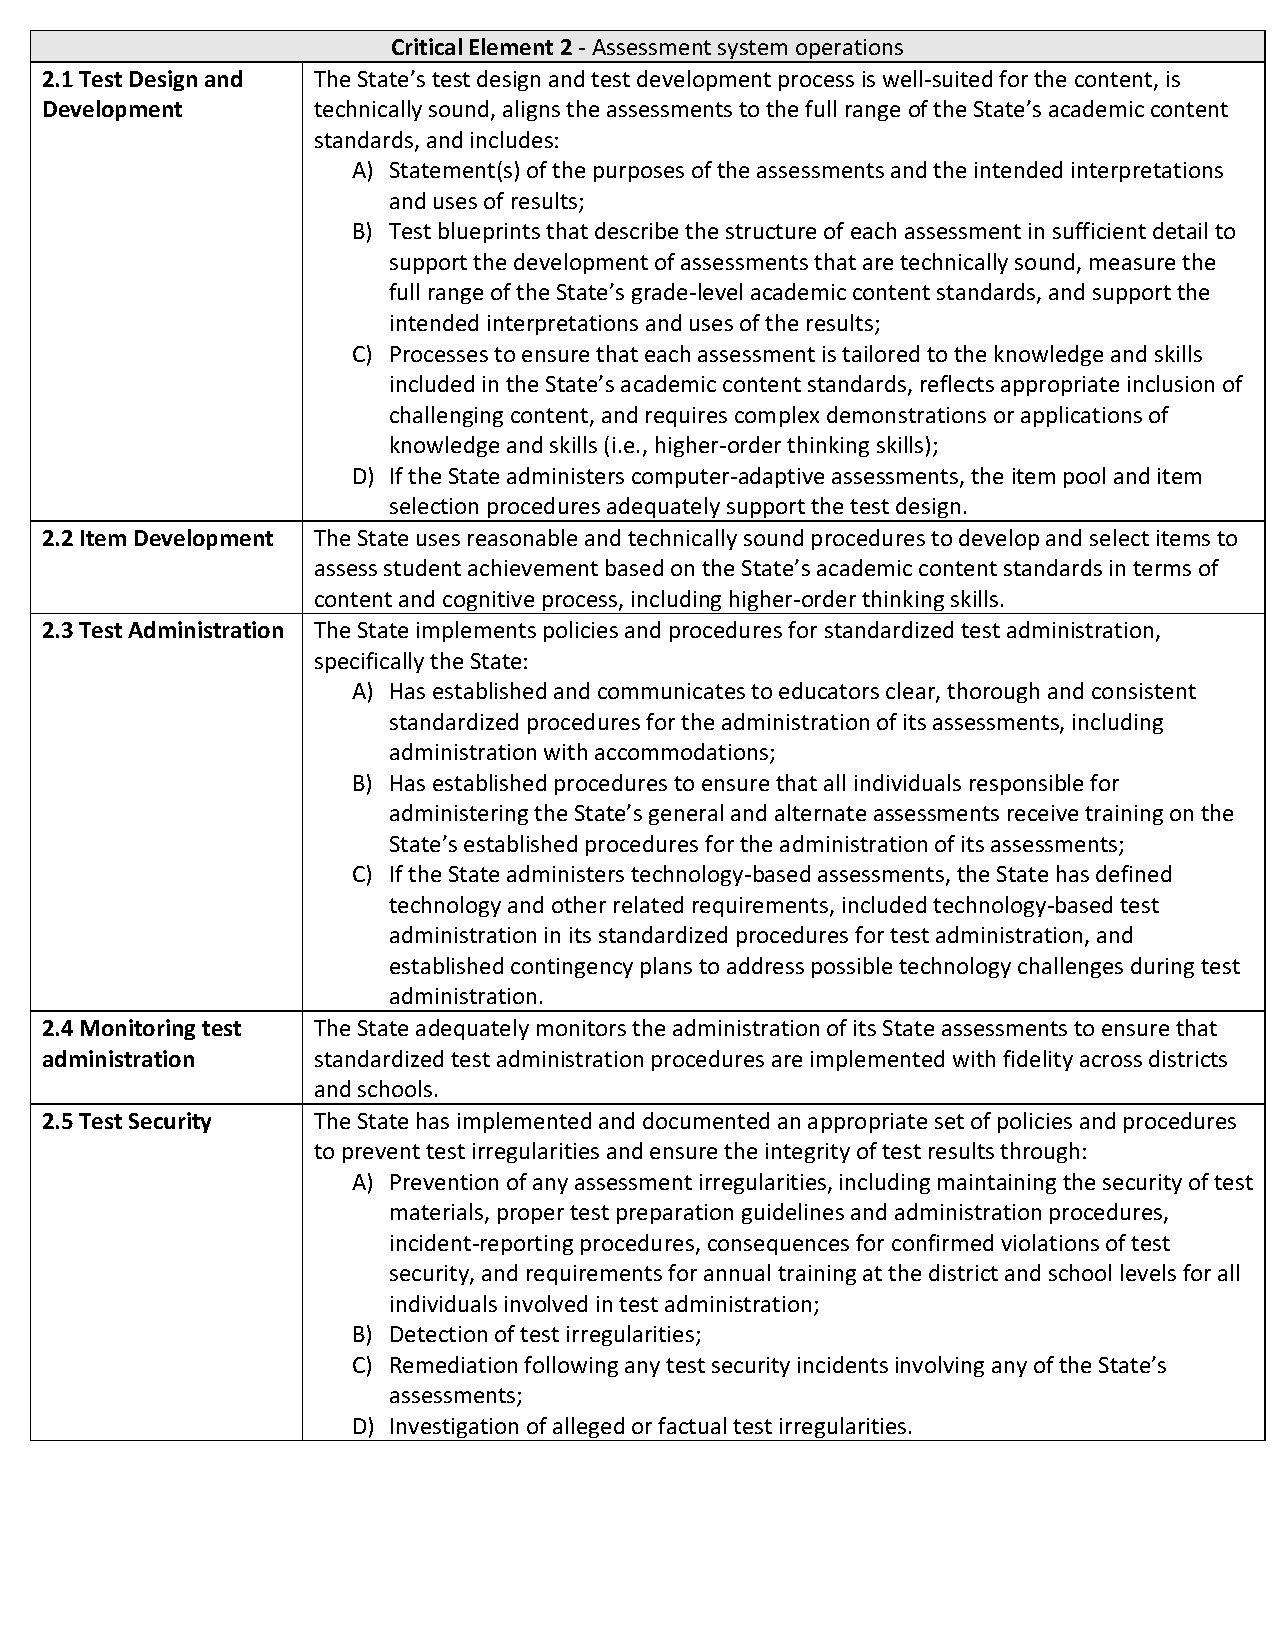
\includegraphics{Figures/peer_rev/PeerReview2.pdf}
\caption{}
\end{figure}

\newpage

\begin{figure}
\centering
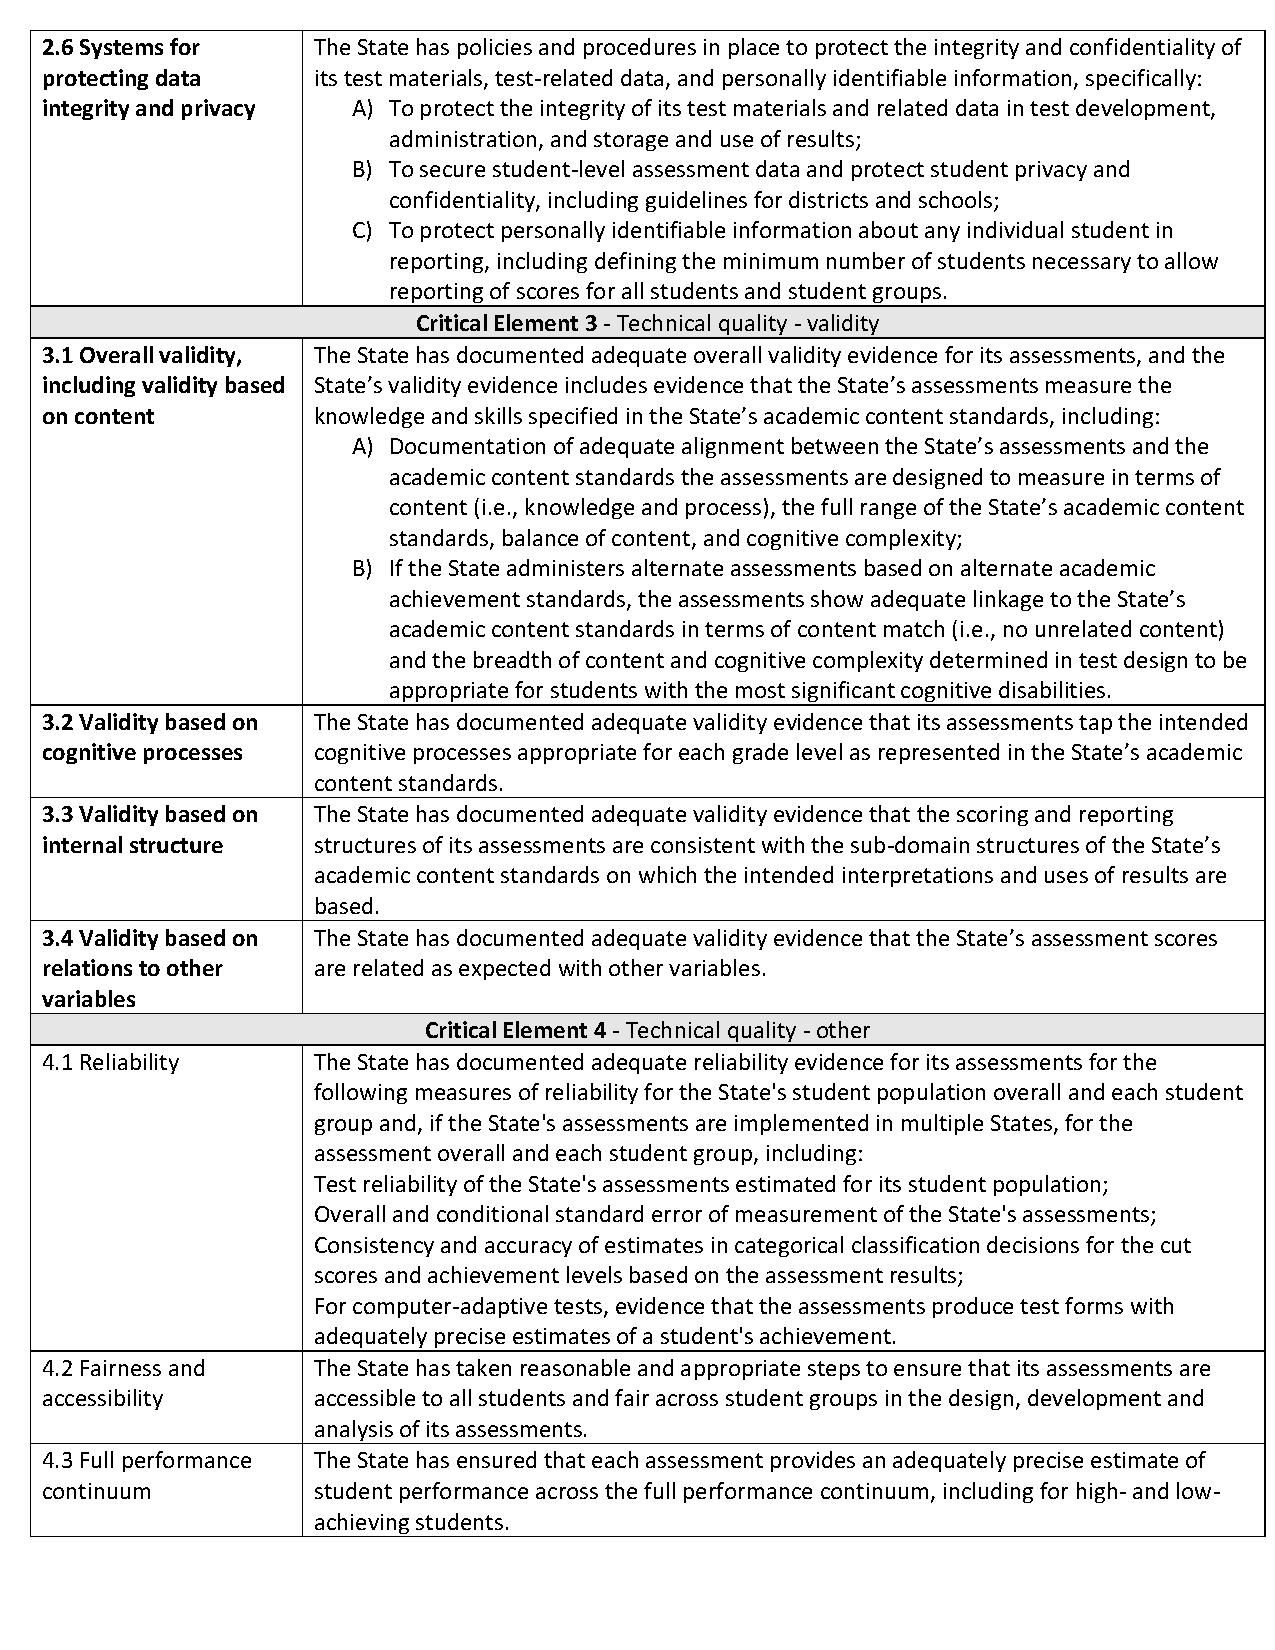
\includegraphics{Figures/peer_rev/PeerReview3.pdf}
\caption{}
\end{figure}

\newpage

\begin{figure}
\centering
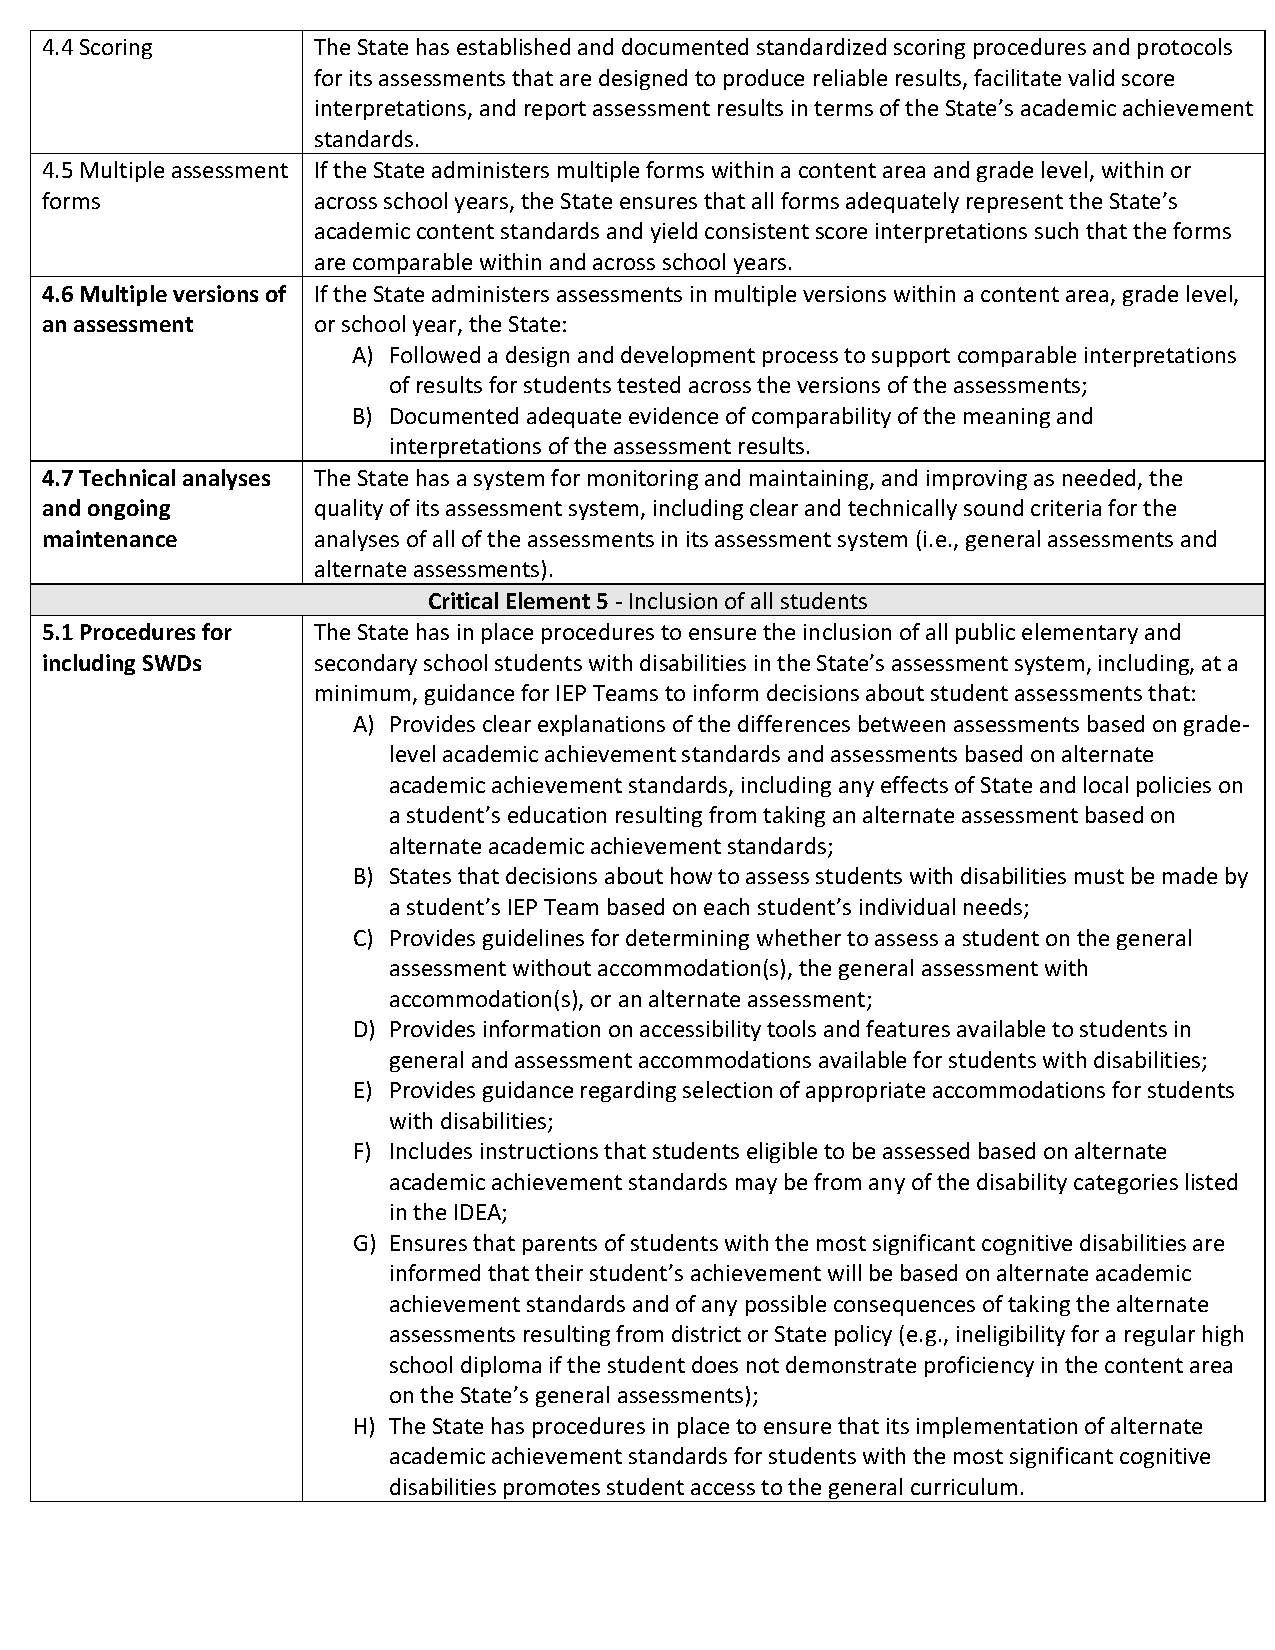
\includegraphics{Figures/peer_rev/PeerReview4.pdf}
\caption{}
\end{figure}

\newpage

\begin{figure}
\centering
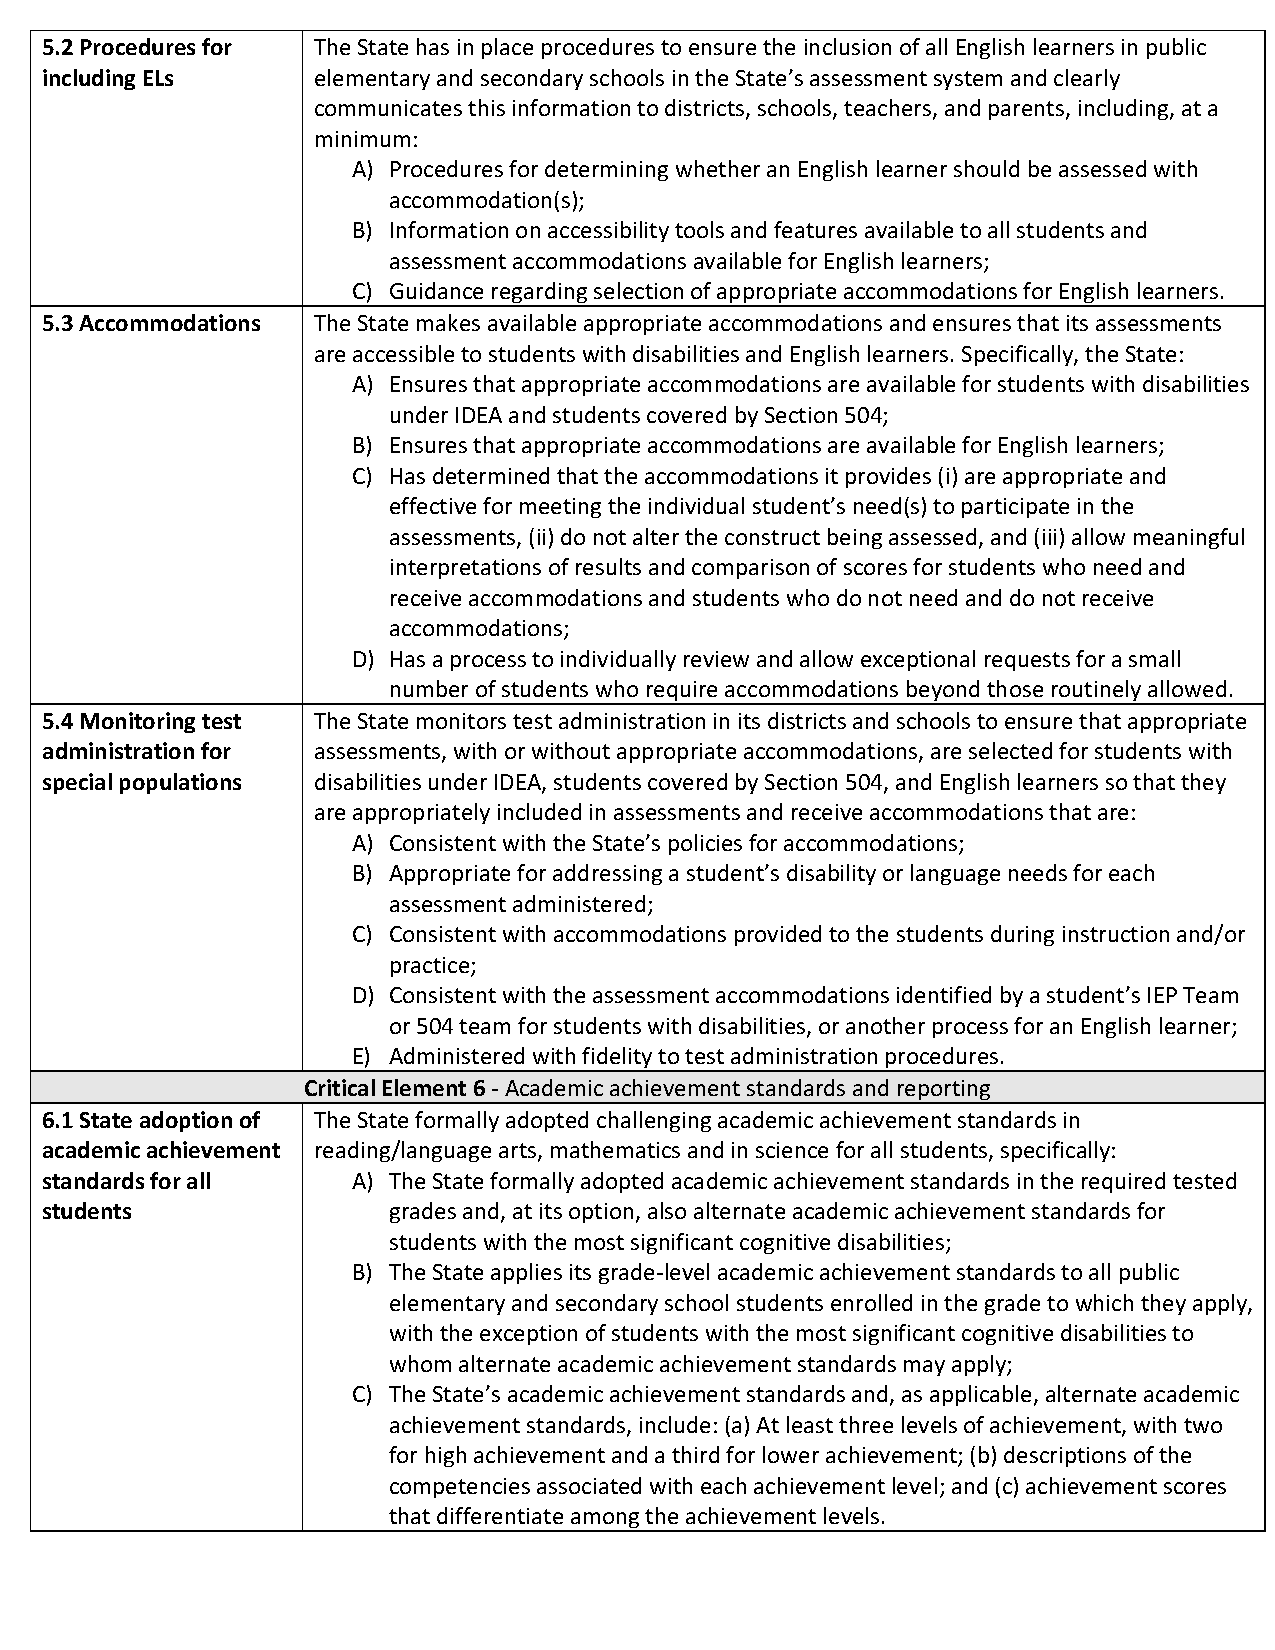
\includegraphics{Figures/peer_rev/PeerReview5.pdf}
\caption{}
\end{figure}

\newpage

\begin{figure}
\centering
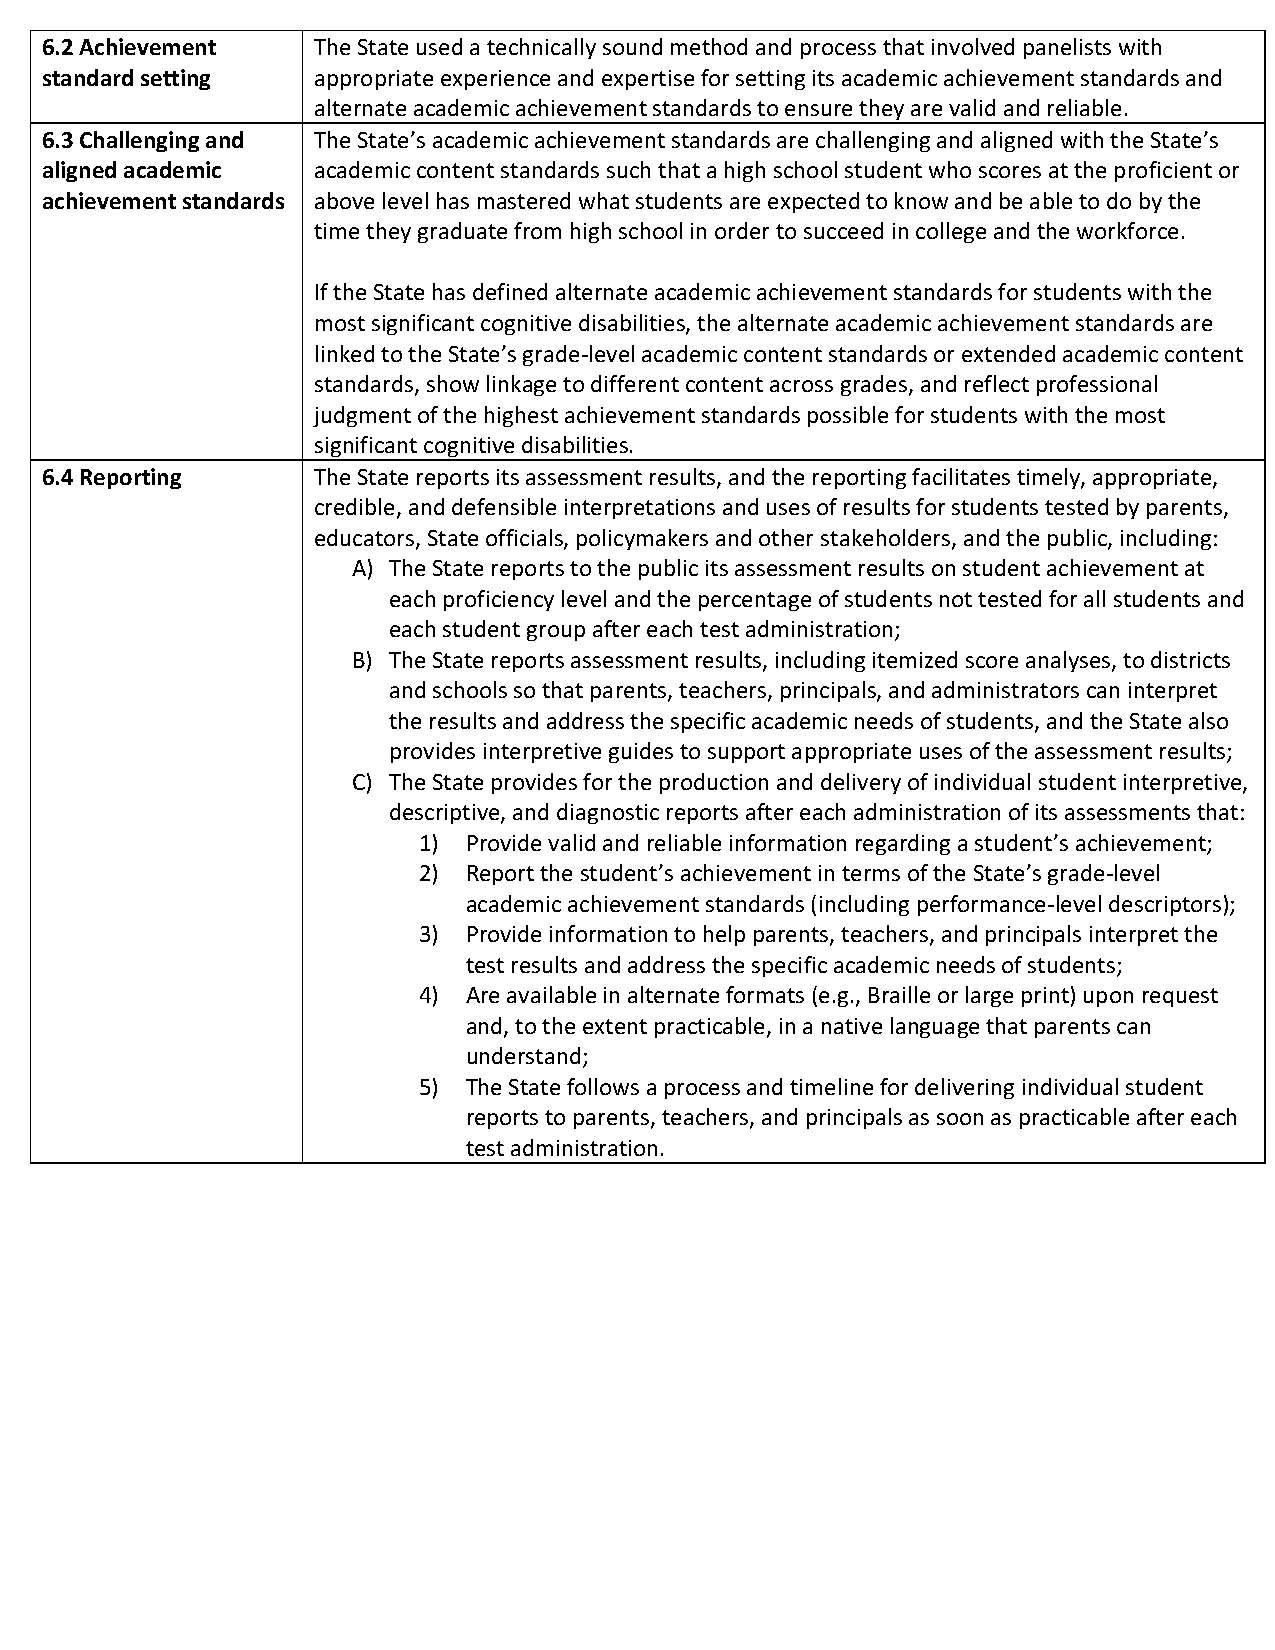
\includegraphics{Figures/peer_rev/PeerReview6.pdf}
\caption{}
\end{figure}

\section{Overview}\label{overview}

This document provides updated technical adequacy documentation for the
Oregon Extended Assessment (ORExt), which is Oregon's alternate
assessment based on alternate academic achievement standards (AA-AAAS).
The documentation includes test design and development, technical
characteristics of the assessments, and their uses, and impact in
providing proficiency data on grade level state standards as part of the
mandates from the Every Student Succeeds Act of 2015 (ESSA).

The ORExt assessments were redesigned in 2014-15, including a vertical
scale in Grades 3-8 in English language arts and mathematics to support
eventual determinations of student growth over time. The test is aligned
to Essentialized Standards (EsSt) that are part of comprehensive
Essentialized Assessment Frameworks (EAFs) that were written at three
levels of complexity (low, medium, and high). The EsSt have been linked
to grade level content and expectations, but systematically reduced in
terms of depth, breadth, and complexity (RDBC). All ORExt items employed
in the 2017-18 ORExt administration, with the exception of Grade 7 Math
field test items, were developed in 2014-15. Based on student
performance from the 2016-2017 testing year, new and Grade 7 Math field
test items were written in fall 2017.

A statewide sample of Oregon general and special education teachers have
reviewed all test items for: 1) alignment to the EAFs, 2) accessibility
for students with significant cognitive disabilities, 3) sensitivity,
and 4) bias. All operational items met the established criteria. In
addition, Achievement Level Descriptors (ALDs) were also reviewed for
alignment to the EsSt. See Sections 1.1, 1.2, 6.1, and 6.3 for
additional information related to the comprehensive grade level
standards to EsSt linkage, as well as alignment of items to the EsSt.

The ORExt test design supports student access, including access to read
aloud for directions and prompts, presentation of one item per page, and
items designed at three levels of complexity where the low level
complexity items include graphic and/or object support. For assessors,
the scoring process has also been simplified, with answers being either
correct (1) or incorrect (0). Partial credit is no longer part of the
scoring metric for the ORExt. In addition, the one item per page format
not only increases student ability to focus attention, but also reduces
the burden on assessors to mask items that are not being tested. The
field appears to have been appreciative of the redesign, particularly
the Essentialized Standards and new access and efficiency features.

In addition to developing and reviewing/editing over 5,000 new items,
conducting an operational field test, and developing a vertical scale,
the development of a new ORExt required that new Alternate Academic
Achievement Standards (AAAAS) be developed and approved. Comprehensive
Standard Setting meetings were conducted on June 15-17, 2015, which were
then approved by the Oregon State Board of Education on June 25, 2015,
including new achievement level descriptors (ALDs) and cut scores for
the assessments. Comprehensive Annual Measurable Objective (AMO) reports
were finalized on July 10, 2015.

Though an alignment study was conducted in the fall of 2014 as described
above, Non-Regulatory Guidance from the U.S. Department of Education,
published on September 25, 2015, included an expectation that all
alignment studies must be independent (see Critical Element 3.1). An
independent contractor, Dr.~Dianna Carrizales, was therefore hired to
perform an additional alignment study in the spring of 2017.

A two year pilot tablet study was conducted in the 2015-2016 and 2016-17
school years. Over the two year study, 26 students were administered all
subject areas of the ORExt in tablet format in grades 5, 8, and 11. The
2017-18 school year marked the first year the ORExt was available in
tablet/online format for all grades in all subject areas.

As part of our five-year technical documentation plan, which included
the independent alignment study, pilot tablet administration study, and
launch of the full tablet administration, an inter-rater reliability
study was also conducted in 2017-18. The inter-rater reliability study
included 33 Qualified Trainers from around the state who participated by
doing at least one Qualified Assessor observation on the Oregon Extended
Assessment via paper/pencil administration. Included in the future of
the five-year plan is continuation of the inter-rater reliability study,
and analyses of the impact of accommodations.

\subsection{Critical Element 1: Statewide System of Standards and
Assessments}\label{critical-element-1-statewide-system-of-standards-and-assessments}

\subsubsection{1.1 State Adoption of Academic Content Standards for All
Students}\label{state-adoption-of-academic-content-standards-for-all-students}

The Oregon State Board of Education (SBE) adopted new, challenging
academic content standards, the
\color{link}\href{https://www.oregon.gov/ode/educator-resources/standards/Pages/default.aspx}{Common
Core State Standards (CCSS)}\color{black}, in English language arts and
mathematics in Grades K-12 on October 28, 2010. These CCSS are utilized
for all students in Oregon's public schools. Oregon was actively
involved in the development of the CCSS, as the Oregon Department of
Education (ODE), the Educational Enterprise Steering Committee (EESC),
Oregon's Education Service Districts, and school district
representatives provided feedback on the draft CCSS standards.

Similarly, the SBE adopted the
\color{link}\href{https://www.oregon.gov/ode/educator-resources/standards/science/Pages/Science-Standards.aspx}{Next
Generation Science Standards (NGSS)} \color{black} on March 6, 2014. The
NGSS establish learning targets for all students in Oregon's public
schools in Grades K-12. The ODE and the Oregon Science Content and
Assessment Panel provided direct feedback related to the NGSS. The NGSS
are being phased in over time instructionally, so students are being
assessed relative to the Oregon Science (ORSci) standards that were
adopted in 2009.

The newly adopted academic content standards were then reduced in depth,
breadth, and complexity through a process called essentialization. The
new
\color{link}\href{http://www.brtprojects.org/publications/training-modules}{Essentialized
Assessment Frameworks (EAFs)} \color{black} were then used for item
writing for the ORExt. The tables below provide examples of
essentialized standards in grades 5, 8, \& 11 in the subject areas of
English language arts (ELA), mathematics, and science. In the right
column are designations for estimated difficulty of an item: L (low), M
(medium), and H (high). More information on the essentialization process
can be found in section 1.2.

See \emph{Appendix} 1.1 for a User Guide that explains the development
process and intended uses for the EAFs.

\FloatBarrier
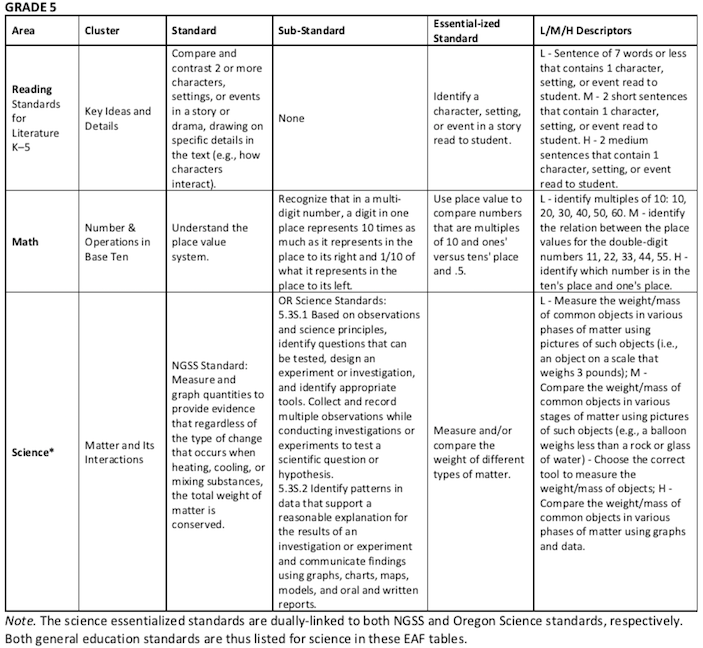
\includegraphics{Figures/Standards/Grade5.png}

\begin{figure}
\centering
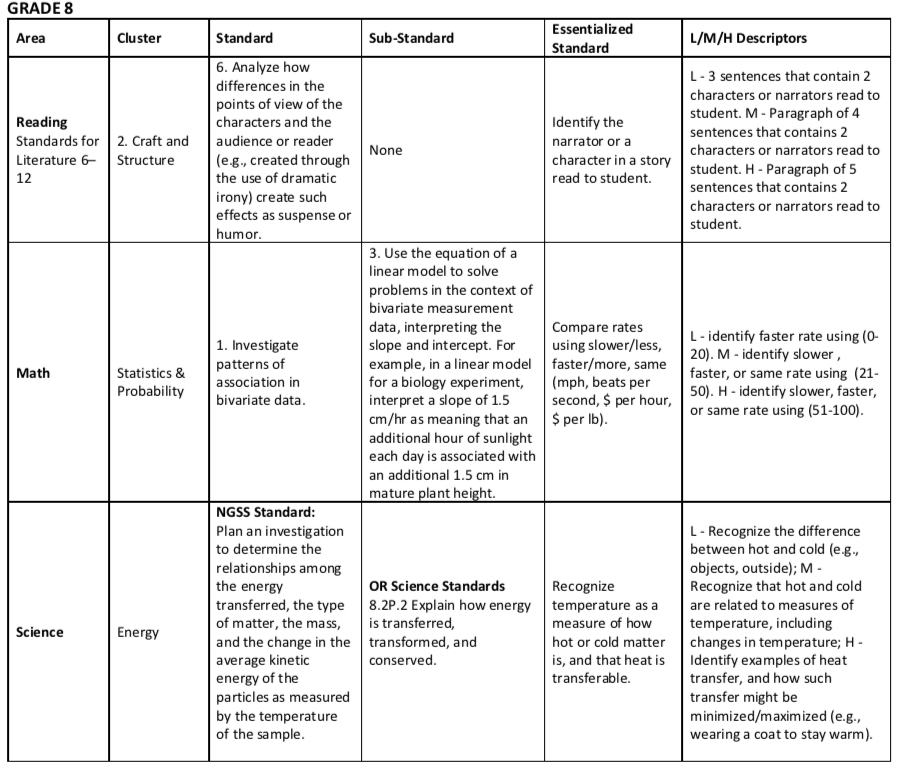
\includegraphics{Figures/Standards/Grade8.png}
\caption{}
\end{figure}

\begin{figure}
\centering
\includegraphics{Figures/Standards/Grade11.pdf}
\caption{}
\end{figure}

\clearpage

\subsubsection{1.2 Coherent and rigorous Academic Content
Standards}\label{coherent-and-rigorous-academic-content-standards}

The CCSS, ORSci, and NGSS define what students in Oregon should know and
be able to do by the time they graduate from high school. These CCSS,
which were developed by national stakeholders and education experts,
have been determined to be coherent and rigorous by researchers at the
Fordham Institute (see \emph{Appendix} 1.2). They were also developed
with wide stakeholder involvement, particularly here in Oregon. The new
ORExt is linked directly to the content in the CCSS in English language
arts (reading, writing, \& language) and mathematics. The ORExt is
dually linked to the ORSci as well as the NGSS. The NGSS are widely
accepted by most relevant science instruction organizations as
reflective of rigorous and coherent science concepts.

The new Essentialized Assessment Frameworks (EAFs) are publicly
available. A User Guide is provided to instruct educators regarding the
intended uses of the Essentialized Standards (EsSt), including the
development of Present Levels of Academic Achievement and Functional
Performance (PLAAFP) and Individualized Education Program (IEP) goals
and objectives. The basic essentialization process employed to generate
essentialized standards and write aligned items for the ORExt is
outlined below. The process can also be used to support the development
of curricular and instructional materials, founded in research-based
pedagogy. \FloatBarrier
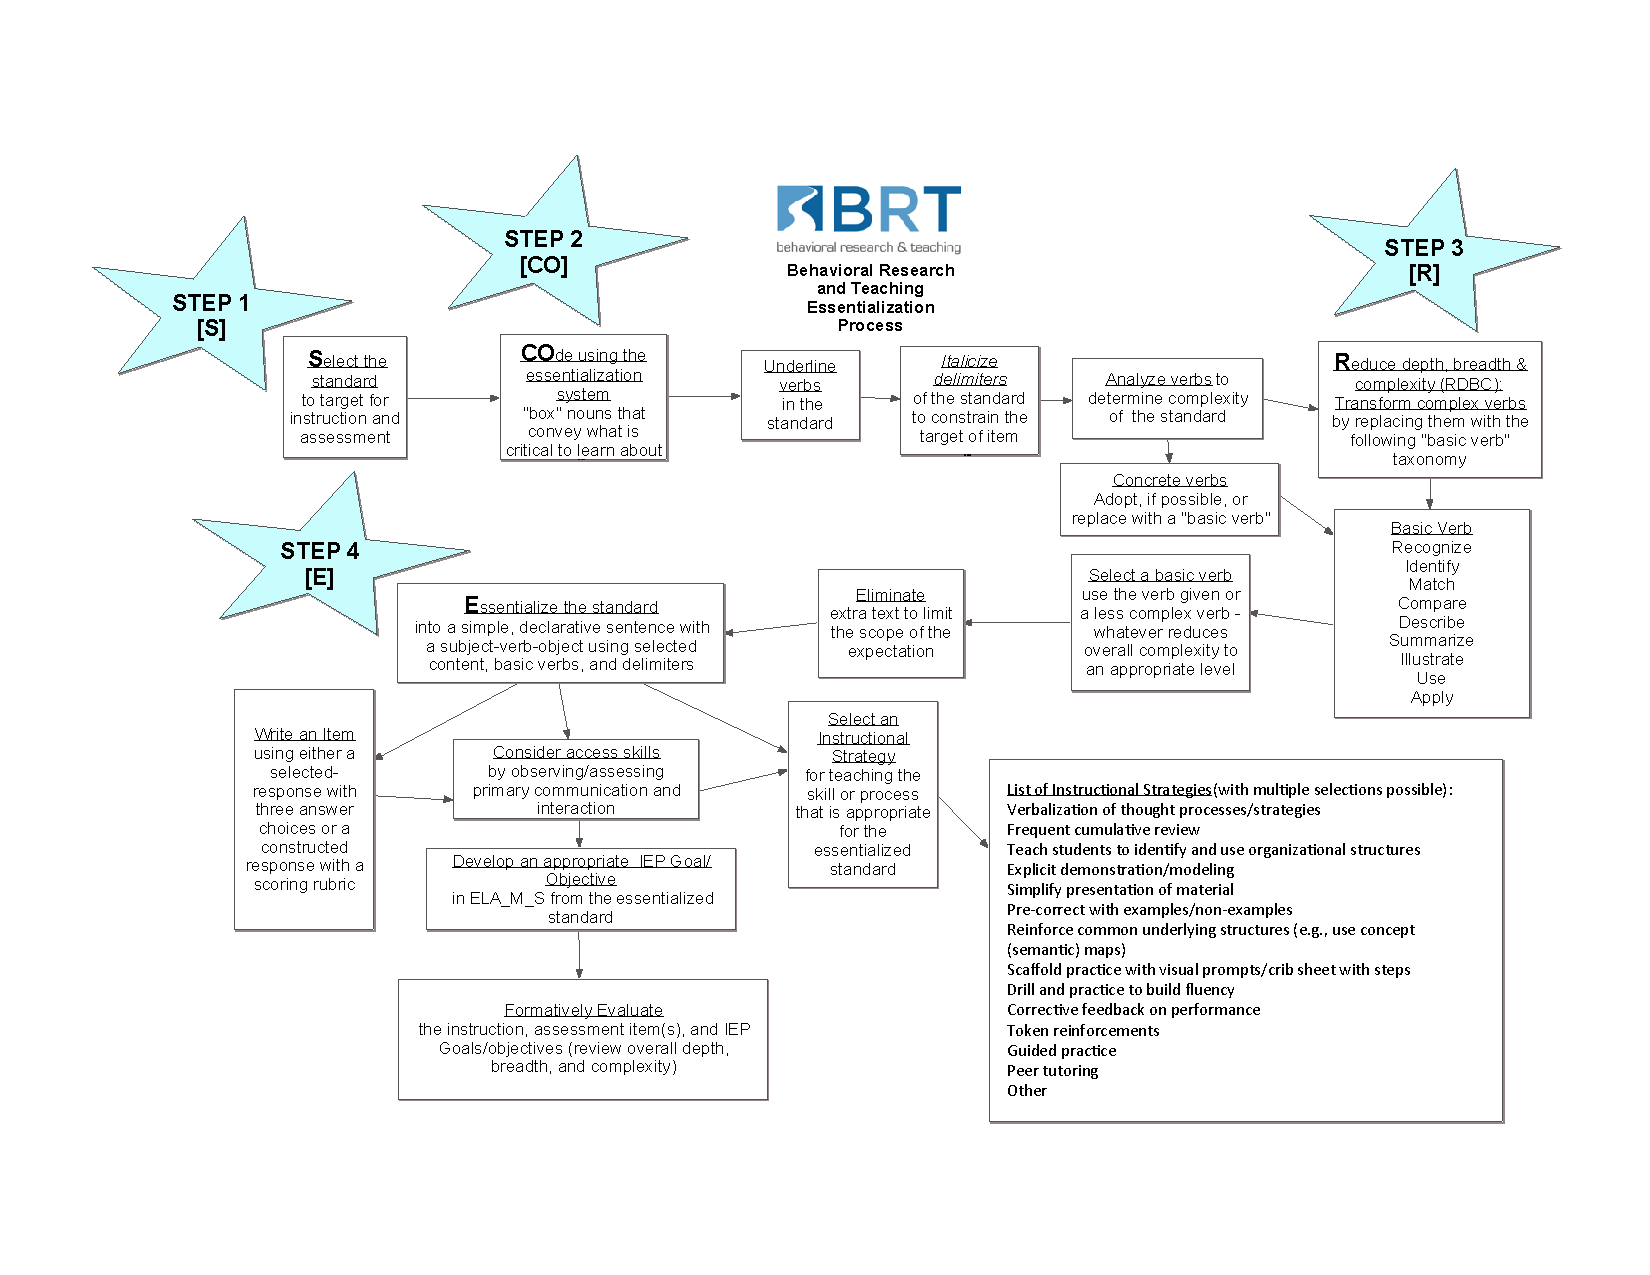
\includegraphics{Figures/Essentialization/Essentialization.pdf} \newpage

\subsubsection{1.3 Required Assessments}\label{required-assessments}

The ORExt assessments were administered in the 2017-18 school year in
ELA and math in Grades 3-8 and Grade 11; science is assessed in Grades
5, 8, \& 11. This assessment plan meets the requirements for grade level
assessment in Grades 3-8 and once in high school (Grades 10-12) for ELA
and mathematics, while science is assessed once in the 3-5 grade band,
once in the 6-9 grade band, and once in the 10-12 grade band:

\begin{longtable}[]{@{}lllllll@{}}
\toprule
\textbf{Content Area} & \textbf{Grade 3} & \textbf{Grade 4} &
\textbf{Grade 5} & \textbf{Grade 7} & \textbf{Grade 8} & \textbf{Grade
11}\tabularnewline
\midrule
\endhead
English Language Arts & X & X & X & X & X & X\tabularnewline
Mathematics & X & X & X & X & X & X\tabularnewline
Science & & & X & & X & X\tabularnewline
\bottomrule
\end{longtable}

\subsubsection{1.4 Policies for Including All Students in
Assessments}\label{policies-for-including-all-students-in-assessments}

Originally, Oregon statute required that all students participate in
statewide assessments, with exceptions allowed for district-approved
parent request for assessment waivers (parent opt-out requests) related
to student disability or religious beliefs (see Oregon Administrative
Rule, OAR § 581-022-0612).

Exception of Students with Disabilities from State Assessment Testing:
(1) For the purposes of this rule a ``student with a disability'' is a
student identified under the Individuals with Disabilities Education
Act, consistent with OAR chapter 581, division 015, or a student with a
disability under Section 504 of the Rehabilitation Act of 1973; (2) A
public agency shall not exempt a student with a disability from
participation in the Oregon State Assessment System or any district wide
assessments to accommodate the student's disability unless the parent
has requested such an exemption.

However, House Bill 2655 established a Student Bill of Rights on January
1, 2016, which permitted parents or adult students to annually opt-out
of Oregon's statewide summative assessments, pursuant to OAR §
581-022-1910.

The Governor published a memorandum for Superintendents, Principals, and
District Test Coordinators related to the change (see \emph{Appendix}
1.4.1).

The expectation that all students in the assessed grades participate,
including students with disabilities, is elaborated clearly and
pervasively across all guidance documents. For example in the Oregon
Test Administration Manual (TAM), where it states that, ``All students
enrolled in grades 3-8 and in high school must take the required Oregon
Statewide Assessments offered at their enrolled grade, including
students re-enrolled in the same grade as in the prior year, unless the
student receives a parent-requested exemption\ldots{}'' (see
\emph{Appendix} 1.4.2, p.~93).

\paragraph{1.4A English Learners}\label{a-english-learners}

English learners are included as appropriate in Oregon's statewide
assessment system. (see \emph{Appendix} 1.4A.1, pp.~31-33). The Smarter
Balanced assessment directions are translated into multiple languages
and available via the Oaks portal. OAR 581-022-0620 (2) requires ODE to
provide translated OAKS assessments for populations at or above 9\% in
grades K-12 within three years after the school year in which the
language exceeds the threshold (see \emph{Appendix} 1.4A.2). In
addition, the accommodations available to students who participate in
the ORExt include translation into the native language, where
appropriate (see \emph{Appendix} 2.3A1, pp.~36-43).

\paragraph{1.4B Native Language
Assessments}\label{b-native-language-assessments}

The ORExt is not administered in a native language format, though it can
be translated into a student's home language.

\subsubsection{1.5 Participation Data}\label{participation-data}

Oregon's participation data indicate that most students in the tested
grade levels are included in our assessment system. The students with
disabilities subgroup did not meet minimum participation requirements in
2016-17, the most current data available at the time of this report, in
English language arts or mathematics, with rates at 90.2\% and 89.4\%,
respectively. See the table below for a summary of participation.
Documentation of this requirement is provided within the Annual
Performance Report, Indicator B3, which is submitted to the United
States Department of Education's (USED's) Office of Special Education
Programs (OSEP). Participation and performance summaries are provided
below. Additional information regarding state performance is published
in the 2016-17
\color{link}\href{http://www.oregon.gov/ode/schools-and-districts/reportcards/Documents/rptcard2017.pdf}{Statewide
Report Card} \color{black} (see \emph{Appendix} 1.5, pages 1-11 for
student and teacher demographics and pages 20-47 for assessment
information).\FloatBarrier
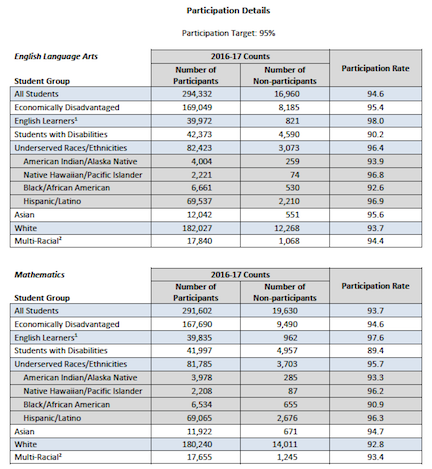
\includegraphics{Figures/Participation/Participation.png}

\subsection{Critical Element 2 - Assessment System
Operations}\label{critical-element-2---assessment-system-operations}

\subsubsection{2.1 Test Design and
Development}\label{test-design-and-development}

The test specifications document that describes our approach to
assessment and test design for the ORExt is published in \emph{Appendix}
2.1. The document includes our approach to reducing the depth, breadth,
and complexity (RDBC) of grade level content standards, an overview of
the essentialization process and EAF documents, the planned test design
for the ORExt, test development considerations, sample test items, item
specifications, and universal tools/designated supports/accommodations.
Only Grade 7 Math field test items were developed in 2017-18 which were
in accordance with the 2014-15 test specifications, and are the most
current available.

\paragraph{2.1A ORExt Purpose}\label{a-orext-purpose}

The stated purpose of the ORExt is to provide the state technically
adequate student performance data to ascertain proficiency on grade
level state content standards for students with significant cognitive
disabilities. A long-term goal of the program is to also provide
information regarding annual student growth related to these content
standards over Grades 3-8, as measured by vertically scaled assessments
in ELA and mathematics. The results of the assessment are currently
reported in comparison to four performance levels: Level 1, Level 2,
Level 3, and Level 4. Levels 3 and 4 denote a proficient level of
performance, while Levels 1 and 2 denote performance that is not
proficient. BRT and ODE developed a scaled score interpretation guide to
assist stakeholders in interpreting the meaning of the scaled scores
generated by the ORExt, supported by the state's achievement level
descriptors. This guidance is published in \emph{Appendix} 2.1A.

\paragraph{2.1B ORExt Test Blueprint}\label{b-orext-test-blueprint}

\emph{Appendix} 2.1B includes the entire test blueprint for the ORExt,
as conveyed by the balance of representation across content areas and
domains. Field-testing is conducted each year in order to support the
continuous improvement of test functioning. However, items are selected
to maintain this balance of representation. Oregon teachers validated
the content of the assessment, agreeing with the standards that were and
were not selected to develop the Essentialized Standards to which the
ORExt test items are aligned.

\paragraph{2.1C Test Development
Processes}\label{c-test-development-processes}

The test development process implemented for the ORExt is conveyed in
\emph{Appendix} 2.1C, including standard selection and validation, item
development, item review, review of all Oregon teacher feedback and
updating of items, and scaling and item selection. The \emph{Appendix}
articulates the process used to generate the materials with comma
separated value files used to create item templates that fed into Adobe
InDesign© through a data merge. Final test packages are reviewed for
accuracy and content and then disseminated via secure file transfer to
Oregon Qualified Assessors.

\paragraph{2.1D Computer-Adaptive
Considerations}\label{d-computer-adaptive-considerations}

The ORExt is not a computer-adaptive instrument, so these concerns do
not apply.

\subsubsection{2.2 Item Development}\label{item-development}

Item writers were recruited by ODE staff using an existing Qualified
Assessor/Qualified Trainer listserv. \FloatBarrier
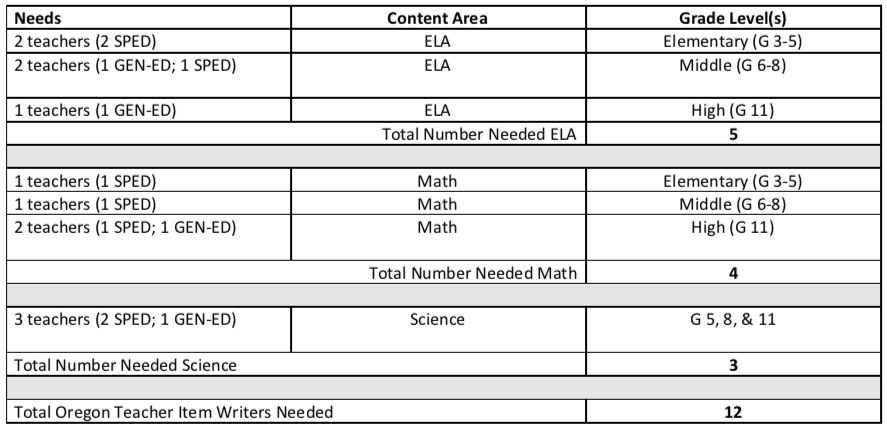
\includegraphics{Figures/ItemDev/ItemDev.png}

\paragraph{Project Description:}\label{project-description}

Behavioral Research and Teaching at the University of Oregon recruited
Oregon teachers to participate in item development for a new alternate
assessment. Selected teachers were asked to develop 360 items in English
Language Arts, Mathematics, or Science over the course of the summer,
from mid-June through end of August. The Project Director worked with
lead item developers to provide training, ongoing review and feedback,
and quality assurance. All participants were expected to provide
documentation of their qualifications and sign test security agreements.
In addition, all item developers were expected to participate in a
half-day item development training based upon the following schedule:
ELA - Tuesday, from 8 AM to 12 PM; Math - Wednesday, from 8 AM to 12 PM;
Science - Thursday, from 8 AM to 12 PM.

\paragraph{Minimum Qualifications:}\label{minimum-qualifications}

All licensed Oregon public school teachers with at least three years of
teaching in a life skills/severe needs program (SPED) or a general
education classroom (GEN-ED), respectively, were encouraged to apply.
Preference was given for item writing experience, additional years of
teaching experience, and higher education degree status.

\paragraph{Compensation:}\label{compensation}

Teachers who participated in this process were compensated at a rate of
\$20/hr via professional service contracts. It was anticipated that
teachers would produce 4 ELA items/hr, 6 Science items/hr, and 8 Math
items/hr. As such, the maximum contract amount for ELA was \$1,800, for
Science \$1,440, and for Math \$900. Item development focused primarily
on writing the stem and 3 options, with no need to produce graphics
(rather use labels for a BRT graphic designer to produce).

\paragraph{Contact:}\label{contact}

Because the timeline required work over the summer, Oregon teacher
recruitment was challenging. BRT researchers thus performed an
additional on-campus recruitment within the College of Education using
the same information. The final pool of item writers included 18 item
writers: seven Oregon teachers (all with MA degrees), five PhD
candidates within the COE, and six BRT researchers (four PhD candidates,
one PhD, and one with an MA). Item writers averaged 11.5 years of
teaching experience. The teachers recruited all had prior experience
developing items for the ORExt, as did all of the BRT researchers. The
five PhD candidates within the COE had no prior item development
experience. All item development was reviewed by BRT researchers and the
Project Manager.

The item development process followed is elaborated in \emph{Appendix}
2.2.1, which is the PowerPoint used in training all Oregon item writers.
The item development process was structured with the following steps.
Item writers were first oriented to the student population, as the pool
of item writers included both content and special education experts. The
Essentialization Process used to RDBC grade level standards was then
modeled so writers would understand how the item alignment targets, the
Essentialized Standards, were generated. Lecture, guided practice, and
independent practice activities and follow-up discussion ensured
comprehension of the process. BRT staff developed exemplar items for
every Essentialized Standard, varying the complexity from Low (L) to
Medium (M) to High (H) levels of complexity to convey the different
performance expectations at each level. The balanced vertical scaling
design provided an overall form-to-form and grade-to-grade level
framework for the test formation process once items were developed (see
\emph{Appendix} 2.2.2). Sample items are provided in \emph{Appendix}
2.2.3 for stakeholder reference, demonstrating the format and style of
typical items on the ORExt.

\subsubsection{2.3 Test Administration}\label{test-administration}

The ORExt assessments are administered according to the administration,
scoring, analysis, and reporting criteria established in the ORExt
General Administration Manual (see \emph{Appendix} 2.3). Important
updates to the testing process are distributed via the
\color{link}\href{http://www.oregon.gov/ode/educator-resources/assessment/Pages/Assessment-and-Accountability-Update.aspx}{Assessment
and Accountability Updates} \color{black} listserve, as well. ODE uses
this system to communicate information that is relevant for the
statewide assessment system, including the ORExt. Announcements are sent
to the listserv by email and are also posted to the ODE website. The
standardization of test administration is supported by a comprehensive
training process described below in Section 2.3B.

\paragraph{2.3A Administration and
Accommodations}\label{a-administration-and-accommodations}

The state has ensured that appropriate universal tools, designated
supports, and accommodations are available to students with disabilities
and students covered by Section 504 by providing guidance and technical
support on accommodations (see \emph{Appendices} 2.3A.1 and 2.3A.2).
Guidelines regarding use of the accommodations for instructional
purposes are included in the document, as all students are expected to
receive test accommodations that are consistent with instructional
accommodations.

Accommodations are built into the flexibility provided by the ORExt test
though they have not yet been researched for the ORExt. However, annual
training and proficiency testing efforts related to becoming a qualified
assessor and/or qualified trainer for the ORExt support standardized use
of available accommodations that are not already part of the test
design. Based on annual analyses, results demonstrate that student
performance varies according to their abilities and not
construct-irrelevant factors, such as sex, race, or ethnicity (See
Section 4.2).

The state has ensured that appropriate accommodations are available to
students with limited English proficiency by providing guidance and
technical support on accommodations (see \emph{Appendix} 2.3A.1).
Communication systems for this student population are limited; exposure
to multiple languages can make a student's communication system more
complex. The ORExt uses universal design principles and simplified
language approaches in order to increase language access to test content
for all students. In addition, directions and prompts may be
translated/interpreted for students in their native language.

An analysis of accommodated versus non-accommodated administrations is
needed in order to demonstrate that the provision of language
accommodations is not providing any advantage to students with limited
English proficiency, nor any disadvantage to other participants.
Accommodations information was collected this year as an option for data
entry. Entering accommodations information will be required next year.
Analyses of the impact of accommodation provision on the ORExt should
thus be feasible after the spring 2018 administration.

The Oregon Extended assessments can be administered using both Large
Print and Braille (contracted and non-contracted) versions, as well.
Oregon has ensured that the Oregon Extended assessments provide an
appropriate variety of accommodations for students with disabilities.
The state has provided guidance on accommodations in presentation,
response, setting, and timing in the Accommodations Manual 2013-14: How
to Select, Administer, and Evaluate Accommodations for Oregon's
Statewide Assessments (see \emph{Appendix} 2.3A.2). The Oregon Extended
assessments are also designed according to universal design principles
and utilize a simplified language approach (see \emph{Appendix} 2.3A.3).

In the 2013-2014 school year, the state developed a training and
proficiency program for sign language interpretation of its assessments
and has updated the site annually since that time. The
\color{link}\href{http://lms.brtprojects.org}{sign language training}
\color{black} process included videos of interpreters administering
items to students, materials that support appropriate administration
(i.e., transcripts and PowerPoint slides that supplement the video
administrations and the current ODE accommodations manual), and
proficiency testing to support standardized interpretation for Oregon's
assessments, including the ORExt. A 10-item proficiency test was
administered, with an 80\% required for passing (8/10 items correct). In
2017-18, the site was used to train 61 participants. All participants
passed the assessment on the first attempt. The overall average score on
the proficiency test was 95.9\%.

The ORExt assessments provide an appropriate variety of linguistic
accommodations for students with limited English proficiency. They also
use a simplified language approach in test development in order to
reduce language load of all items systematically (see \emph{Appendix}
2.3A3). Any given student's communication system may include home signs,
school signs, English words, and Spanish words, for example. With the
exception of items that require independent reading, the ORExt
assessment can be translated or interpreted by a Qualified Assessor (QA)
working with an interpreter in the student's native language, including
American Sign Language. QAs are allowed to translate/interpret the test
directions. QAs can adapt the assessment to meet the needs of the
student, while still maintaining standardization due to systematic
prompts and well-defined answers.

\paragraph{2.3B Comprehensive Training
System}\label{b-comprehensive-training-system}

Comprehensive information for ongoing training for all qualified
assessors (QAs) and Qualified Trainers (QTs) is provided in
\emph{Appendices} 2.3B.1-2.3B.8. Through an online distribution and
assessment system, \color{link}\href{https://or.k12test.com/}{QA/QT
Training and Proficiency} \color{black} is determined anually. This
website hosts all resources and information needed to administer, score,
report, and interpret the results from the ORExt. The website also
includes proficiency assessments that are required for all QAs and QTs
who may administer the ORExt. QTs are directly trained by ODE and BRT
staff as part of a train the trainers model. QTs then provide direct
trainings for new QAs in their respective regions.

The Oregon Department of Education (ODE) provided four direct statewide
trainings for new Qualified Trainers (QTs) and Qualified Assessors (QAs)
in face-to-face regional trainings. The schedule for the regional
trainings, as well as relevant training information, is provided below:
\FloatBarrier
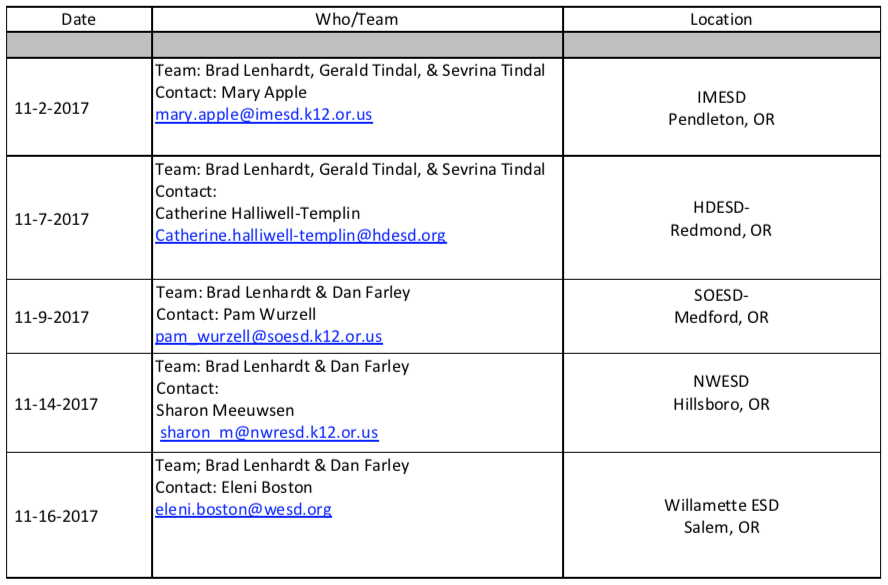
\includegraphics{Figures/TrainingSched/TraingSched.png}

Only trained Qualified Assessors (QAs) can administer the Oregon
Extended assessment. Qualified Assessors who also receive direct
instruction from ODE and BRT may become Qualified Trainers (QTs) who are
certified to train local staff using the train-the-trainers model.
Training for new assessors must be completed on an annual basis.
Assessors who do not maintain their respective certifications for any
given year must re-train if they choose to enter the system again.

The tables below contain data from the
\color{link}\href{http://or.k12test.com/}{Oregon Extended Assessment
Training and Proficiency Website} \color{black}. All assessors need to
complete some form of training each year to retain their status for
administering the Extended Assessments.

New assessors and returning assessors who needed further training in
2017-18 were required to pass four proficiencies with a score of 80\% or
higher. These four proficiencies were in Administration, English
Language Arts (ELA), Mathematics, and Science. Returning QAs or QTs for
the 2017-18 school year only needed to pass a Refresher Proficiency,
again with a score of 80\% or higher. The tables below contain data on
the number of assessors (participants) in each of the four
proficiencies, as well as the Refresher Proficiency. Included in the
data is the number of attempts needed to attain a passing score as well
as the average passing score of the participants.

An analysis of the Oregon Extended Assessment Training and Proficiency
Website showed 408 Assessors in-Training, 940 Qualified Assessors, and
139 Qualified Trainers. \FloatBarrier
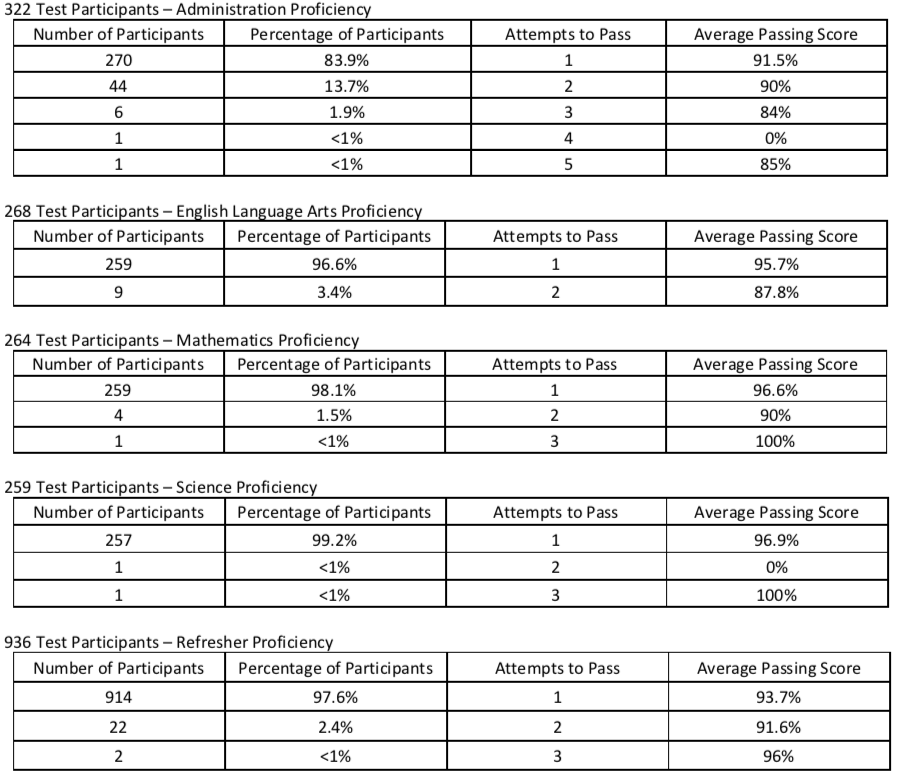
\includegraphics{Figures/TestPartic/TestParticipants.png}

A higher number of assessors completed the Refresher Proficiency test
than the subject area proficiency tests reflecting a greater number of
return assessors compared to new assessors. Administration Proficiency
continued to be the most challenging to new assessors, but most were
able to pass on the first or second attempt with about 1\% or less of
assessors requiring more than two attempts. The majority of assessors
passed the ELA, Math, Science, and the Refresher proficiency tests on
the first attempt with less than 2\% requiring a second or third
attempt. There were 7 fewer Qualified Assessors and 4 fewer Qualified
Trainers compared to last year.

Evaluations are collected at each QT training in November. The results
reflect general approval, but also suggest areas of improvement that ODE
and BRT work on for subsequent trainings/subsequent years, as
appropriate. QT evaluations this year included positively worded
statements regarding the quality of training rated on a scale where 1 =
Strongly Disagree, 2 = Disagree, 3 = Agree, and 4 = Strongly Agree.

The first section evaluated the state-level information and the
knowledge of the ODE presenters, the participants' level of comfort with
the training provided, the participants' ability to carry this training
and materials back to train district staff, and the overall utility of
the training. Seventy-six percent of participants strongly agreed with
these statements, 24\% agreed, and less than 3\% disagreed and strongly
disagreed, collectively. In the second section, participants were asked
to evaluate the BRT trainers and their guidelines regarding how to use
the training and proficiency website and related resources. Seventy-nine
percent of participants strongly agreed with these statements, 19\%
agreed, and less than 2\% disagreed and strongly disagreed,
collectively. Overall, these results demonstrate that participants felt
that the training was high quality and they felt confident that they
could train their staff upon return to their respective districts with
the knowledge and resources gained. This year's QT training cycle
included an optional afternoon session for any interested educators on
how to essentialize grade level content standards and how to develop
curriculum and provide instruction that is aligned to those standards
for students who are functioning off grade level, with a focus on
students with significant cognitive disabilities (SWSCD). We asked
participants to rate their confidence in using the knowledge acquired
during the session as well as to evaluate the quality of the
presentation and materials. A four-point scale was employed (Strongly
Disagree, Disagree, Agree, Strongly Agree). Percentages of responses for
each statement used in the survey are provided below. The table provides
a summary of the data related to participant confidence and their
evaluation of the quality of the presentation. The respondent n-sizes
ranged from 26-30, depending upon the question.

Note: Results are very positive, with some reviewers feeling less
confident about their abilities to train others about the
essentialization process. This outcome was expected. The process is
complex, particularly given the understanding that this was the first
time they had received such training. \FloatBarrier
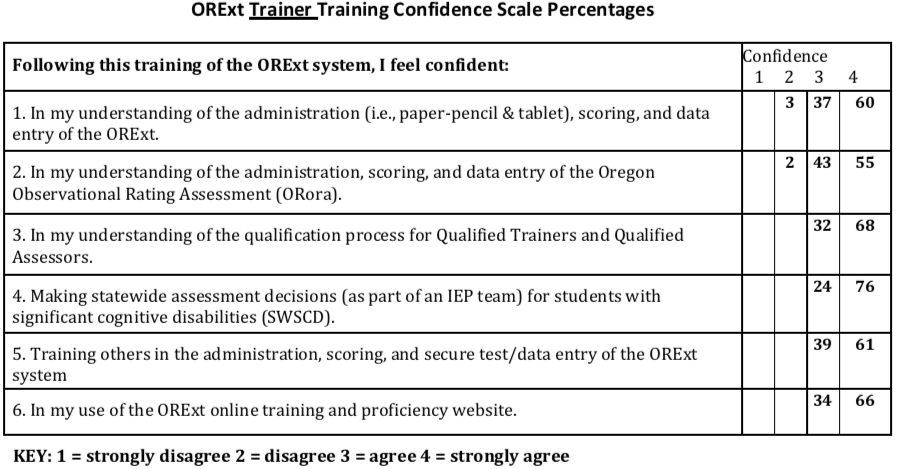
\includegraphics{Figures/QTQAtraining/TrainingConfidenceScale.png}

In addition, all technical assistance questions that we receive from the
field as part of our \emph{HelpDesk} are documented. The log of the
technical assistance provision is reviewed each month, as well as
annually, in order to determine what aspects of our assessment system
need further clarification or improvement. With the launch of the full
tablet app the helpdesk received many more inquiries than in previous
years. Around 48\% of the inquiries were end user issues such as slow
internet connection, trouble with individual tablets, users needing the
exit pin, etc. About 29\% of inquiries related to the ODE database. This
included things like credential verification, districts with no
Qualified Trainer, and students registered in different districts not
appearing on rosters. About 11\% of inquiries were coded as `Training'
indicating many of these issues could be solved with more emphasis on
certain areas during the fall trainings. Only 9\% of inquiries were
specific to the BRT tablet system and will be addressed in updates for
the 2018-19 testing window. And only 3\% of inquiries were related to
the paper/pencil administration.

The \emph{HelpDesk} log is published in \emph{Appendix} 2.3B.9.

Oregon monitors the quality of its system in several ways in order to
support continuous improvement. In terms of the assessment quality, item
statistics are reviewed each year and items that are not functioning as
intended are removed and replaced by better functioning field-test
items.

In 2014-15, items were reviewed in two phases, first using classical
test theory (CTT) and second using Rasch analyses. All items flagged as
a result of the statistical reviews were analyzed, item-by-item, by a
team of measurement and content experts at BRT. Not all flagged items
were removed, as several did not have apparent design flaws.
Considerations regarding domain representation as well as item
difficulty range also were considered during the review process. We also
employed different decision rules for unique items versus horizontally-
or vertically-scaled anchor items. It was important in many cases to
maintain anchor items. Items with clear design flaws were removed from
subsequent analyses and reporting. The following flagging criteria were
employed:

\clearpage
* \textbf{CTT}: A unique item was flagged if it had a p-value of .10 or
lower, .90 or higher, or a point biserial \textless{} .15. Anchor items
were flagged if they had a p-value of .10 or lower or .95 and higher on
all forms or a point biserial \textless{} .45 on any form. *
\textbf{Rasch}: Unique items were flagged if their outfit mean square
values were between 0 and .25 or \textgreater{} 1.5. Anchor items were
flagged if their outfit mean square values were \textless{} .5,
\textgreater{} 1.8 for horizontal items, or \textgreater{} 2.0 for
vertical anchor items.

Out of a total of 5,929 items developed in 2014-15, 166 were removed
(2.8\%).

We also implement a consequential validity study each year that surveys
QAs and QTs regarding the academic and social consequences of the ORExt,
both intended and unintended. The Consequential Validity report is
published in \emph{Appendix} 2.3B.10. ODE and BRT staff review the
results of the survey annually to determine what program improvements
are needed. A summary of the results is provided below.

ODE implemented a research survey program to address the need to
document the consequences, both intended and unintended, of the ORExt
Assessments. The research questions have been framed based upon current
consequential validity approaches for alternate assessments in the
literature, as well as issues that are of specific value in Oregon. The
survey included 121 respondents. This was 11\% of the solicited
respondents, who were all Qualified Assessors (QAs) and Qualified
Trainers (QTs) in the or.k12test.com database. The sample was 83\%
female and represented all regions of the state, as well as age ranges.
The survey included a range of quantitative and qualitative components.
The quantitative results demonstrate that QAs and QTs continue to feel
that the ORExt test items were easy to administer and score (64.2\%
Strongly Agree) and felt confident in their ability to interpret scaled
scores and Achievement Level Descriptors for the ORExt (69.8\% Strongly
Agree and Agree). They also felt that the items were accessible for
students who participated (78\% Strongly Agree and Agree) and that the
ORExt reflected the academic content that SWSCD should be learning
(68.4\% Strongly Agree and Agree). QAs and QTs felt marginally positive
about the educational impacts of the ORExt and marginally negative about
its social impacts. The results again demonstrate that the ORExt content
area assessments generally require up to one hour to administer.

The qualitative results revealed two areas in which educators
appreciated the ORExt and four areas of needed improvement. QAs and QTs
said that they appreciated: 1) the assessment's efficiency (i.e., more
streamlined administration, ease of administration, easier to give and
score online, online materials distribution); and, 2) overall item and
test design (i.e., one item per page, visual supports, scoring protocol
and student materials design, accessibility of test questions). Teachers
recommended the following areas of improvement, not all of which are
actionable: 1) Option to administer the assessment electronically, 2) A
functional skills assessment, 3) New items for very low functioning
students should be developed, and 4) A math assessment composed of more
practical/life skills problems involving time and money. Complete
results, including anticipated responses, from the survey can be found
in \emph{Appendix} 2.3B.10.

\paragraph{2.3C Technology-based
Assessments}\label{c-technology-based-assessments}

The ORExt was implemented using a technology-based platform as Phase 3
of the ORExt Tablet Administration. The 2017-18 testing window was the
first year all grade level and subject area assessments were available
on a tablet application/web-based platform. Administration of the tablet
application mirrors paper/pencil administration with each item read
aloud to the student, and the student asked to select one of three
answer choices. Tablet functionality includes optional discontinuation
if the student misses 10 out of the first 15 items, directing the
assessor to administer the ORora. To support understanding of the system
by both teachers and students, a separate practice test tablet
application is available. Helpdesk inquiries and feedback from the field
indicated much preference of the tablet administration versus
paper/pencil. Qualified Trainers and Qualified Assessors reported their
students' were more focused during tablet administration, and because
the tablet application scores automatically it was much more efficient
for assessors. Based on data and feedback from the field, improvements
will be made to the tablet application/web-based platform, and
additional training will be provided for the 2018-19 testing year. The
paper/pencil version will continue to be available for students who
cannot access a tablet administration. For the 2017-18 testing window,
data entry for the paper/pencil version was maintained by ODE. Beginning
in 2018-19, all test platforms and data entry will be through the BRT
servers, monitored by BRT.

\subsubsection{2.4 Monitoring Test
Administration}\label{monitoring-test-administration}

The ODE maintains a rigorous training system to support standardized
test administration for the \color{link}
\href{https://or.k12test.com}{Oregon K12 website}\color{black}, (secure
website, but see screenshot below for an example of training content).
\FloatBarrier
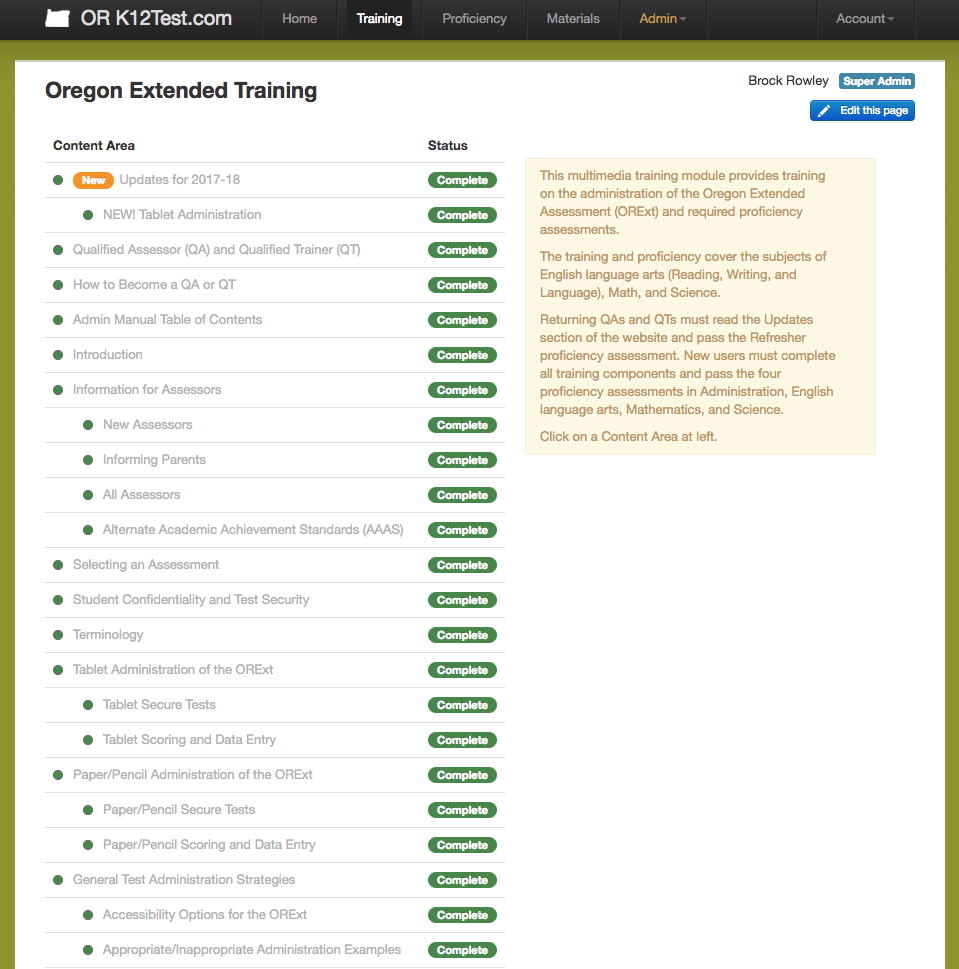
\includegraphics{Figures/TrainingSite/TrainingSite.png}

The or.k12test.com website includes a training section that addresses
any systems updates, the process for becoming a Qualified Assessor or
Qualified Trainer, student eligibility expectations, student
confidentiality and test security, test administration and scoring
expectations, examples of appropriate and inappropriate administration
(video), supporting student access to items without violating the test
construct, content area trainings that demonstrate how to administer
items in ELA, Math, and Science (video, with supporting test materials),
and how to access secure tests and complete data entry. Information for
QAs, QTs, and parents regarding the ORExt is also provided, as are all
necessary support materials. For QAs, these materials include practice
tests to prepare both themselves and students for the annual assessment
and all of the training materials used on the website. In addition to
these materials, QTs have access to all training materials necessary to
provide annual training to QAs in their purview (see screenshot below):
\FloatBarrier  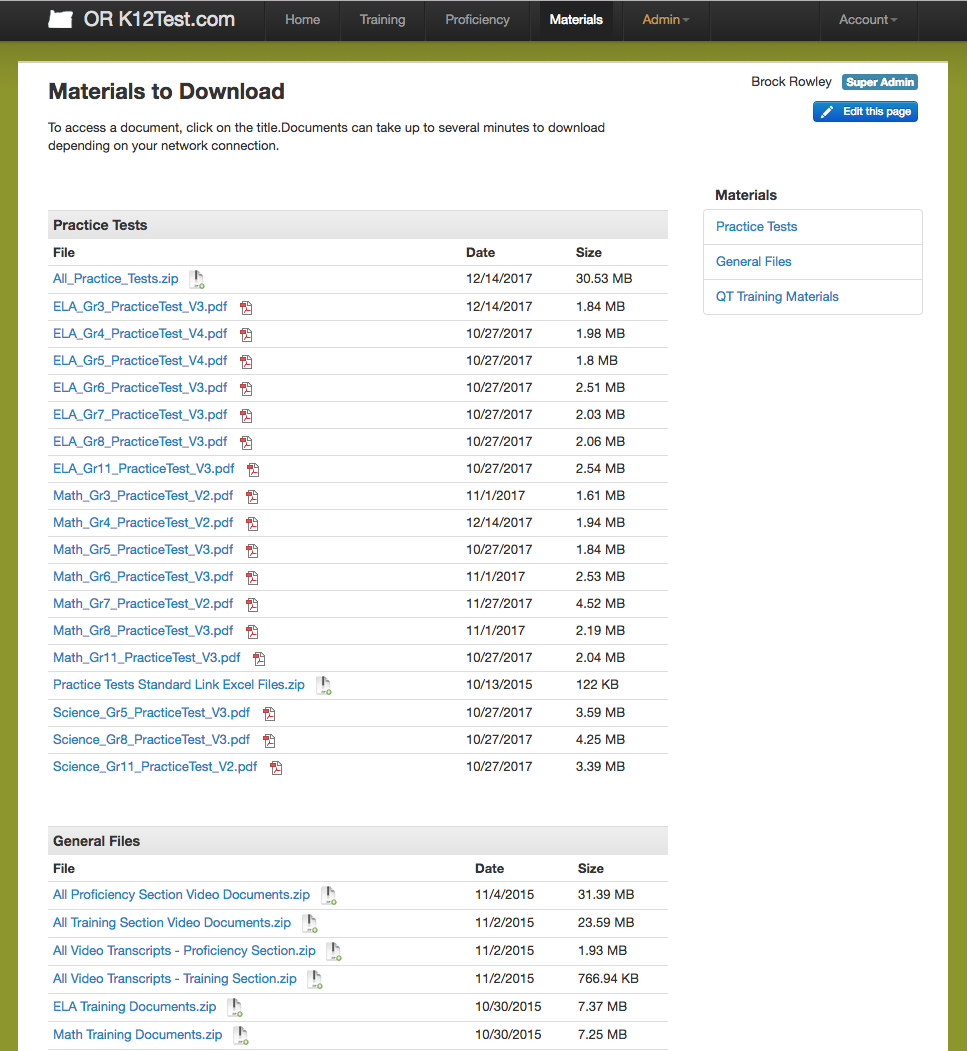
\includegraphics{Figures/TrainingSite/Downloads.png}

In addition, monitoring and reporting related to test administration
issues for the ORExt is addressed via general ODE reporting systems.
Information regarding this process can be located in the general
assessment system Peer Review evidence submission. \clearpage

\subsubsection{2.5 Test Security}\label{test-security}

\paragraph{2.5A Prevention of Assessment
Irregularities}\label{a-prevention-of-assessment-irregularities}

Test security policies and consequences for violation are addressed in
the Test Administration Manual on an annual basis (see \emph{Appendix}
1.4.2, p.~29-33). These policies include test material security, proper
test preparation guidelines and administration procedures, consequences
for confirmed violations of test security, and annual training
requirements at the district and school levels for all individuals
involved in test administration. Consequences for adult-initiated test
irregularities may be severe, including placing teaching licenses in
jeopardy (see \emph{Appendix} 1.4.2, p.~31-33).

\paragraph{2.5B Detection of Test
Irregularities}\label{b-detection-of-test-irregularities}

The ODE utilizes a localized monitoring system where school test
coordinators oversee building-level administration by trained, Qualified
Assessors, and report to centralized district test coordinators, who are
then responsible for reporting any confirmed violations to ODE.
Improprieties are defined as adult-initiated or student-initiated and
investigated accordingly (see \emph{Appendix} 1.4.2, p.~29-31).

\paragraph{2.5C Remediation Following Test Security
Incidents}\label{c-remediation-following-test-security-incidents}

ODE's alternate assessment program manager investigates and remediates
substantiated test security incidents for the ORExt by working with
district test coordinators. Additional information regarding this
process can be located in the general assessment system Peer Review
evidence submission.

\paragraph{2.5D Investigation of Test
Irregularities}\label{d-investigation-of-test-irregularities}

School and district test coordinators conduct initial investigations
into all alleged test irregularities. Once reported to ODE, all alleged
test irregularities are investigated in consultation with district test
coordinators and the test vendor, as appropriate (see \emph{Appendix}
1.4.2, p.~31-33). In the event that a test irregularity is determined to
be factual, consequences are determined based upon contextual issues
that are brought to light during the investigation. Additional
information regarding this process can be located in the general
assessment system Peer Review evidence submission.

\subsubsection{2.6 Systems for Protecting Data Integrity and
Privacy}\label{systems-for-protecting-data-integrity-and-privacy}

\paragraph{2.6A Integrity of Test
Materials}\label{a-integrity-of-test-materials}

Test materials for the ORExt are maintained throughout development,
dissemination, and administration via multiple mechanisms. All items
under development are stored in secure file servers managed by
Behavioral Research \& Teaching at the University of Oregon, the test
vendor for the ORExt. Item reviews necessary to provide alignment, bias,
and sensitivity information are conducted online using the secure
\color{link}\href{http://brtitemreview.com}{Distributed Item Review
(DIR)} \color{black} platform (secure website, but see \emph{Appendix}
3.1B for a system overview).

For the 2017-2018 school year, all paper/pencil secure test distribution
and data entry was hosted by
\color{link}\href{https://district.ode.state.or.us/apps/login/}{ODE's
secure file transfer system} \color
{black}, which is a password-protected test distribution and data entry
system. A data entry guide is provided in \emph{Appendix} 2.6.

The secure tablet application and web-based platform distribution and
data entry were hosted by BRT servers. All technology based secure
administration and data entry was password-protected. Download of the
tablet app was dependent on the type of device, all instructions and
download links were available in the Test App User Guide (see
\emph{Appendix} 2.6A)

\begin{figure}
\centering
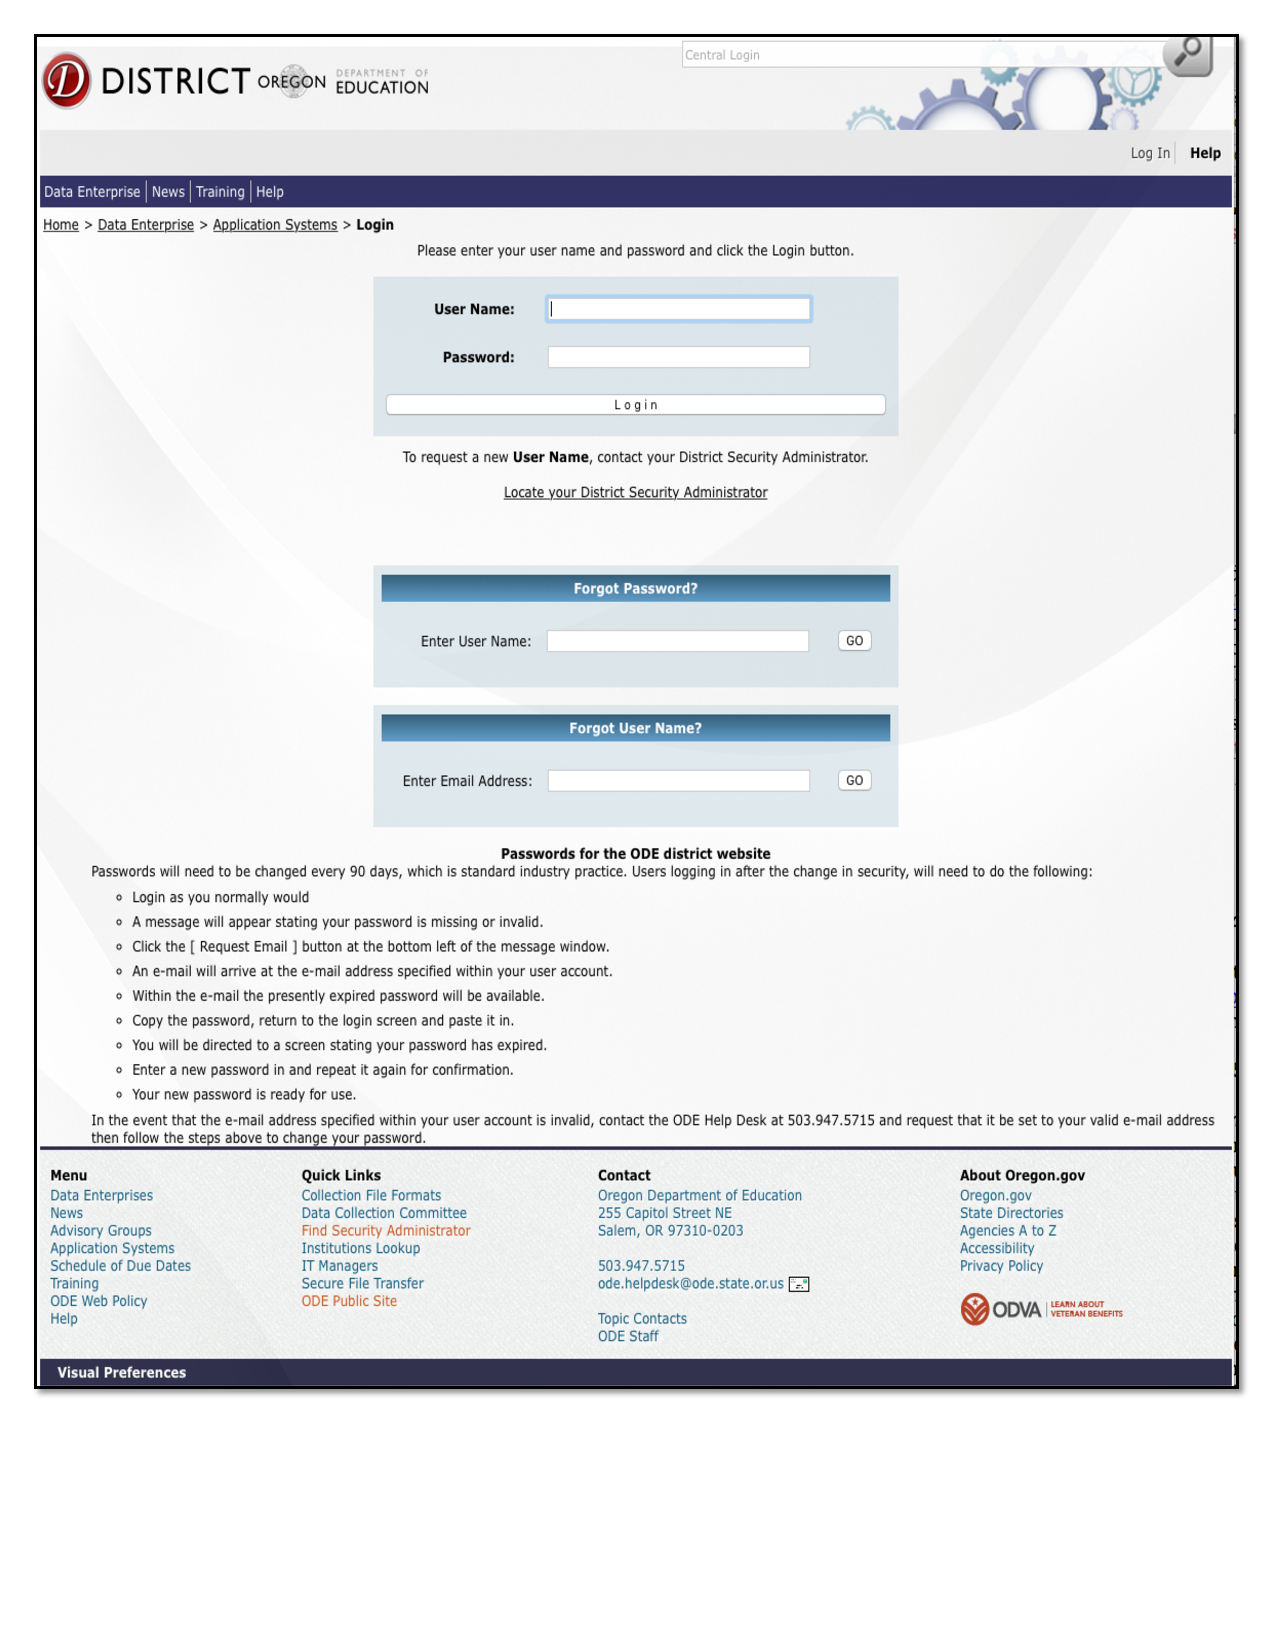
\includegraphics{Figures/TrainingSite/SecureSite.pdf}
\caption{}
\end{figure}

Additional information regarding test security can be located in the
general assessment system Peer Review evidence submission.

\paragraph{2.6B Secure Student-Level Assessment
Data}\label{b-secure-student-level-assessment-data}

Student level data is protected by relevant training and through a
secure data system in which all data entry is conducted online using
password-protected, secure procedures on the \color{link}
\href{https://or.k12test.com}{Oregon K12 website} \color{black} or
\color{link} \href{https://district.ode.state.or.us/apps/login/}{ODE's
secure file transfer system} \color{black} website, as identified above.
Only trained users with a vested educational interest who have signed
test security agreements are authorized to access to online data entry
systems. See \emph{Appendix} 2.6 for additional data entry expectations
for 2017-18.

\paragraph{2.6C Protecting Personally Identifiable
Information}\label{c-protecting-personally-identifiable-information}

All confidential, personally identifiable student information is
protected by policy and supported by training (see \emph{Appendix}
1.4.2, p.~26). The minimum number of students necessary to allow
reporting of students and student subgroups varies by rating (i.e.,
achievement, growth, graduation, and school size), by level (i.e.,
school/district/state), and by number of years of assessment data
available. For example, to receive an achievement rating, schools must
have at least 40 tests for the two most recent school years in reading
or mathematics. Alternatively, small schools receive an achievement
rating if they have at least 40 tests over the most recent four years.
If a school does not have at least 40 tests over a four-year period,
they will not receive an achievement score (see \emph{Appendix} 2.6C).
Similar rules are applied to student subgroups, including students with
disabilities, English learners, and students from diverse racial/ethnic
backgrounds (see \emph{Appendix} 2.6C, p.~7).

\subsection{Critical Element 3 - Technical Quality:
Validity}\label{critical-element-3---technical-quality-validity}

\subsubsection{3.1 Overall Validity, Including Validity Based on
Content}\label{overall-validity-including-validity-based-on-content}

As elaborated by Messick (1989) , the validity argument involves a claim
with evidence evaluated to make a judgment. Three essential components
of assessment systems are necessary: (a) constructs (what to measure),
(b) the assessment instruments and processes (approaches to
measurement), and (c) use of the test results (for specific
populations). Validation is a judgment call on the degree to which each
of these components is clearly defined and adequately implemented.

Validity is a unitary concept with multifaceted processes of reasoning
about a desired interpretation of test scores and subsequent uses of
these test scores. In this process, we want answers for two important
questions. Regardless of whether the students tested have disabilities,
the questions are identical: (1) How valid is our interpretation of a
student's test score? and (2) How valid is it to use these scores in an
accountability system? Validity evidence may be documented at both the
item and total test levels. We use the Standards (AERA et al., 2014) in
documenting evidence on content coverage, response processes, internal
structure, and relations to other variables. This document follows the
essential data requirements of the federal government as needed in the
peer review process. The critical elements highlighted in Section 4 in
that document (with examples of acceptable evidence) include (a)
academic content standards, (b) academic achievement standards, (c) a
statewide assessment system, (d) reliability, (e) validity, and (f)
other dimensions of technical quality.

In this technical report, data are presented to support the claim that
Oregon's AA-AAAS provides the state technically adequate student
performance data to ascertain proficiency on grade level state content
standards for students with significant cognitive disabilities - which
is its defined purpose. The AA-AAAS are linked to grade level academic
content, generate reliable outcomes at the test level, include all
students, have a cogent internal structure, and fit within a network of
relations within and across various dimensions of content related to and
relevant for making proficiency decisions. Sample items that convey the
design and sample content of ORExt items are provided in \emph{Appendix}
2.2.3.

The assessments are administered and scored in a standardized manner.
Assessors who administer the ORExt are trained to provide the necessary
level of support for appropriate test administration on an item-by-item
basis. There are four levels of support outlined in training: full
physical support, partial physical support, prompted support, and no
support. Items were designed to document students' skill and knowledge
on grade level academic content standards, with the level of support
provided designed not to interfere with the construct being measured.
Only one test administration type is used for the ORExt, patterned after
the former Scaffold version of the assessment. Assessors administer the
prompt and if the student does not respond, the Assessor reads a
directive statement designed to focus the student's attention upon the
test item and then repeats the prompt. If the student still does not
respond, the Assessor repeats the prompt as needed and otherwise scores
the item as incorrect and moves on to the next item. Training
documentation is provided in \emph{Appendices} 2.3B.1-2.3B.8.

Given the content-related evidence that we present related to test
development, alignment, training, administration, scoring, the
reliability information reflected by adequate coefficients for tests,
and, finally, the relation of tests across subject areas (providing
criterion-related evidence), we conclude that the alternate assessment
judged against alternate achievement standards allows valid inferences
to be made on state accountability proficiency standards.

\paragraph{3.1A Alignment Between AA-AAAS and Academic Content
Standards}\label{a-alignment-between-aa-aaas-and-academic-content-standards}

Our foundation of validity evidence from content coverage for the ORExt
comes in the form of test specifications (see \emph{Appendix} 2.1) and
test blueprints (see \emph{Appendix} 2.1B). Among other things, the
Standards (AERA et al., 2014) suggest specifications should ``define the
content of the test, the proposed test length, the item
formats\ldots{}'' (Standard 4.2, p.~85).

All items are linked to grade level standards and a prototype was
developed using principles of universal design with traditional,
content-referenced multiple-choice item writing techniques. The most
important component in these initial steps addressed language complexity
and access to students using both receptive, as well as expressive,
communication. Additionally, both content breadth and depth were
addressed. We developed one test form for the ORExt that utilizes a
scaffold approach. This approach allows for students with very limited
attention to access test content, while the supports are not utilized
for students who do not need this support.

We developed the test iteratively by developing items (see
\emph{Appendix} 2.2.1, which conveys our item writer training
materials), piloting them, reviewing them, and editing successive
drafts. We used a combination of existing panels of veteran teachers who
have worked with the Oregon Department of Education (ODE) in various
advising roles on testing content in general and special education,
using the same processes and criteria, as well as the introduction of
newer teachers who are qualified as we proceed to remain relevant.
Behavioral Research and Teaching (BRT) personnel conducted the internal
reviews of content. After the internal development of prototype items,
all reviews then involved Oregon content and special education experts
with significant training and K-12 classroom experience.

The ORExt incorporates continuous improvement into its test design via
field-testing in all content areas on an annual basis, with an average
of 25\% new items. These items are compared to operational items based
on item functioning and test design factors, generating data used to
replace items on an annual basis, incorporating the new items that fill
a needed gap with regard to categorical concurrence, or provide for a
wider range of functioning with regard to complexity levels: low -
medium - high, comparable to Webb's DOK (see Section 2.2).

BRT employed a multi-stage development process in 2014-15 to ensure that
test items were linked to relevant content standards, were accessible
for students with significant cognitive disabilities, and that any
perceived item biases were eliminated. The item review process included
51 reviewers with an average of 22 years of experience in education. The
ORExt assessments have been determined to demonstrate strong linkage to
grade level academic content, overall. Full documentation of the initial
2014 linkage study and a new, independent alignment study conducted in
spring, 2017 is provided in \emph{Appendix} 3.1A. Based on student
performance from the 2016-2017 testing year, new and Grade 7 Math field
test items were written in fall 2017.

The summary section of the independent alignment study report states
that, ``Oregon's Extended Assessments (ORExt) in English Language Arts,
Mathematics, and Science were evaluated in a low-complexity alignment
study conducted in Spring of 2017. Averages of reviewer professional
judgments over five separate evaluations were gathered, reviewed, and
interpreted in the pages that follow. In the three evaluations that
involved determining the relationship between standards and items,
reviewers identified sufficient to strong relationships among assessment
components in all grades and all subject areas. In the two evaluations
involving Achievement Level Descriptors, reviewers identified thirty
instances of sufficient to strong relationships out of thirty-four
possible relationship opportunities resulting in an overall affirmed
relationship with areas for refinements identified.''

Because the assessments demonstrate sufficient to strong linkage to
Oregon's general education content standards and descriptive statistics
demonstrate that each content area assessment is functioning as
intended, it is appropriate to deduce that these standards define the
expectations that are being measured by the Oregon Extended assessments.

The Oregon Extended assessments yield scores that reflect the full range
of achievement implied by Oregon's alternate achievement standards.
Evidence of this claim is found in the standard setting documentation
submitted in Section 6.2. Standards were set for all subject areas on
June 15-17, 2015. Standards included achievement level descriptors and
cut scores, which define Oregon's new alternate achievement standards
(AAS). The State Board of Education officially adopted the AAS on June
25, 2015.

\paragraph{3.1B AA-AAAS Linkage to General Content
Standards}\label{b-aa-aaas-linkage-to-general-content-standards}

Results of the analysis of the linkage of the new Essentialized
Assessment Frameworks, (EAF), composed of Essentialized Standards
(EsSt), to grade level CCSS in English language arts and mathematics and
linked to ORSci and NGSS in science, are presented in Section 3.1A. The
claim is that the EsSt are sufficiently linked to grade level standards,
while the ORExt items are aligned to the EsSt. In addition to presenting
linkage information between grade level content standards and the EsSt,
the linkage study presents alignment information related to the items on
the new ORExt in comparison to the EsSt. Extended assessments have been
determined to link sufficiently to grade level academic content
standards. Field test items are added each year based on item alignment
to standards.

The Oregon Extended assessments link to grade level academic content, as
reflected in the item development process. Oregon also had each
operational item used on the Oregon Extended assessment evaluated for
alignment as part of two comprehensive linkage studies, one performed in
2014 and an independent alignment study performed in 2017 (see Section
3.1A). The professional reviewers in an internal study in 2014 and an
independent study in spring 2017 included both special and general
education experts, with content knowledge and experience in addition to
special education expertise.

According to the independent linkage study report, the spring 2017
review was conducted by expert reviewers with professional backgrounds
in either Special Education (the population), Assessment, or in Oregon's
adopted content standards. Reviewers were assigned to review grade-level
items relative to their experience and expertise. In all, 39 reviewers
participated. Thirty-four (34) participated in all 5 evaluations:
thirteen (13), for the English Language Arts review, fifteen (15) for
the Mathematics review, and six (6) for the Science review. All
participants were assigned to at least one specific content area as
shown in Table 1. Note: Four individuals were assigned to two areas of
review. The thirty-nine individuals who participated in the study had a
robust legacy of experience in the field and in the state. Participants
represented 25 unique school districts across the state representing
both urban and rural perspectives. All 39 of the individuals
participating in the study held current teaching licenses. Two
individuals also held administrative licenses. Years of experience in
their area ranged from 3 - 30 years of experience with an average of 17
years of experience. (Mode = 11 years, Median = 16 years). One
individual indicated 50 years of experience in the field. Three of the
39 individuals held a Bachelor's degree only. Thirty-six held a
Bachelor's degree and at least one Master's degree. Two held a
Bachelor's degree, at least one Master's degree, and a doctoral degree.
Fourteen (36\%) of the individuals identified as experts in a specific
Content area and 25 (64\%) of the individuals identified Special
education as their primary area of expertise.

These skilled reviewers were trained by synchronous webinars on
linkage/alignment, as well as item depth, breadth, and complexity and
then completed their ratings online via BRT's Distributed Item Review
(DIR) website and on Excel spreadsheets shared with the researcher
electronically (see \emph{Appendix} 3.1B for an overview). Mock linkage
ratings were conducted in order to address questions and ensure
appropriate calibration. Reviewers rated each essentialized standard on
a 3-point scale (0 = no link, 1= sufficient link, 2= strong link) as it
related to the standard the test developers had defined for that
essentialized standard. Items were evaluated, in turn, based upon their
alignment to the essentialized standard on a 3-point scale (0 =
insufficient alignment, 1 = sufficient alignment, 2 = strong alignment).
When averaged across reviewers, 1.00-1.29 was considered in the low
range, 1.30 - 1.69 was sufficient, and 1.70 - 2.0 was strong. Additional
comment was requested for any essentialized standard or item whose
linkage was rated 0.

Overall, the 2017 independent alignment study concludes that: ``First,
reviewers were asked to conduct an affirmational review of the rationale
used by test developers to omit certain content standards. This finding
was used to infer that the final standards selected for inclusion or
omission in Oregon's Extended Assessment were chosen rationally and that
the final scope of content standards can be considered justifiable for
the population for the subject area. Conclusion: This review, with a
lowest average rate of .82 (on a scale of 1), permits the inference: the
scope of the standards selected for translation to Essentialized
Standards were rationally selected. None of the standards de-selected
(for inaccessibility or for being covered elsewhere) were strongly
identified for re- inclusion, nor were identified as a critical hole for
this population of students. Second, reviewers were asked to identify
the strength of the link between the source standard and the
Essentialized Standard. This finding was used to infer that the process
undertaken to essentialize a given Source Standard did not fundamentally
or critically alter the knowledge or skill set intended by the source
standard for this population of students (further confirming that the
content selected for assessment is comparable). Conclusion:This review,
with a range of 1.5 - 1.9 (on a scale of 2) permits the inference: the
Essentialized Standards were found to link sufficiently to the source
standards on average beyond the''sufficient" average of 1.0. Third,
reviewers were asked to identify the strength of the alignment between
the Essentialized Standards and the items and to review the items
developed using the Essentialized Standards for bias, and accessibility.
The finding from this review was used to infer that the items written
for this grade and subject area (using these Essentialized Standards)
were adequately linked to the Essentialized Standards, were free from
bias, and were accessible to students with significant cognitive
disabilities. Conclusion: The alignment review (1.32 - 1.89),
accessibility review (.67 - 1.0), and freedom from bias review (.65 -
1.0) all permit the inference that the test items indicate a
relationship with the source standards, the test items are not overly
biased towards or against any particular group of individuals, and the
test items are written such that the content and intent can be accessed
by students with the most significant cognitive disabilities. (**Note:
this range was skewed by feedback from one reviewer --ELA-Grade 3 -
whose comments were noted in this study. Removing that individual's
comments would result in a range of .90 - 1.0 accessibility range and
.89 - 1.0 freedom from bias range respectively.) Fourth, reviewers were
asked to review the statements used to describe student achievement on
the test (the Achievement Level Descriptors) and their alignment to the
Essentialized Standards that the students were tested on. The finding
from this review was used to infer that the skills and achievements
described by the Achievement Level Descriptors for each subject and
grade level are aligned with the content standard being measured.
Conclusion: The reviews ranging from .68* - 1.0 permit the inference
that the descriptions made regarding student skillset are an accurate
reflection of the standards from which the assessment was developed at
all three levels evaluated. (*One outlier for ELA-Grade 4 provided a
review of a .52 average). Fifth, and finally, reviewers were asked to
review the alignment of the Achievement Level Descriptors to the items.
The finding from this review was used to infer that each item in the
developed assessment(s) was appropriately aligned to its associated
Achievement Level Descriptor (further confirming that decisions made
using this test were aligned with the intent of the source standard).
Conclusion: Fourteen of the seventeen grade-level reviews resulted in an
average reviewer range of .67 - 1.0 indicating an appropriate alignment
between ALDs and the items as written. This review permits the inference
that, overall, the Achievement Level Descriptors are accurate
reflections of the items. In three instances (Mathematics-Grades 3 and
4, and ELA-Grade 8) the average alignment by reviewer was .5 (indicating
that one of the two individuals in that category did not agree that the
items and ALDs were aligned)."

\subsubsection{3.2 Validity Based on Cognitive
Processes}\label{validity-based-on-cognitive-processes}

Evidence of content coverage is concerned with judgments about ``the
extent to which the content domain of a test represents the domain
defined in the test specifications'' (AERA et al., 2014, Standard 4.12,
p.~89)\textsuperscript{7}. As a whole, the ORExt is comprised of sets of
items that sample student performance on the intended domains. The
expectation is that the items cover the full range of intended domains,
with a sufficient number of items so that scores credibly represent
student knowledge and skills in those areas. Without a sufficient number
of items, the potential exists for a validity threat due to construct
under-representation (Messick, 1989)\textsuperscript{6}.

The ORExt assessment is built upon a variety of items that address a
wide range of performance expectations rooted in the CCSS, NGSS, and
ORSci content standards. The challenge built into the test design is
based first upon the content within each standard in English language
arts, mathematics, and science. That content is RDBC in a manner that is
verified by Oregon general and special education teachers to develop
assessment targets that are appropriate for students with the most
significant cognitive disabilities. Our assessments utilize universal
design principles in order to include all students in the assessment
process, while effectively challenging the higher performing students.
For students who have very limited to no communication and are unable to
access even the most accessible items on the ORExt, an Oregon
Observational Rating Assessment (ORora) was first implemented in
2015-16. The ORora is completed by teachers and documents the student's
level of communication complexity (expressive and receptive), as well as
level of independence in the domains of attention/joint attention and
mathematics. A complete report of ORora results from 2017-18 is provided
in \emph{Appendix} 5.1D.

Fifty-one reviewers analyzed all ORExt items for bias, sensitivity,
accessibility to the student population, and alignment to the
Essentialized Standards. A total of 21 reviewers were involved in the
English language arts item reviews. An additional 21 reviewers were
involved in the Mathematics item reviews. Science employed nine
reviewers. Reviewers were organized into grade level teams of two
special educators and one content specialist.

Substantive evidence that has been documented suggests that the ORExt
items are tapping the intended cognitive processes and that the items
are at the appropriate grade level through the linkage/alignment studies
documented above, including reviews of linkage, content coverage, and
depth of knowledge.

\subsubsection{3.3 Validity Based on Internal Structure (Content and
Function)}\label{validity-based-on-internal-structure-content-and-function}

The Oregon Extended assessments reflect patterns of emphasis that are
supported by Oregon educators as indicated by the following three tables
that highlight the balance of standard representation by grade level for
English language arts, mathematics, and science on the ORExt. The
representation ratios can be calculated by dividing the standards by the
total within each respective column. For example, in Grade 3 Reading,
approximately 25\% of the items are in the Reading Standards for
Literature domain, as that domain has 4 written Essentialized Standards
(EsSt) out of the total of 16 (4/16 = 25\%).

The test blue prints below directly correspond to the number of ES
written in each domain within the Essentialized Assessment Frameworks
(EAF) spreadsheets. There are additional grade level standards addressed
by the EsSt, as some EsSt link to multiple grade level content
standards. However, the blueprints below reflect only the written EsSt
and are thus an underrepresentation of the breadth of grade level
content addressed by the ORExt. \FloatBarrier
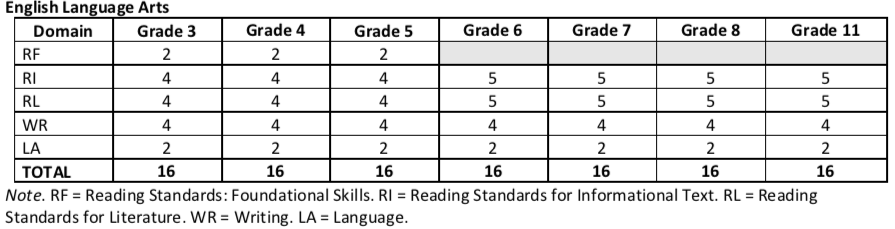
\includegraphics{Figures/EsSt/EsStELA.png} \clearpage

\FloatBarrier
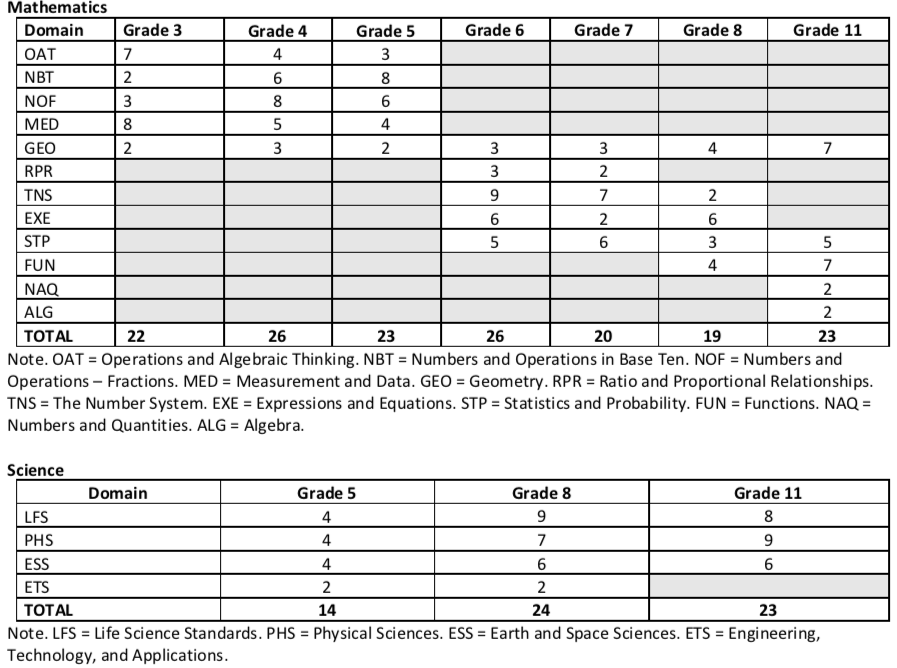
\includegraphics{Figures/EsSt/EsStMathScience.png} The primary purpose
of the ORExt assessment is to yield technically adequate performance
data on grade level state content standards for students with
significant cognitive disabilities in English language arts,
mathematics, and science at the test level. All scoring and reporting
structures mirror this design and have been shown to be reliable
measures at the test level (see Section 4.1). The process of addressing
any gaps or weaknesses in the system is accomplished via field-testing
(see Section 3.1A).

\paragraph{Point Measure Correlations}\label{point-measure-correlations}

Distributions of point measure correlations and outfit mean square
statistics for operational items are provided below, by content area and
grade. Point measure correlations display how the item scores correlate
with the latent overall score, while outfit mean square statistics
closer to 1.0 denote minimal distortion of the measurement system. All
items included in the 2017-18 operational assessment are represented.
Point measure correlations ranged from 0.34 to 0.74 in ELA, 0.12 to 0.71
in Math, to 0.25 to 0.74 in Science. All data visualizations were
conducted with ggplot in the tidyverse package (Wickham, H., 2017).

\clearpage
\FloatBarrier

\begin{table}[!h]

\caption{\label{tab:ifiles}Point Measure Correlations: English/Language Arts}
\centering
\begin{tabu} to \linewidth {>{\raggedleft}X>{\raggedleft}X>{\raggedleft}X>{\raggedleft}X}
\toprule
Grade & Mean & Min & Max\\
\midrule
3 & 0.55 & 0.36 & 0.66\\
4 & 0.59 & 0.39 & 0.69\\
5 & 0.63 & 0.49 & 0.70\\
6 & 0.62 & 0.49 & 0.72\\
7 & 0.62 & 0.34 & 0.70\\
\addlinespace
8 & 0.60 & 0.34 & 0.71\\
11 & 0.68 & 0.53 & 0.74\\
\bottomrule
\end{tabu}
\end{table}\begin{table}[!h]

\caption{\label{tab:ifiles}Point Measure Correlations: Math}
\centering
\begin{tabu} to \linewidth {>{\raggedleft}X>{\raggedleft}X>{\raggedleft}X>{\raggedleft}X}
\toprule
Grade & Mean & Min & Max\\
\midrule
3 & 0.48 & 0.12 & 0.70\\
4 & 0.46 & 0.20 & 0.63\\
5 & 0.42 & 0.22 & 0.69\\
6 & 0.45 & 0.21 & 0.71\\
7 & 0.44 & 0.16 & 0.71\\
\addlinespace
8 & 0.43 & 0.27 & 0.62\\
11 & 0.50 & 0.32 & 0.65\\
\bottomrule
\end{tabu}
\end{table}\begin{table}[!h]

\caption{\label{tab:ifiles}Point Measure Correlations: Science}
\centering
\begin{tabu} to \linewidth {>{\raggedleft}X>{\raggedleft}X>{\raggedleft}X>{\raggedleft}X}
\toprule
Grade & Mean & Min & Max\\
\midrule
5 & 0.58 & 0.25 & 0.71\\
8 & 0.62 & 0.46 & 0.71\\
11 & 0.65 & 0.31 & 0.74\\
\bottomrule
\end{tabu}
\end{table}

\paragraph{Outfit Mean Square
Distributions}\label{outfit-mean-square-distributions}

Outfit mean square values below 1.0 demonstrate that values are too
predictable and perhaps redundant, while values above 1.0 indicate
unpredictability. Items above 2.0 are deemed insufficient for
measurement purposes and flagged for replacement. While most OMS values
in ELA were between 0.5 and 1.5, one item in each Grade 6, 7, and 11 was
above 2.0 and will be removed. One item in Grade 7 Math and one item in
Grade 11 Science will also be removed.

\begin{table}[!h]

\caption{\label{tab:outfit}Mean Square Outfit: English/Language Arts}
\centering
\begin{tabu} to \linewidth {>{\raggedleft}X>{\raggedleft}X>{\raggedleft}X>{\raggedleft}X}
\toprule
Grade & Mean & Min & Max\\
\midrule
3 & 0.97 & 0.46 & 1.54\\
4 & 0.95 & 0.53 & 1.65\\
5 & 0.94 & 0.65 & 1.48\\
6 & 0.96 & 0.49 & 2.67\\
7 & 1.00 & 0.60 & 2.26\\
\addlinespace
8 & 0.93 & 0.50 & 1.98\\
11 & 0.90 & 0.40 & 2.22\\
\bottomrule
\end{tabu}
\end{table}\begin{table}[!h]

\caption{\label{tab:outfit}Mean Square Outfit: Math}
\centering
\begin{tabu} to \linewidth {>{\raggedleft}X>{\raggedleft}X>{\raggedleft}X>{\raggedleft}X}
\toprule
Grade & Mean & Min & Max\\
\midrule
3 & 1.00 & 0.66 & 1.82\\
4 & 1.01 & 0.69 & 1.58\\
5 & 1.03 & 0.79 & 1.40\\
6 & 0.95 & 0.68 & 1.37\\
7 & 0.98 & 0.60 & 2.47\\
\addlinespace
8 & 1.00 & 0.74 & 1.69\\
11 & 0.95 & 0.64 & 1.31\\
\bottomrule
\end{tabu}
\end{table}\begin{table}[!h]

\caption{\label{tab:outfit}Mean Square Outfit: Science}
\centering
\begin{tabu} to \linewidth {>{\raggedleft}X>{\raggedleft}X>{\raggedleft}X>{\raggedleft}X}
\toprule
Grade & Mean & Min & Max\\
\midrule
5 & 0.96 & 0.45 & 1.69\\
8 & 0.90 & 0.51 & 1.82\\
11 & 0.93 & 0.42 & 2.22\\
\bottomrule
\end{tabu}
\end{table}

\paragraph{Annual Measureable Objectives Frequencies \&
Percentages}\label{annual-measureable-objectives-frequencies-percentages}

Annual Measurable Objective (AMO) calculations were conducted based upon
student performance on the ORExt tied to the vertical scale using Rasch
modeling. Overall results are largely consistent with 2016-17, with
approximately 50\% of students with significant cognitive disabilities
achieving proficiency across grades and content areas. The data
visualizations presented below were conducted with ggplot in the
tidyverse package (Wickham, H., 2017).

\begin{table}[!h]

\caption{\label{tab:ode_data}English/Language Arts Percent Proficient By Grade}
\centering
\begin{tabu} to \linewidth {>{\raggedright}X>{\raggedleft}X>{\raggedleft}X>{\raggedleft}X>{\raggedleft}X}
\toprule
Grade & AMO Level 1 & AMO Level 2 & AMO Level 3 & AMO Level 4\\
\midrule
Grade 3 & 17 & 47 & 24 & 12\\
Grade 4 & 22 & 25 & 32 & 21\\
Grade 5 & 26 & 34 & 16 & 25\\
Grade 6 & 27 & 29 & 26 & 18\\
Grade 7 & 32 & 23 & 24 & 21\\
\addlinespace
Grade 8 & 36 & 24 & 23 & 17\\
Grade 11 & 19 & 25 & 11 & 45\\
Grade 12 & 4 & 12 & 4 & 79\\
\bottomrule
\end{tabu}
\end{table}\begin{table}[!h]

\caption{\label{tab:ode_data}Math Percent Proficient By Grade}
\centering
\begin{tabu} to \linewidth {>{\raggedright}X>{\raggedleft}X>{\raggedleft}X>{\raggedleft}X>{\raggedleft}X}
\toprule
Grade & AMO Level 1 & AMO Level 2 & AMO Level 3 & AMO Level 4\\
\midrule
Grade 3 & 38 & 24 & 33 & 4\\
Grade 4 & 25 & 41 & 29 & 5\\
Grade 5 & 19 & 46 & 31 & 5\\
Grade 6 & 49 & 18 & 32 & 2\\
Grade 7 & 53 & 12 & 33 & 2\\
\addlinespace
Grade 8 & 48 & 16 & 31 & 4\\
Grade 11 & 35 & 24 & 32 & 9\\
Grade 12 & 18 & 25 & 43 & 14\\
\bottomrule
\end{tabu}
\end{table}\begin{table}[!h]

\caption{\label{tab:ode_data}Reading Percent Proficient By Grade}
\centering
\begin{tabu} to \linewidth {>{\raggedright}X>{\raggedleft}X>{\raggedleft}X>{\raggedleft}X>{\raggedleft}X}
\toprule
Grade & AMO Level 1 & AMO Level 2 & AMO Level 3 & AMO Level 4\\
\midrule
Grade 3 & 19 & 42 & 30 & 9\\
Grade 4 & 21 & 26 & 33 & 20\\
Grade 5 & 24 & 31 & 19 & 26\\
Grade 6 & 29 & 27 & 26 & 18\\
Grade 7 & 32 & 23 & 30 & 15\\
\addlinespace
Grade 8 & 39 & 23 & 22 & 16\\
Grade 11 & 18 & 28 & 8 & 46\\
Grade 12 & 8 & 8 &  & 83\\
\bottomrule
\end{tabu}
\end{table}\begin{table}[!h]

\caption{\label{tab:ode_data}Science Percent Proficient By Grade}
\centering
\begin{tabu} to \linewidth {>{\raggedright}X>{\raggedleft}X>{\raggedleft}X>{\raggedleft}X>{\raggedleft}X}
\toprule
Grade & AMO Level 1 & AMO Level 2 & AMO Level 3 & AMO Level 4\\
\midrule
Grade 5 & 27 & 22 & 33 & 18\\
Grade 8 & 34 & 15 & 26 & 25\\
Grade 11 & 21 & 14 & 30 & 34\\
\bottomrule
\end{tabu}
\end{table}\begin{table}[!h]

\caption{\label{tab:ode_data}Writing Percent Proficient By Grade}
\centering
\begin{tabu} to \linewidth {>{\raggedright}X>{\raggedleft}X>{\raggedleft}X>{\raggedleft}X>{\raggedleft}X}
\toprule
Grade & AMO Level 1 & AMO Level 2 & AMO Level 3 & AMO Level 4\\
\midrule
Grade 3 & 27 & 41 & 15 & 17\\
Grade 4 & 25 & 20 & 21 & 34\\
Grade 5 & 29 & 33 & 10 & 28\\
Grade 6 & 30 & 30 & 11 & 29\\
Grade 7 & 37 & 20 & 28 & 14\\
\addlinespace
Grade 8 & 35 & 27 & 11 & 27\\
Grade 11 & 19 & 20 & 9 & 51\\
Grade 12 & 4 & 12 &  & 83\\
\bottomrule
\end{tabu}
\end{table}

\clearpage

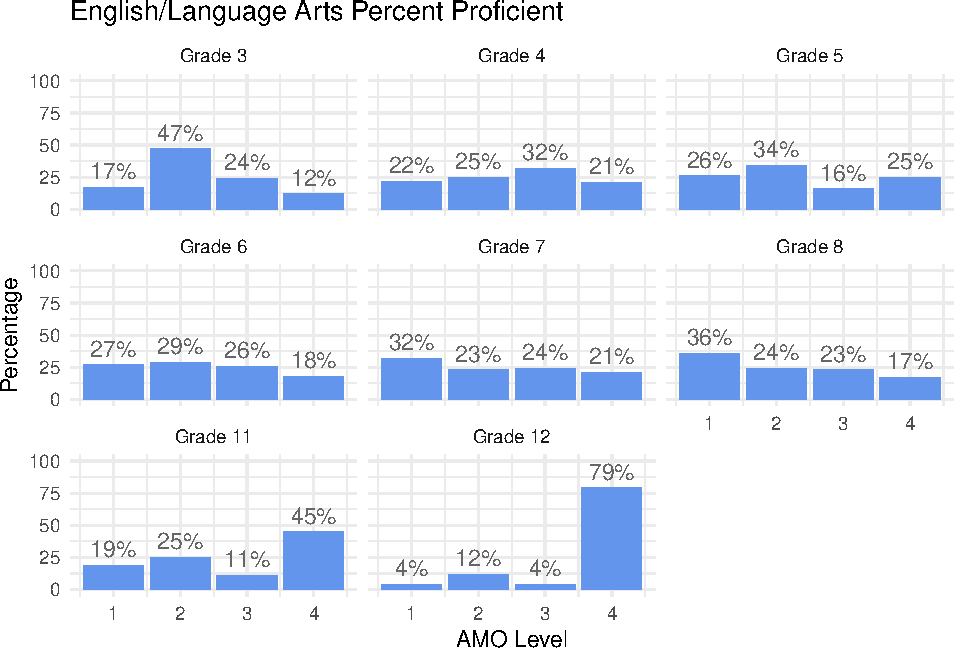
\includegraphics{tech_report_18_files/figure-latex/amo_plot-1.pdf}
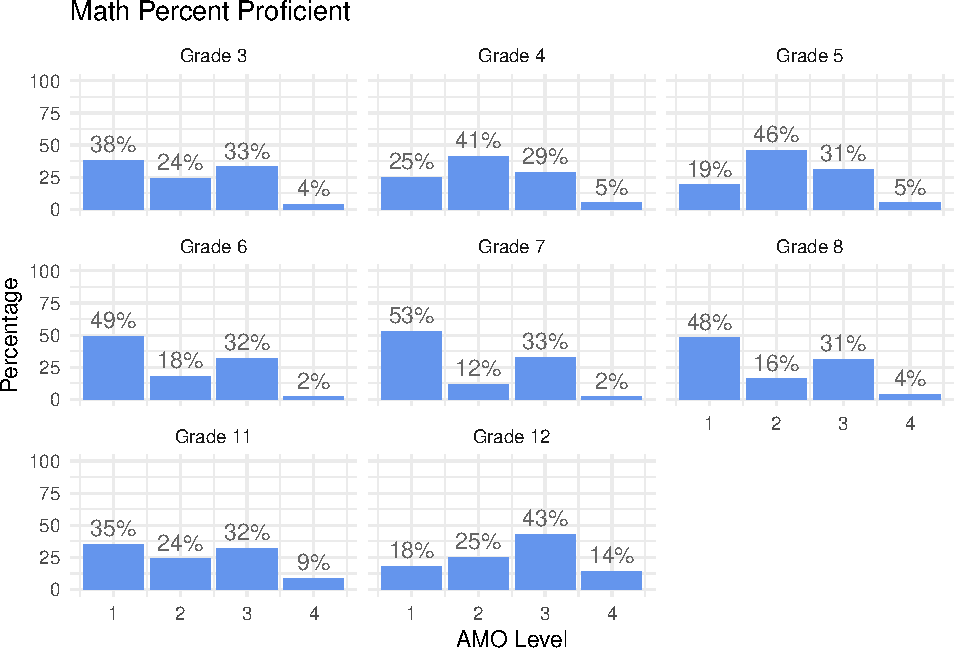
\includegraphics{tech_report_18_files/figure-latex/amo_plot-2.pdf}
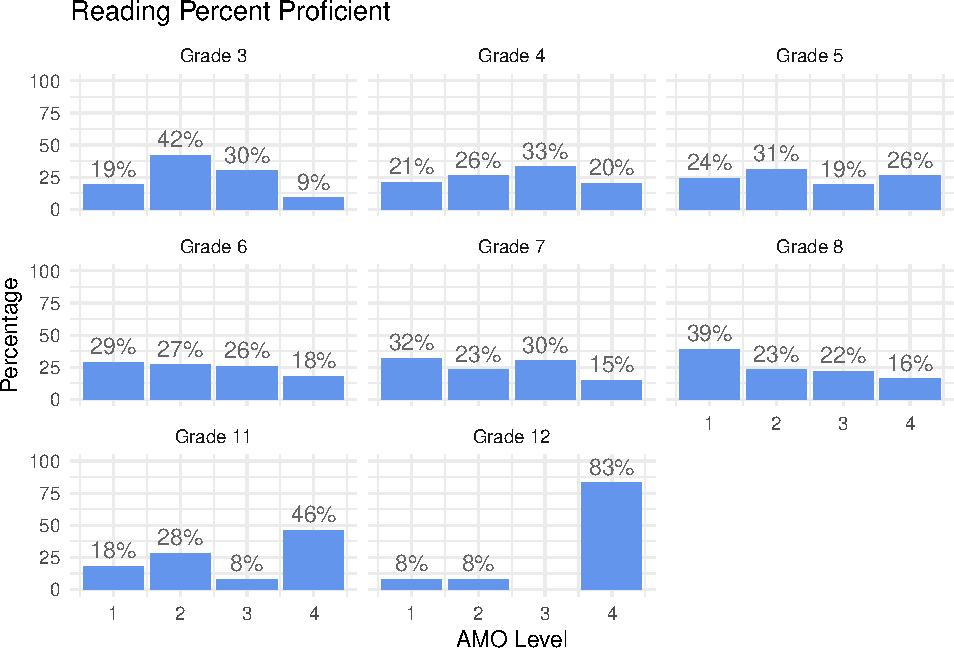
\includegraphics{tech_report_18_files/figure-latex/amo_plot-3.pdf}
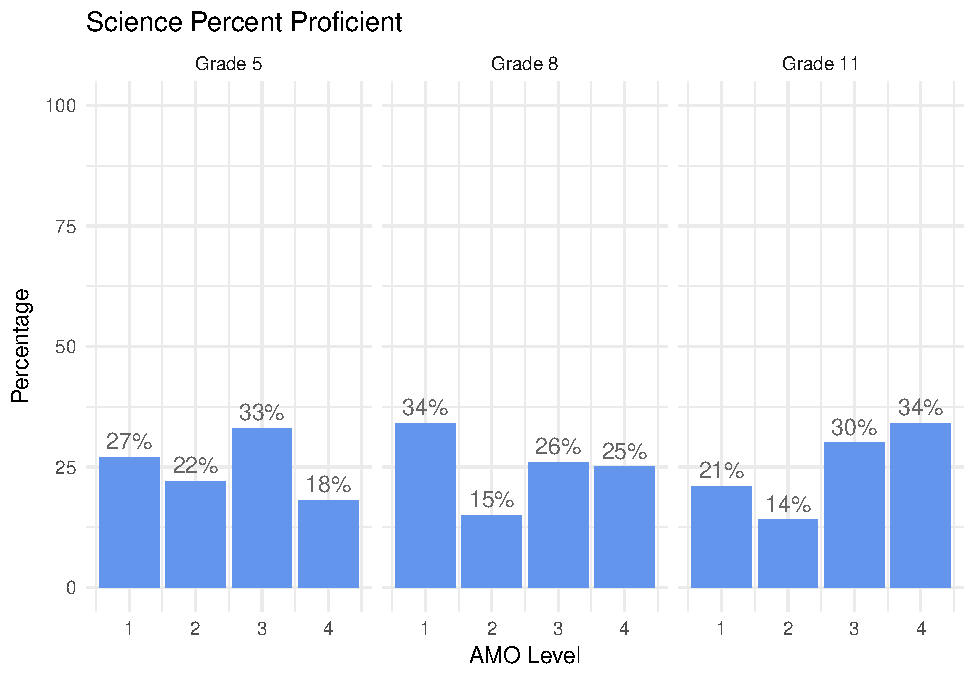
\includegraphics{tech_report_18_files/figure-latex/amo_plot-4.pdf}
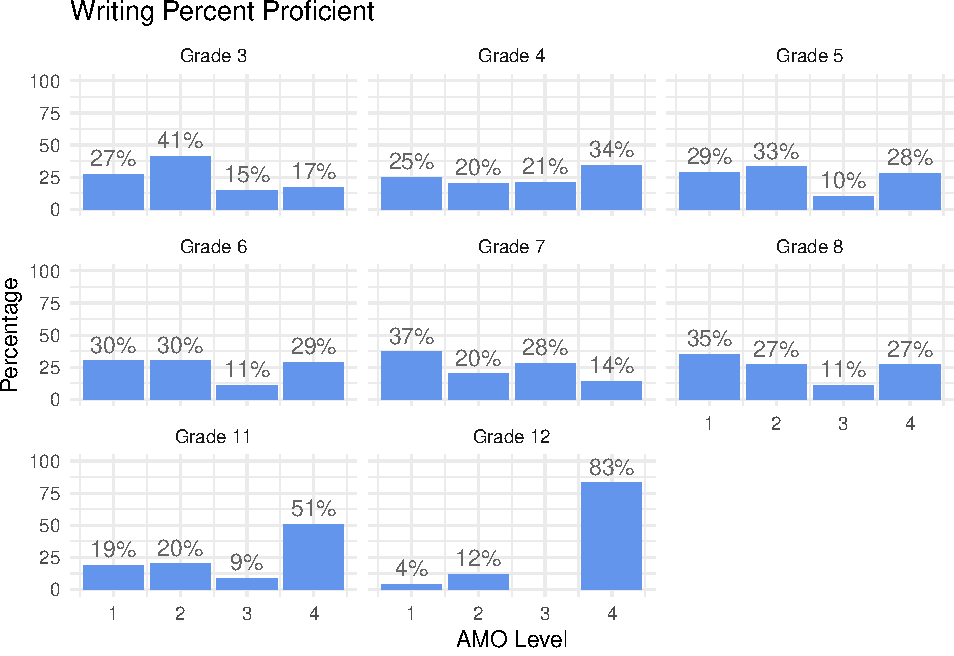
\includegraphics{tech_report_18_files/figure-latex/amo_plot-5.pdf}

Some concerns are noted in mathematics, where relatively higher
percentages of students are scoring at Level 1 and very few at Level 2.
However, this finding is consistent with the range of possible scores,
where Level 2 in some cases only has two possible scale score points
(e.g., Grade 7, where Level 2 exists between 207-208 scaled scores). The
addition of 1-2 low complexity items per assessment will be effected in
mathematics to address this concern, as well.

\subsubsection{3.4 Validity Based on Relations to Other
Variables}\label{validity-based-on-relations-to-other-variables}

Perhaps the best model for understanding criterion-related evidence
comes from Campbell and Fiske (1959) in their description of the
multi-trait, multi-method analysis {[}we translate the term `trait' to
mean `skill'{]}. In this process (several) different traits are measured
using (several) different methods to provide a correlation matrix that
should reflect specific patterns supportive of the claim being made
(that is, provide positive validation evidence). Sometimes, these
various measures are of the same or similar skills, abilities, or
traits, and other times they are of different skills, abilities, or
traits. We present data that quite consistently reflect higher relations
among items within an academic subject than between academic subjects.
We also present data in which performance on items is totaled within
categories of disability, expecting relations that would reflect
appropriate differences (see Tindal, McDonald, Tedesco, Glasgow, Almond,
Crawford, \& Hollenbeck, 2003).

\paragraph{Convergent and Divergent Validity
Documentation}\label{convergent-and-divergent-validity-documentation}

Criterion validity information is difficult to document with AA-AAAS, as
most SWSCD do not participate in any standardized assessment outside of
the ORExt and/or ORora in Oregon. Divergent validity evidence is
garnered via comparisons of ORExt results to ORora outcomes shows that
students whose ORExt assessments are discontinued exhibit serious
limitations in attention, basic math skills, and receptive and
expressive communication skills. The median ORExt ELA score for SWSCD
who participated in the ORora was 4.0. The median mathematics ORExt
score was 4.0, and the median science ORExt score for SWSCD who were
evaluated with the ORora was 0.0. Pearson correlations between the total
raw scores on the ORExt and the total raw score on the ORora were
conducted to address the relationship between total performance on each
assessment. The correlation between ELA and ORora scores was 0.56,
between Math and ORora scores was 0.52, and between Science and ORora
scores was 0.33. As expected, the ORora results provide divergent
validity evidence for the ORExt. We would not expect a strong
relationship between the scores, as students whose ORExt testing is
discontinued are generally unable to access the academic content on the
ORExt, even with the requisite reductions in depth, breadth, and
complexity.

Convergent evidence that the ORExt is assessing appropriate academic
content is provided by QA and QT responses to the consequential validity
survey. Respondents to the survey generally agree that, ``The items in
the Oregon Extended Assessment accurately reflect the academic content
(what the student should know) that my students with significant
cognitive disabilities should be learning, as defined by grade level
content standards (CCSS/NGSS) and the Essentialized Assessment
Frameworks'' (85\% Strongly Agree or Agree). In addition, they also
agreed with the statement that, ``The items in the Oregon Extended
Assessment, which primarily ask students to match, identify, or
recognize academic content, are appropriate behaviors to review to
determine what my students with significant cognitive disabilities are
able to do'' (85\% Strongly Agree or Agree). The consequential validity
results demonstrate that the ORExt is sampling academic domains that the
field of QAs and QTs deem appropriate in the area of academics. See
\emph{Appendix} 2.3B.10 for complete consequential vailidity study
results.

\paragraph{Analyses Within and Across Subject
Areas}\label{analyses-within-and-across-subject-areas}

We conducted correlational analyses to further explore the validity of
the ORExt. We first describe the purpose of the analysis, as well as our
anticipated results. We then discuss our observed results before
concluding with an overall evaluative judgment of the validity of the
test.

In the correlational analysis, we explore the correlations among
students' total scores across subject areas. The purpose of the analysis
was to investigate how strongly students' scores in one area were
related to students' scores in other subject areas. If the correlations
were exceedingly high (e.g., above .90), it would indicate that the
score a student receives in an individual subject has less to do with
the intended construct (i.e., reading) than with factors idiosyncratic
to the student. For example, if all subject areas correlated at .95,
then it would provide strong evidence that the tests would be measuring
a global student-specific construct (i.e., intelligence), and not the
individual subject constructs. We would expect, however, that the tests
would correlate quite strongly given that the same students were
assessed multiple times. Therefore, we would expect moderately strong
correlations (e.g., 0.7) simply because of the within-subject design.
Idiosyncratic variance associated with the individual student is thus
captured.

\paragraph{Correlational Analyses
Results}\label{correlational-analyses-results}

Full results of the Pearson's product-moment correlation analysis by
content area and grade level are reported below. The results are
significant, yet the overall correlations across content areas suggest
that we are indeed measuring different, though strongly related
constructs, with between-test scaled score correlations ranging from
0.69 to 0.97.

\FloatBarrier

\begin{table}[!h]

\caption{\label{tab:by_sub_corr}Grade 3 Content Area Correlations}
\centering
\begin{tabu} to \linewidth {>{\raggedright}X>{\raggedleft}X>{\raggedleft}X>{\raggedleft}X>{\raggedleft}X}
\toprule
Variable & ELA & Math & Reading & Writing\\
\midrule
ELA &  &  &  & \\
Math & 0.86 &  &  & \\
Reading & 0.96 & 0.83 &  & \\
Writing & 0.90 & 0.75 & 0.79 & \\
\bottomrule
\end{tabu}
\end{table}\begin{table}[!h]

\caption{\label{tab:by_sub_corr}Grade 4 Content Area Correlations}
\centering
\begin{tabu} to \linewidth {>{\raggedright}X>{\raggedleft}X>{\raggedleft}X>{\raggedleft}X>{\raggedleft}X}
\toprule
Variable & ELA & Math & Reading & Writing\\
\midrule
ELA &  &  &  & \\
Math & 0.79 &  &  & \\
Reading & 0.97 & 0.77 &  & \\
Writing & 0.92 & 0.73 & 0.84 & \\
\bottomrule
\end{tabu}
\end{table}\begin{table}[!h]

\caption{\label{tab:by_sub_corr}Grade 5 Content Area Correlations}
\centering
\begin{tabu} to \linewidth {>{\raggedright}X>{\raggedleft}X>{\raggedleft}X>{\raggedleft}X>{\raggedleft}X>{\raggedleft}X}
\toprule
Variable & ELA & Math & Reading & Science & Writing\\
\midrule
ELA &  &  &  &  & \\
Math & 0.82 &  &  &  & \\
Reading & 0.97 & 0.81 &  &  & \\
Science & 0.85 & 0.83 & 0.83 &  & \\
Writing & 0.94 & 0.75 & 0.87 & 0.79 & \\
\bottomrule
\end{tabu}
\end{table}\begin{table}[!h]

\caption{\label{tab:by_sub_corr}Grade 6 Content Area Correlations}
\centering
\begin{tabu} to \linewidth {>{\raggedright}X>{\raggedleft}X>{\raggedleft}X>{\raggedleft}X>{\raggedleft}X}
\toprule
Variable & ELA & Math & Reading & Writing\\
\midrule
ELA &  &  &  & \\
Math & 0.81 &  &  & \\
Reading & 0.97 & 0.80 &  & \\
Writing & 0.93 & 0.75 & 0.85 & \\
\bottomrule
\end{tabu}
\end{table}\begin{table}[!h]

\caption{\label{tab:by_sub_corr}Grade 7 Content Area Correlations}
\centering
\begin{tabu} to \linewidth {>{\raggedright}X>{\raggedleft}X>{\raggedleft}X>{\raggedleft}X>{\raggedleft}X}
\toprule
Variable & ELA & Math & Reading & Writing\\
\midrule
ELA &  &  &  & \\
Math & 0.76 &  &  & \\
Reading & 0.97 & 0.74 &  & \\
Writing & 0.93 & 0.69 & 0.84 & \\
\bottomrule
\end{tabu}
\end{table}\begin{table}[!h]

\caption{\label{tab:by_sub_corr}Grade 8 Content Area Correlations}
\centering
\begin{tabu} to \linewidth {>{\raggedright}X>{\raggedleft}X>{\raggedleft}X>{\raggedleft}X>{\raggedleft}X>{\raggedleft}X}
\toprule
Variable & ELA & Math & Reading & Science & Writing\\
\midrule
ELA &  &  &  &  & \\
Math & 0.77 &  &  &  & \\
Reading & 0.96 & 0.75 &  &  & \\
Science & 0.83 & 0.81 & 0.82 &  & \\
Writing & 0.94 & 0.74 & 0.87 & 0.79 & \\
\bottomrule
\end{tabu}
\end{table}\begin{table}[!h]

\caption{\label{tab:by_sub_corr}Grade 11 Content Area Correlations}
\centering
\begin{tabu} to \linewidth {>{\raggedright}X>{\raggedleft}X>{\raggedleft}X>{\raggedleft}X>{\raggedleft}X>{\raggedleft}X}
\toprule
Variable & ELA & Math & Reading & Science & Writing\\
\midrule
ELA &  &  &  &  & \\
Math & 0.85 &  &  &  & \\
Reading & 0.97 & 0.84 &  &  & \\
Science & 0.85 & 0.88 & 0.86 &  & \\
Writing & 0.94 & 0.78 & 0.87 & 0.79 & \\
\bottomrule
\end{tabu}
\end{table}\begin{table}[!h]

\caption{\label{tab:by_sub_corr}Grade 12 Content Area Correlations}
\centering
\begin{tabu} to \linewidth {>{\raggedright}X>{\raggedleft}X>{\raggedleft}X>{\raggedleft}X>{\raggedleft}X}
\toprule
Variable & ELA & Math & Reading & Writing\\
\midrule
ELA &  &  &  & \\
Math & 0.50 &  &  & \\
Reading & 0.95 & 0.50 &  & \\
Writing & 0.97 & 0.42 & 0.92 & \\
\bottomrule
\end{tabu}
\end{table}

\FloatBarrier

Results of the Pearson's product-moment correlation analysis within
English language arts (ELA:Reading:Writing) are reported below and
suggest high correlations between ELA and Reading, as expected, from .95
to .97. Writing is correlated with ELA from .90 to .94 and with reading
from .96 to .97.

The ORExt assessments appear to be measuring separate constructs, as
intended, indicated by the correlations. No unexpected and consistent
test functioning statistics are present based on student characteristics
that should not be related, such as gender and ethnicity. Student
performance appears to be primarily related to item difficulty and not
the result of construct irrelevant aspects that have been reviewed.

\subsection{Critical Element 4 - Technical Quality:
Other}\label{critical-element-4---technical-quality-other}

\subsubsection{4.1 Reliability}\label{reliability}

Test reliability can be viewed through several lenses, all of which
document how consistently an assessment performs across occasions,
contexts, and raters. Typical strategies for addressing reliability
include documentation of internal consistency, split-half reliability,
and test-retest reliability. If multiple forms are implemented, test
form reliability documentation is also requisite. The implementation
plan for the ORExt includes initial documentation of internal
consistency (Cronbach's alpha). The 2015-16 technical report included
internal consistency estimates, split-half reliability analyses, as well
as a small test-retest assessment of reliability comparisons by means of
our pilot tablet administration study. There is only one test form for
the ORExt, so test form comparisons are not possible.

\paragraph{Inter-Rater-Reliability}\label{inter-rater-reliability}

\subparagraph{Background}\label{background}

ODE's technical documentation plan (see page 136 in the 2016-17
Technical Report), included an Inter-Rater Reliability (IRR) study for
the 2017-18 school year. Pursuant to Hallgren, K. A. (2012) the
assessment of IRR may be necessary to demonstrate consistency among
observational ratings provided by multiple assessors. The results of the
study will be used to address the requirements within the USED's Peer
Review process (Critical Element 4.1). A sample of Oregon's Qualified
Assessors (QAs) who administer the paper/pencil version of the Oregon
Extended Assessment (ORExt) were observed to determine reliability of
administration and scoring. We did not include the tablet administration
or the Oregon Observational Rating.

\subparagraph{Methods}\label{methods}

QTs in districts across the state observe a sample of their respective
QAs using the observation protocol (see \emph{Appendix} 4.1
InterRater\_Observation\_Form) and enter their data online. The QA reads
the item stem and the student selects from three possible answer choices
(A, B, or C) then, the QA records the answer choice. QTs (observer)
records the students answer choice, then records the answer choice
recorded by the QA for agreement. Only the English Language Arts Writing
porting of the ORExt requires additional analysis by the assessor to
determine if the written response (answer) meets (1) or doesn't meet (0)
provided critera. Districts from across the state of Oregon participated
in the study, matching the state's student population demographics,
including large, medium, and small districts, across all regions. The
observation protocol was completed for the identified QA, but the
student(s) and content area(s) observed were selected by the QT or QA.
BRT researchers contacted district-level QTs at the beginning of the
test window, which runs from February 15 - April 26, 2018, to arrange
observations that could hopefully be completed within one school day. In
addition to addressing inter-rater reliability, the study also evaluated
test administration procedures. The methods, results, and interpretation
are provided here, in addition to recommended next steps. The
observation was composed of three sections:

\begin{itemize}
\item
  First, QT's reviewed ORExt paper/pencil test preparation and
  administration using the rubric (Appendix 4.1
  InterRater\_Observation\_Form). Test preparation/administration
  domains were rated on a four-point scale from Inappropriate (I) to
  Exemplary (E):

  \begin{itemize}
  \item
    Inappropriate (I) denotes a level of concern that could clearly
    affect the accuracy of the test results gathered from the test
    administration. Ratings at this level require substantive retraining
    of the QA involved.
  \item
    Somewhat Appropriate (SA) rating denotes a level that includes some
    minor aspects that could be improved, but the accuracy of the test
    results are likely not compromised.
  \item
    Appropriate (A) denotes a level that is consistent with all test
    administration requirements.
  \item
    Exemplary (E) level performance suggests that the QA incorporated
    approaches to test administration that could become models for best
    practice.
  \end{itemize}
\item
  Second, QT's scored the student alongside the QA using the scoring
  sheet. QT's compared results after this observation to ensure that the
  QA entered accurate data.
\item
  Finally, QT's observed the QA completing the data entry process to
  ensure that no errors are made during data entry and document the
  number of errors (Appendix 4.1 InterRater\_Observation\_Form).
\end{itemize}

Domain Definitions

\begin{enumerate}
\def\labelenumi{\arabic{enumi}.}
\item
  Test Security -- The QA utilized a system to ensure that all test
  materials were stored in a secure location,. The QA also had a
  district Assurance of Test Security form on file.
\item
  Printed Materials -- the QA had all materials required to administer
  the ORExt ready for test administration.
\item
  Distraction-Free Environment -- the QA arranged to provide the ORExt
  in a one-on-one test administration in a location that ensured that
  the student focused attention on the assessment.
\item
  Accessibility Supports -- the QA provided all necessary accessibility
  supports for the student and ensured that all support systems were
  functional prior to testing.
\item
  Level of Support -- The QA provided an appropriate level of support
  throughout testing that did not compromise the validity of the score.
\item
  Praise -- The QA utilized praise appropriately to support student
  involvement without leading the student to the correct answer.
\item
  Motivation -- The QA appropriately maintained the student's motivation
  during the assessment using relevant strategies, such as token
  systems.
\item
  Score Interpretation -- The QA demonstrated an appropriate
  understanding of how to use the cut scores and achievement level
  descriptors to interpret scores (i.e., ask the QA to describe how they
  interpret scores for parents).
\item
  Minimum Participation Rule - The QA demonstrated an appropriate
  understanding of the minimum participation rule (i.e., ask the QA to
  define the rule if it is not used).
\end{enumerate}

Qualified Assessor Testing Preparation and Administration Rubric (Record
an ``X'' in the cell that corresponds to your rating)

\FloatBarrier
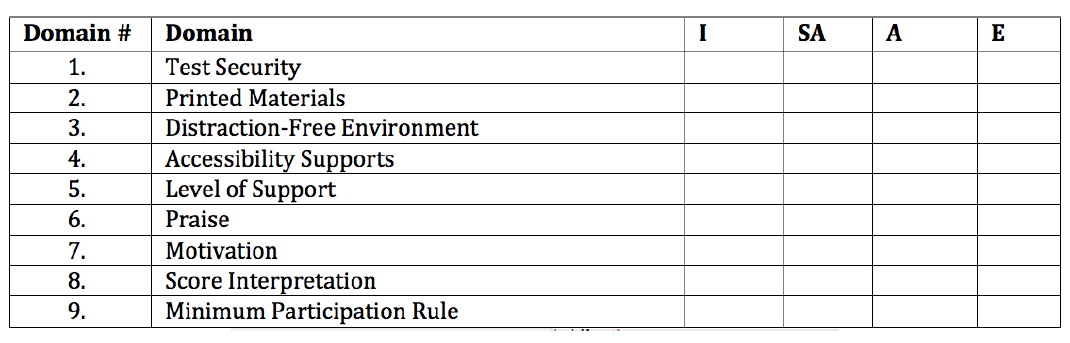
\includegraphics{Figures/irr/irr_domain.png}

\FloatBarrier

\subparagraph{Inter-rater Agreement
Results}\label{inter-rater-agreement-results}

Thirty-three Qualified Trainers from around Oregon participated in the
Inter-Rater-Reliability study by doing at least one observation on the
Oregon Extended Assessment via paper/pencil administration. Of the
thirty-three observations, 48.5\% were English Language Arts, 33.3\%
were Mathematics, and 18.2\% were Science. Observations were done at
individual student's typical testing location. The study found a 99.3
Inter-Rater Reliability percentage agreement between the test observers
and test administrators on student item (answer) selection.

The following two tables (Table 21 and Table 22) display the percentage
of reponses in the nine different domains and percentage of agreement
between assessors and observers.\\
\FloatBarrier

\begin{table}[!h]

\caption{\label{tab:unnamed-chunk-1}Percentage for responses}
\centering
\begin{tabu} to \linewidth {>{\raggedright}X>{\raggedleft}X>{\raggedleft}X>{\raggedleft}X>{\raggedleft}X}
\toprule
var & Exemplary & Appropriate & Somewhat Appropriate & Inappropriate\\
\midrule
accessibility\_supports & 40 & 56 & 4 & 0\\
distraction\_free & 28 & 72 & 0 & 0\\
level\_support & 52 & 48 & 0 & 0\\
minimum\_participation & 48 & 48 & 4 & 0\\
motivation & 44 & 56 & 0 & 0\\
\addlinespace
praise & 60 & 40 & 0 & 0\\
printed\_materials & 56 & 44 & 0 & 0\\
score\_interpretation & 28 & 48 & 16 & 8\\
test\_security & 56 & 40 & 4 & 0\\
\bottomrule
\end{tabu}
\end{table}

\begin{table}[!h]

\caption{\label{tab:unnamed-chunk-1}Mark As Disagree}
\centering
\begin{tabu} to \linewidth {>{\raggedright}X>{\raggedleft}X>{\raggedleft}X>{\raggedleft}X}
\toprule
response & n & tot & percent\\
\midrule
0 & 310 & 1200 & 25.83\\
1 & 645 & 1200 & 53.75\\
1, Mark As Disagree & 1 & 1200 & 0.08\\
Not Administered & 244 & 1200 & 20.33\\
\bottomrule
\end{tabu}
\end{table}

\clearpage
\FloatBarrier
The following table provides a visual display of the responses from the
nine differnt domains observed.

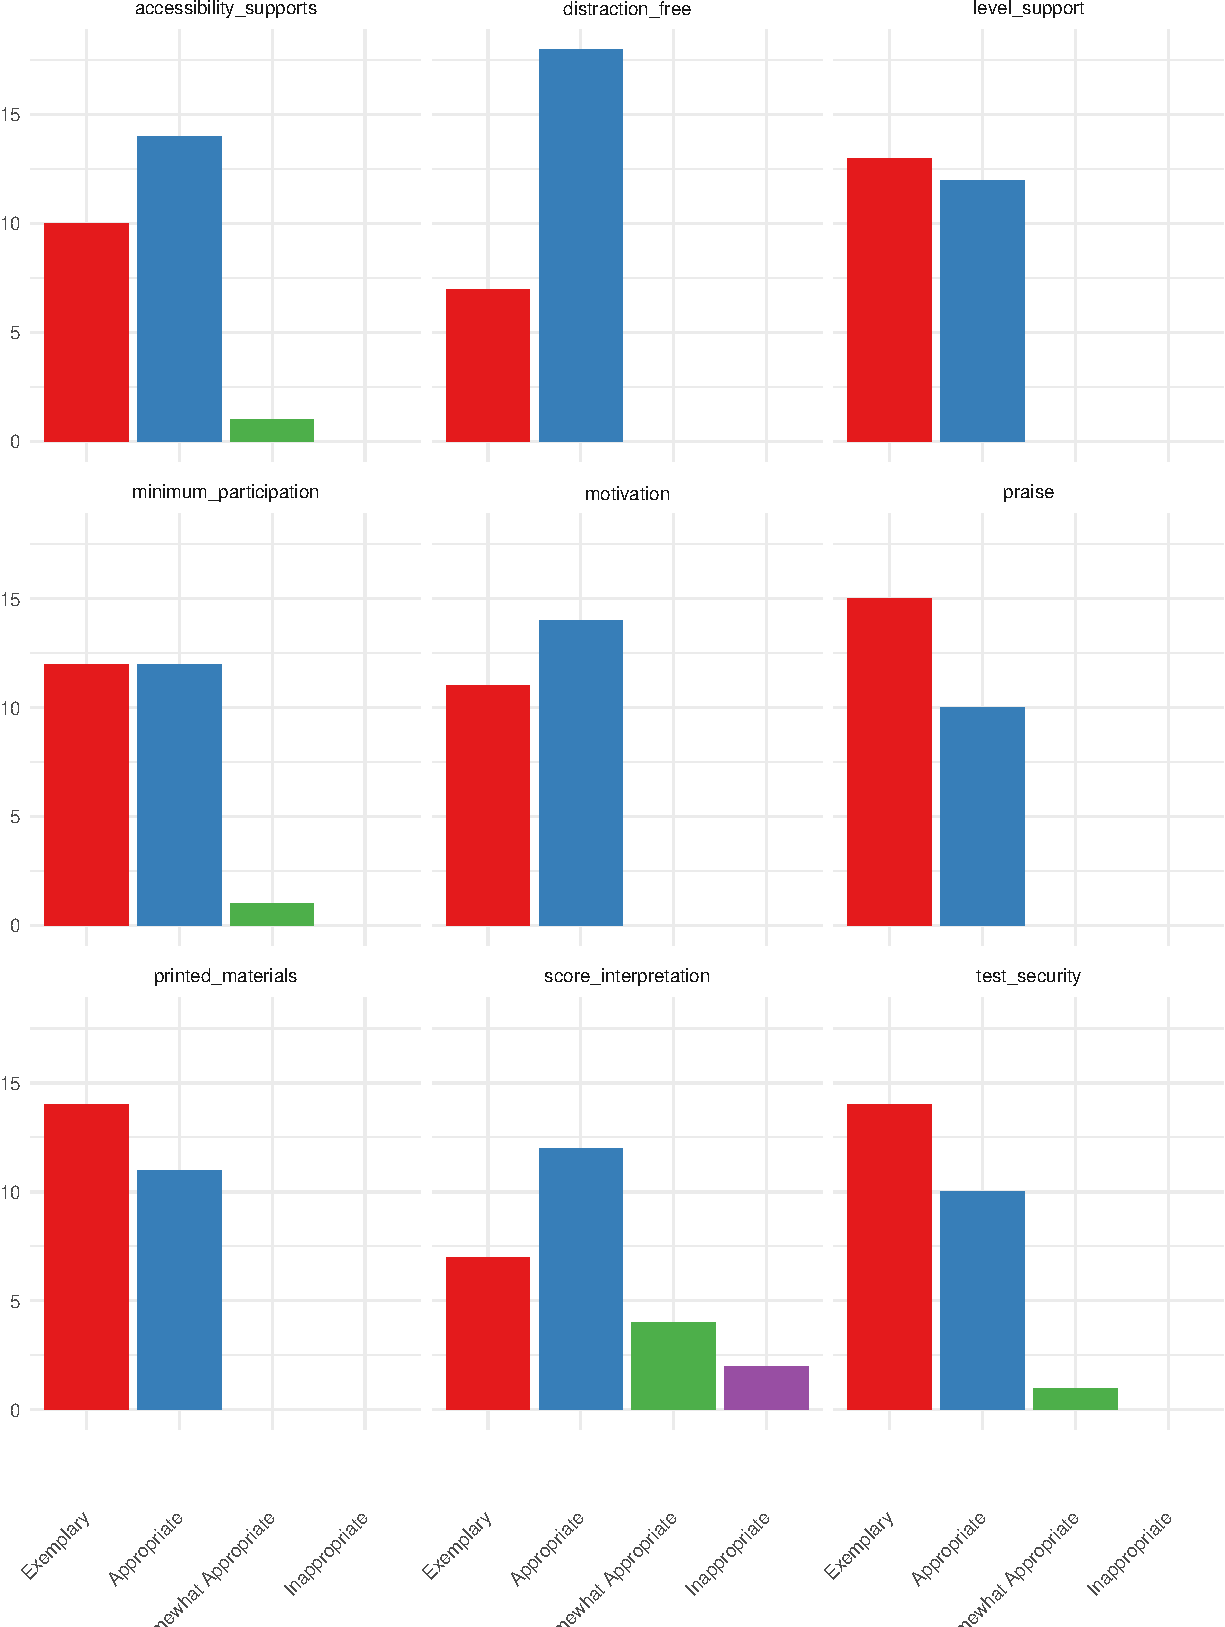
\includegraphics{tech_report_18_files/figure-latex/unnamed-chunk-2-1.pdf}
Interpretation: Provide an interpretation of the results above here.

Next Steps and Recommendations: Give ODE action steps to pursue in any
areas of concern (writing scoring accuracy/exemplars and score
interpretation training)

\clearpage
\#\#\#\# 4.1A Test Reliability

\subparagraph{4.1A Test Reliability}\label{a-test-reliability}

Marginal reliability results (true score variance/true score variance +
error variance) demonstrate that the tests are quite reliable at the
total test level. Full reliability statistics for each of the
operational tests administered this year are provided below. These
results demonstrate that the total test reliabilities were quite high,
ranging from .67 to .91. Each table below provides the content area,
grade, and the marginal reliabilities. All test forms were composed of
36 operational and 12 embedded field-test items.

\begin{table}[!h]

\caption{\label{tab:marginal_rel}ELA Marginal Reliabilities}
\centering
\begin{tabu} to \linewidth {>{\raggedleft}X>{\raggedleft}X}
\toprule
Grade & Marginal Reliability Estimate\\
\midrule
3 & 0.91\\
4 & 0.91\\
5 & 0.91\\
6 & 0.91\\
7 & 0.91\\
\addlinespace
8 & 0.91\\
11 & 0.90\\
12 & 0.80\\
\bottomrule
\end{tabu}
\end{table}\begin{table}[!h]

\caption{\label{tab:marginal_rel}Math Marginal Reliabilities}
\centering
\begin{tabu} to \linewidth {>{\raggedleft}X>{\raggedleft}X}
\toprule
Grade & Marginal Reliability Estimate\\
\midrule
3 & 0.90\\
4 & 0.90\\
5 & 0.88\\
6 & 0.88\\
7 & 0.89\\
\addlinespace
8 & 0.87\\
11 & 0.89\\
12 & 0.89\\
\bottomrule
\end{tabu}
\end{table}\begin{table}[!h]

\caption{\label{tab:marginal_rel}Reading Marginal Reliabilities}
\centering
\begin{tabu} to \linewidth {>{\raggedleft}X>{\raggedleft}X}
\toprule
Grade & Marginal Reliability Estimate\\
\midrule
3 & 0.86\\
4 & 0.86\\
5 & 0.86\\
6 & 0.85\\
7 & 0.86\\
\addlinespace
8 & 0.84\\
11 & 0.83\\
12 & 0.69\\
\bottomrule
\end{tabu}
\end{table}\begin{table}[!h]

\caption{\label{tab:marginal_rel}Science Marginal Reliabilities}
\centering
\begin{tabu} to \linewidth {>{\raggedleft}X>{\raggedleft}X}
\toprule
Grade & Marginal Reliability Estimate\\
\midrule
5 & 0.91\\
8 & 0.90\\
11 & 0.88\\
\bottomrule
\end{tabu}
\end{table}\begin{table}[!h]

\caption{\label{tab:marginal_rel}Writing Marginal Reliabilities}
\centering
\begin{tabu} to \linewidth {>{\raggedleft}X>{\raggedleft}X}
\toprule
Grade & Marginal Reliability Estimate\\
\midrule
3 & 0.82\\
4 & 0.81\\
5 & 0.82\\
6 & 0.81\\
7 & 0.82\\
\addlinespace
8 & 0.81\\
11 & 0.82\\
12 & 0.67\\
\bottomrule
\end{tabu}
\end{table}

\clearpage

\subsubsection{Test Information
Functions}\label{test-information-functions}

The test information functions published below also indicate that the
scales exhibit a reliability greater than or equal to .80 for all
proficient-level cutscores.

\subsubsection{English Language Arts
TIFs}\label{english-language-arts-tifs}

\FloatBarrier
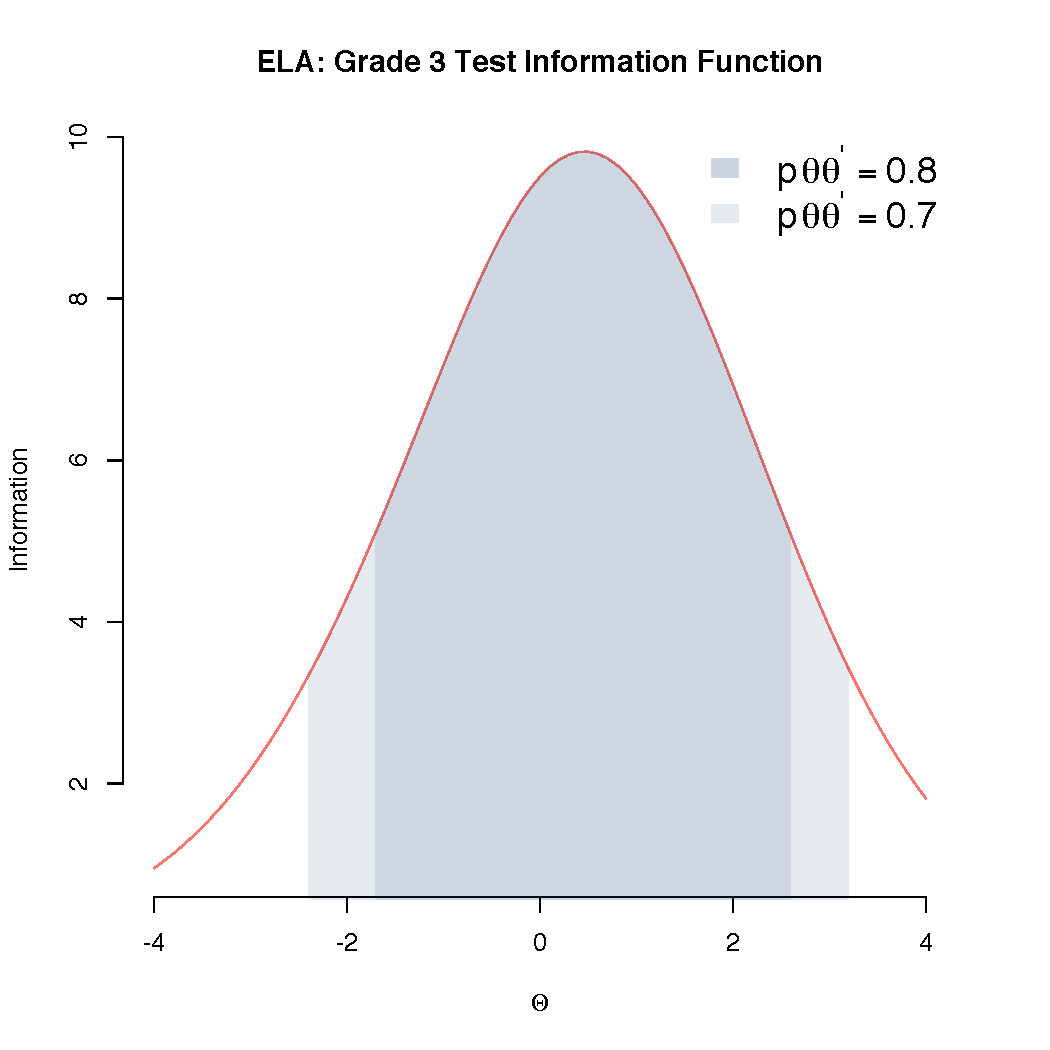
\includegraphics[height=3.12500in]{tifs/ela3tif.pdf}
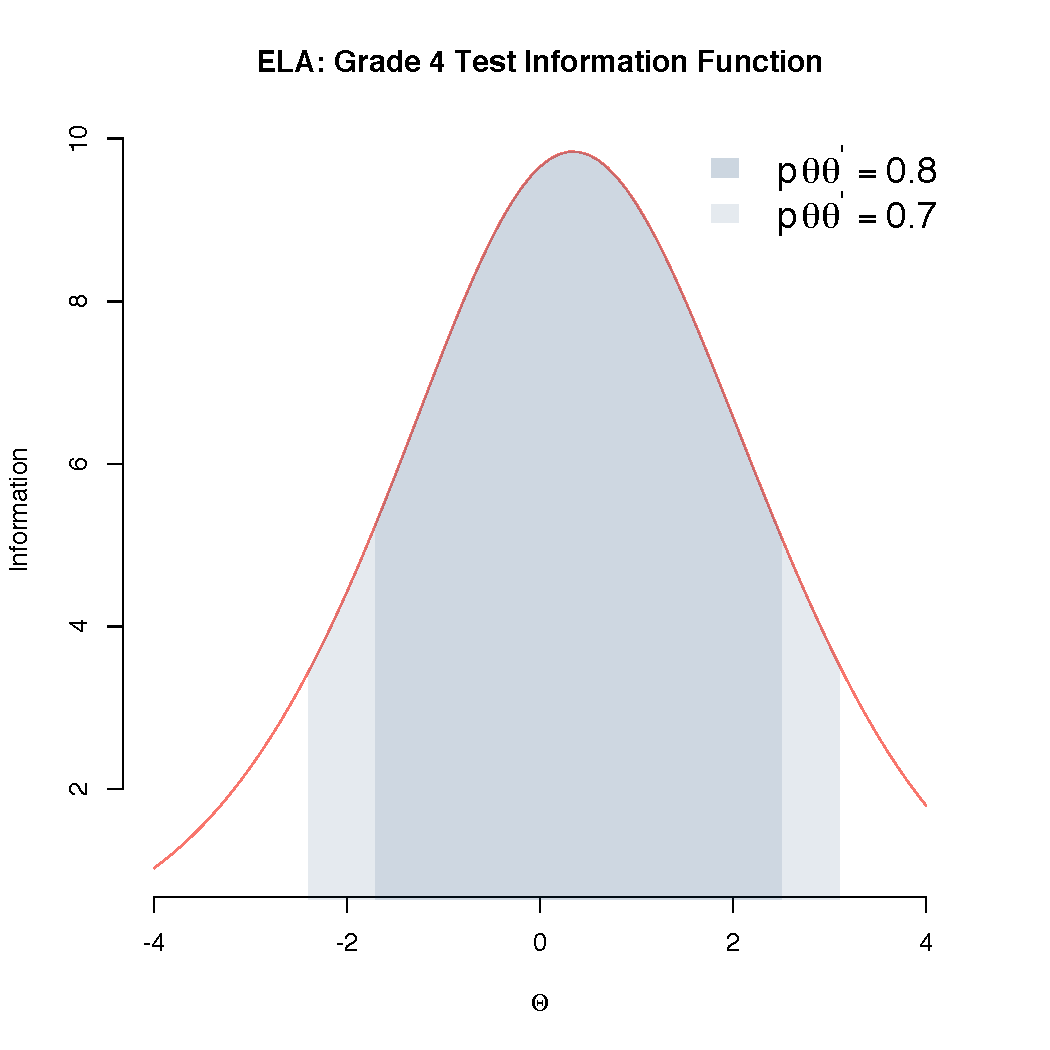
\includegraphics[height=3.12500in]{tifs/ela4tif.pdf}
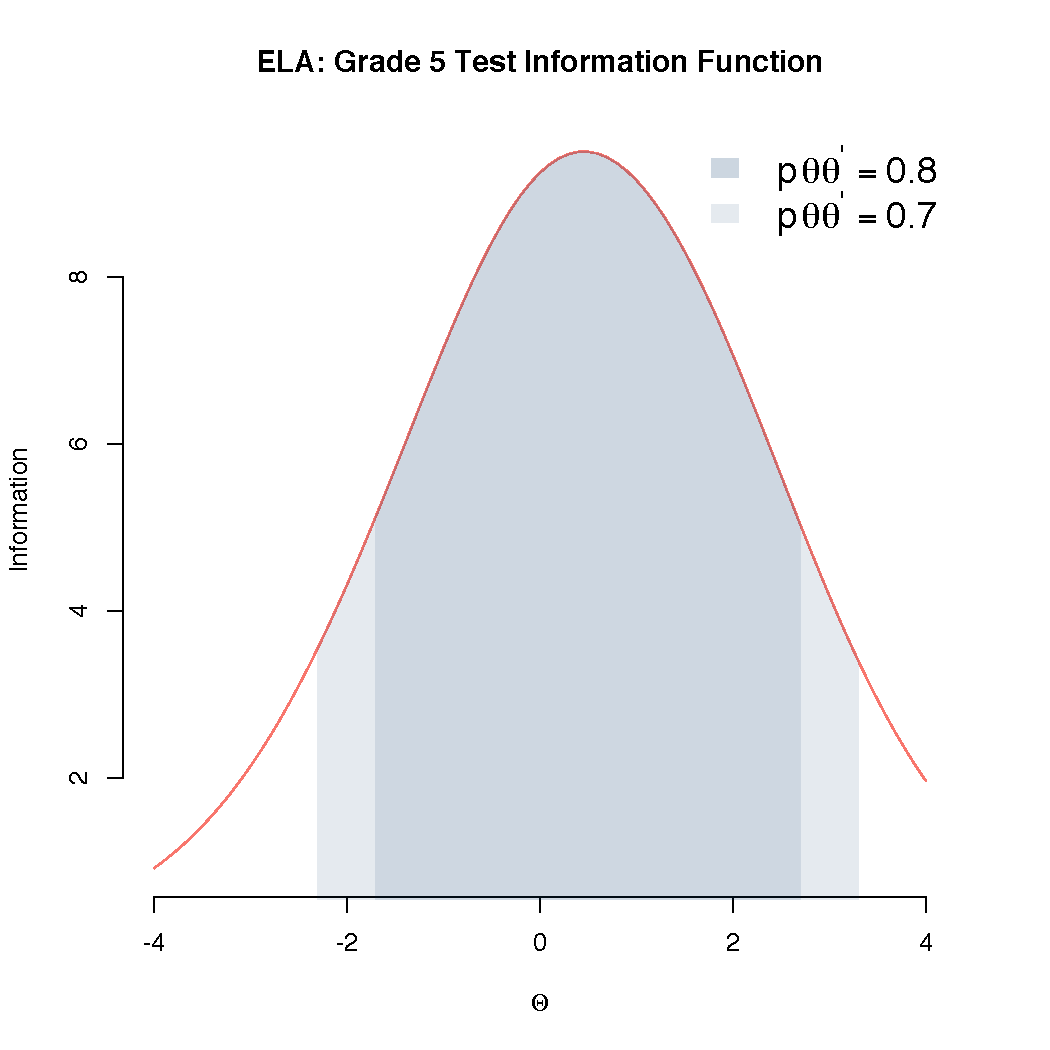
\includegraphics[height=3.12500in]{tifs/ela5tif.pdf}
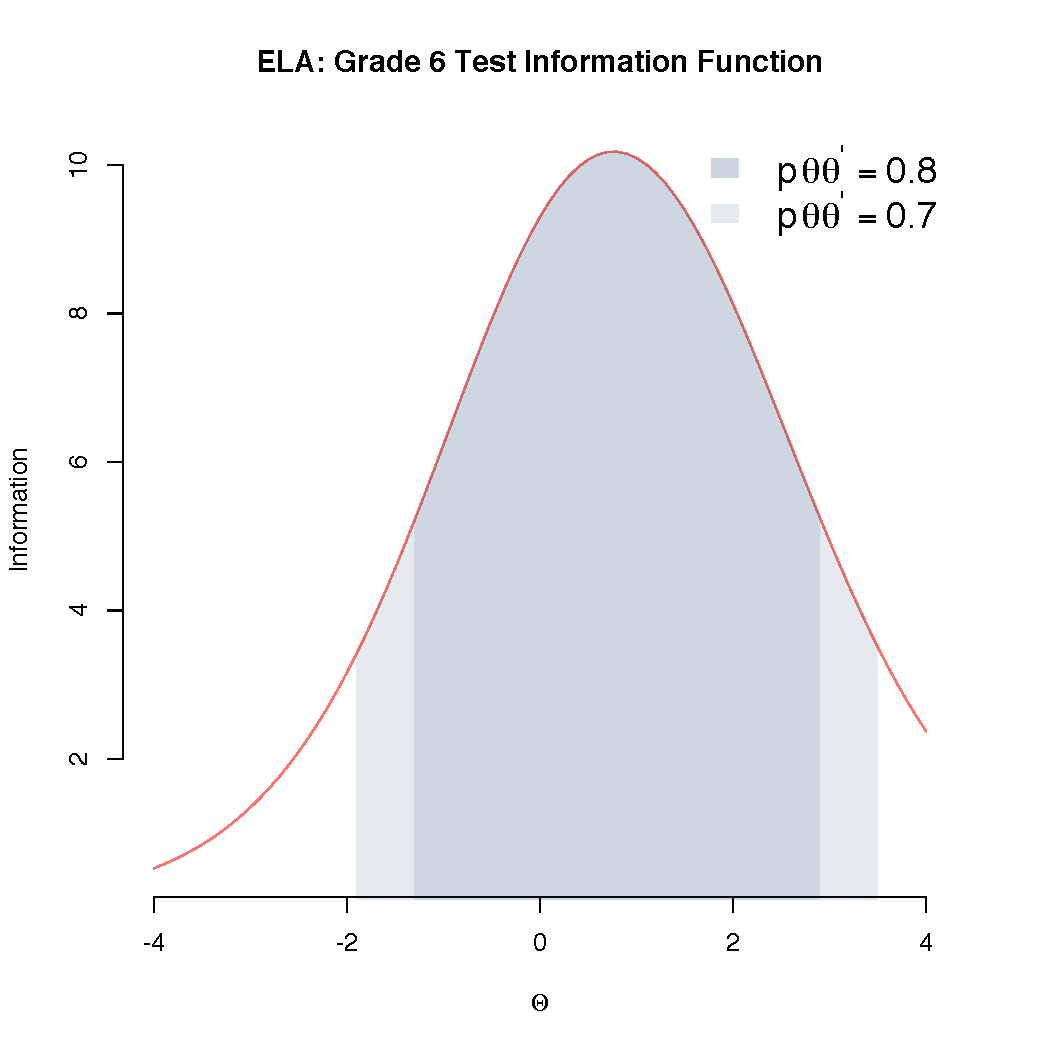
\includegraphics[height=3.12500in]{tifs/ela6tif.pdf}
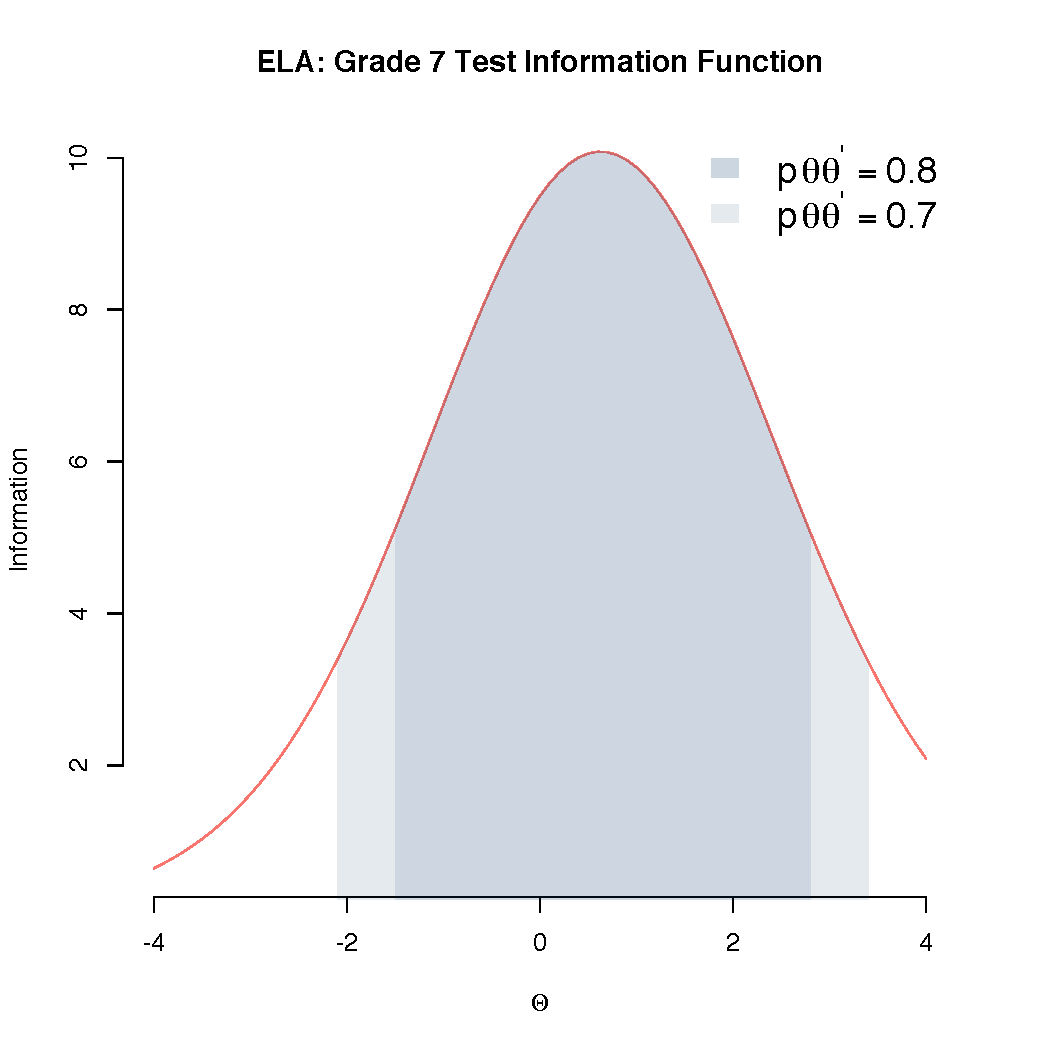
\includegraphics[height=3.12500in]{tifs/ela7tif.pdf}
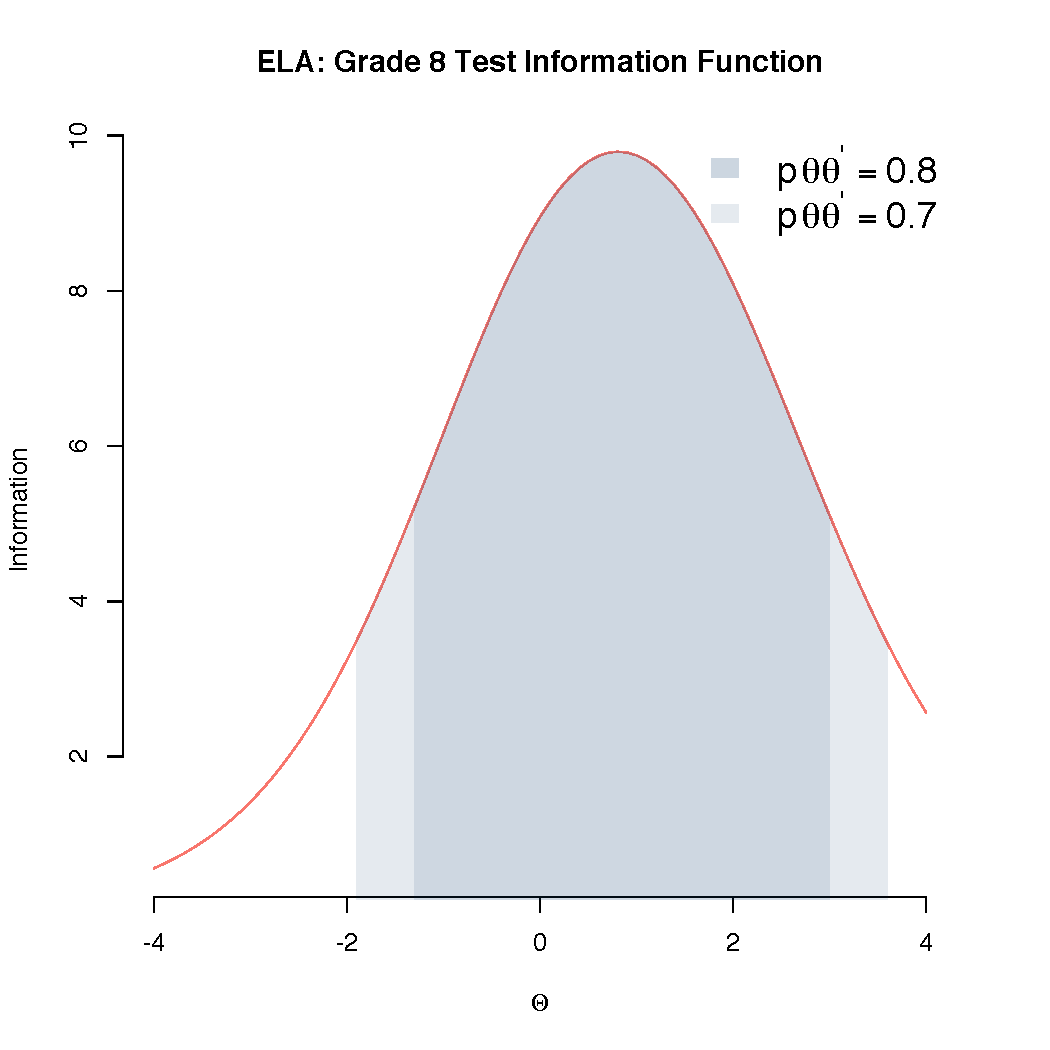
\includegraphics[height=3.12500in]{tifs/ela8tif.pdf}
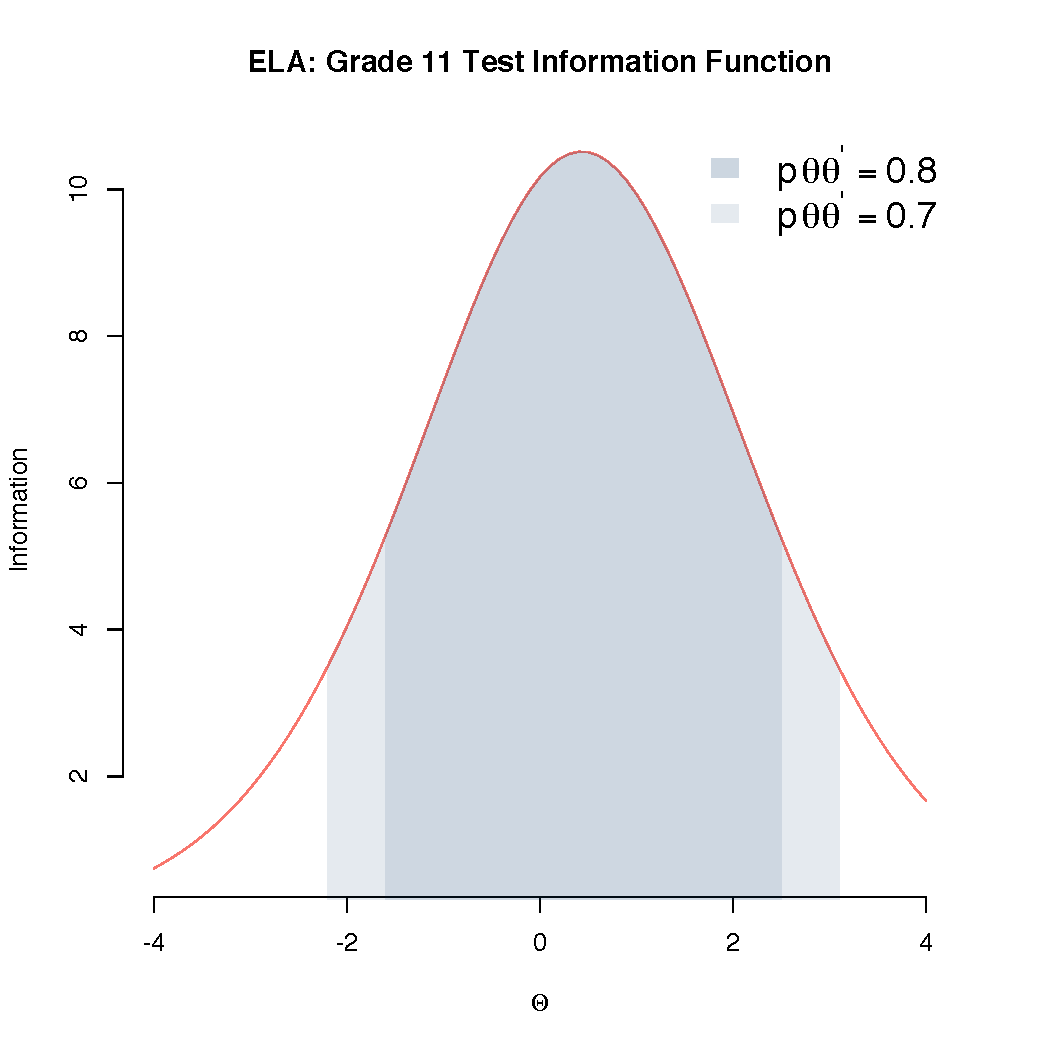
\includegraphics[height=3.12500in]{tifs/ela11tif.pdf}

\subsubsection{Mathematics TIFs}\label{mathematics-tifs}

\FloatBarrier
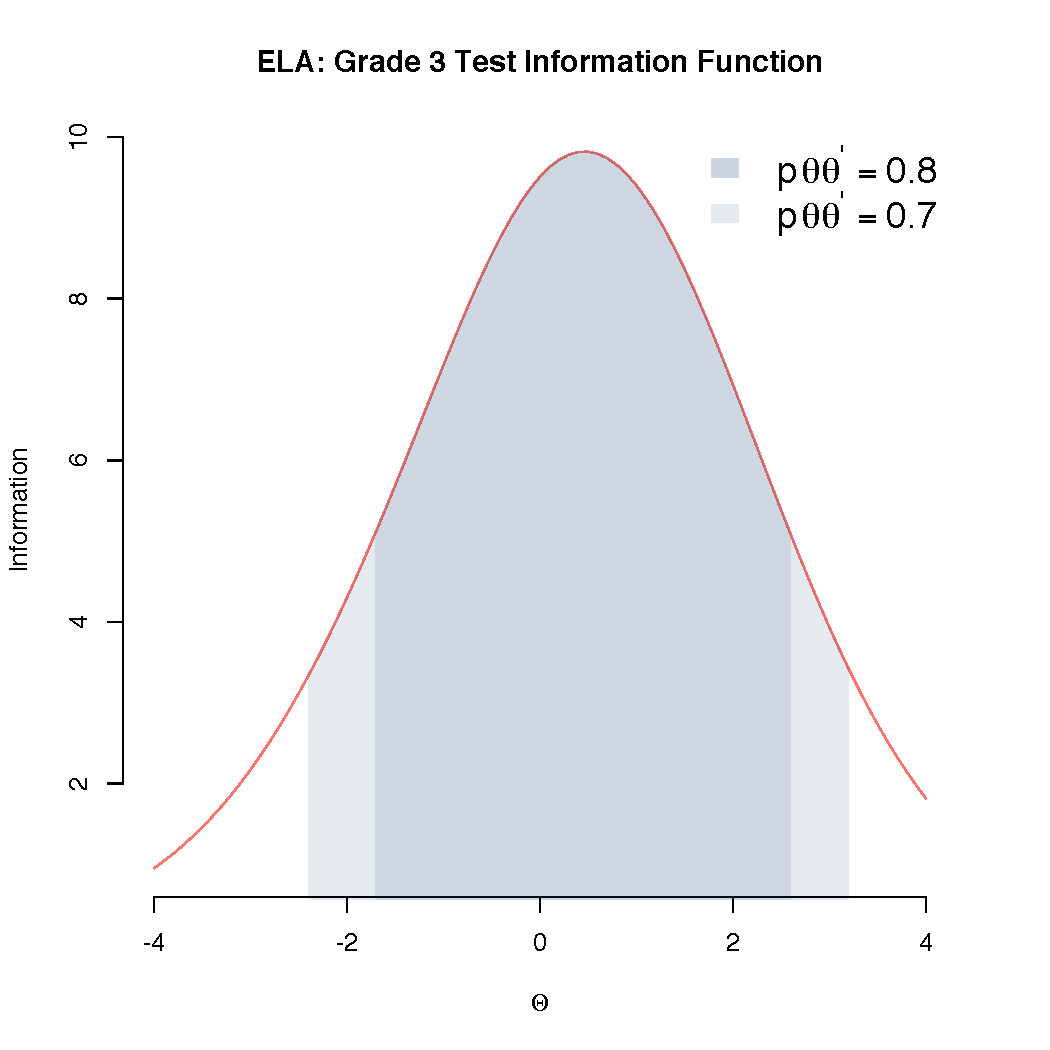
\includegraphics[height=3.12500in]{tifs/ela3tif.pdf}
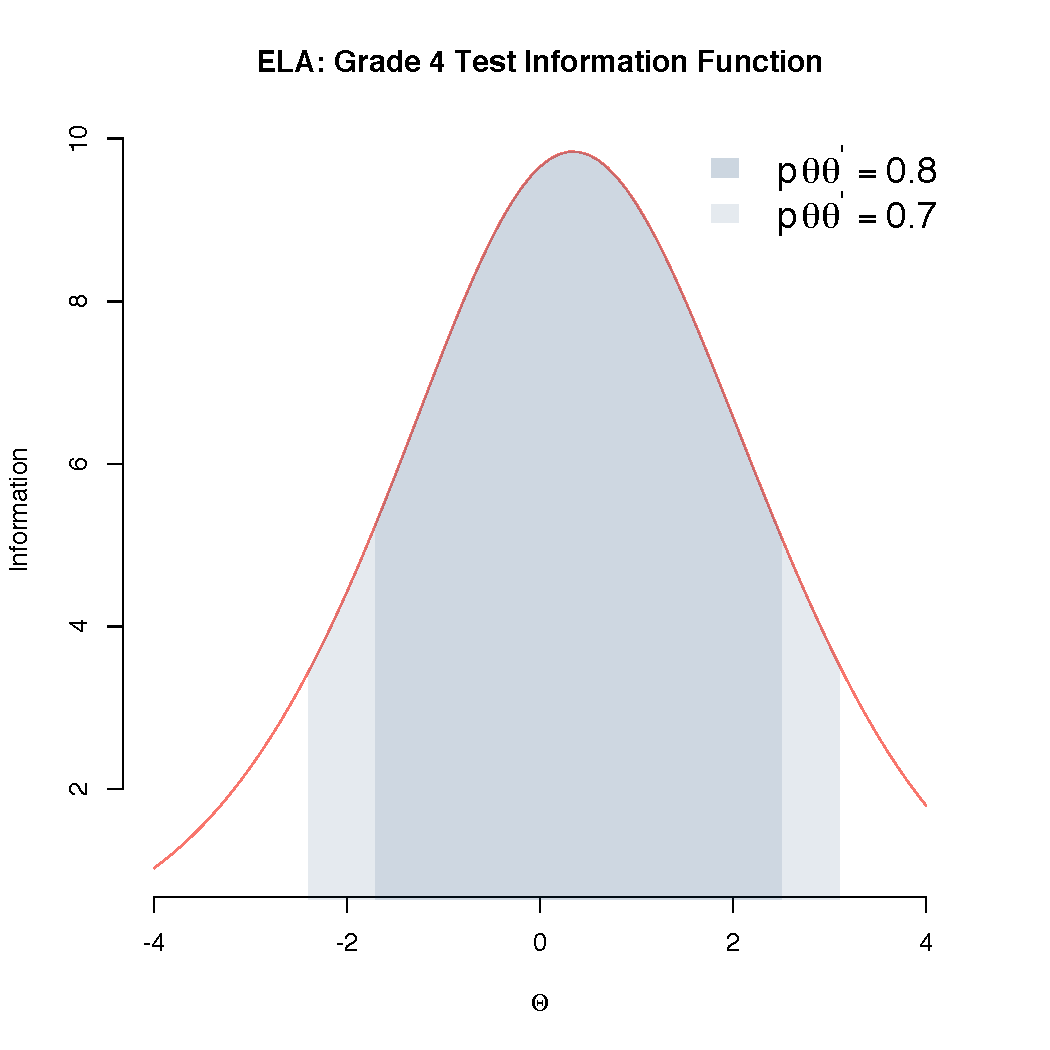
\includegraphics[height=3.12500in]{tifs/ela4tif.pdf}
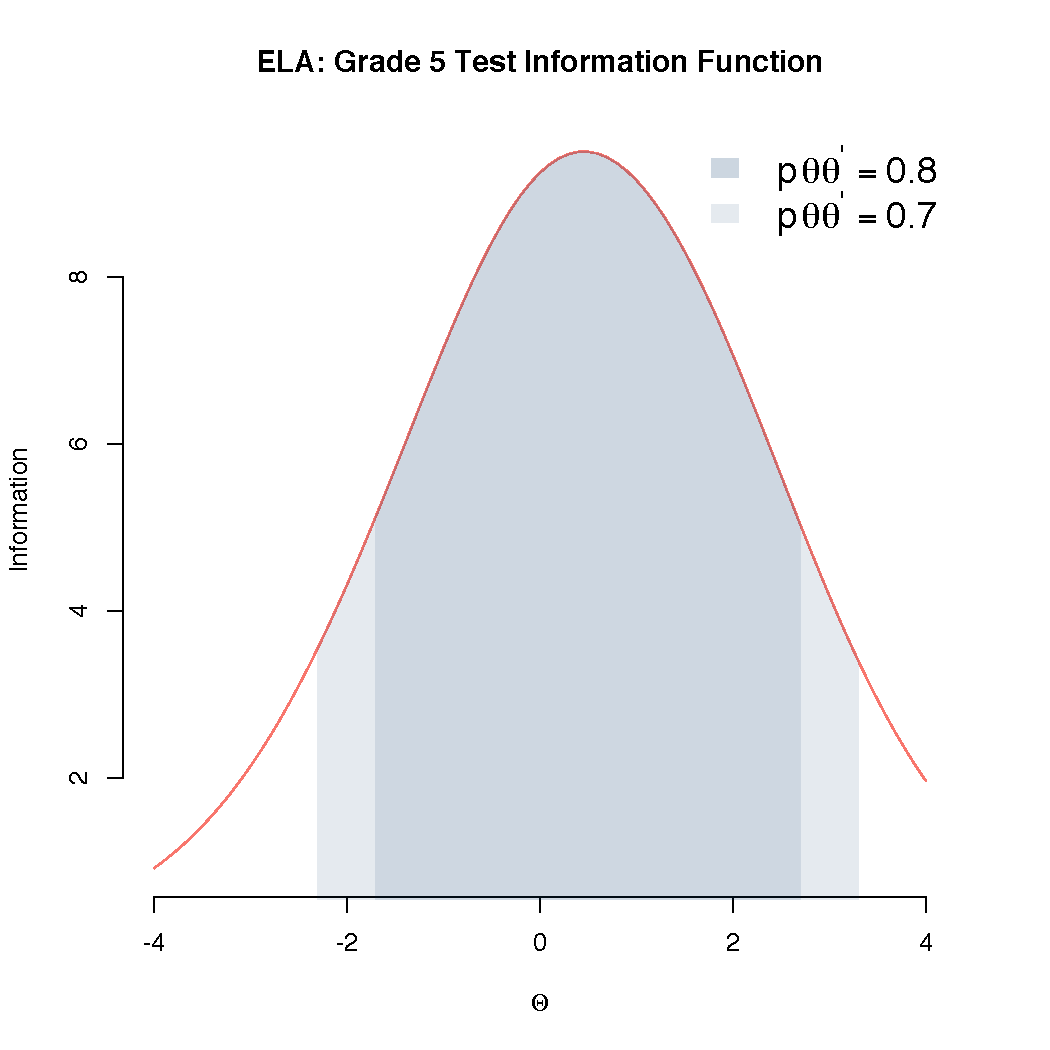
\includegraphics[height=3.12500in]{tifs/ela5tif.pdf}
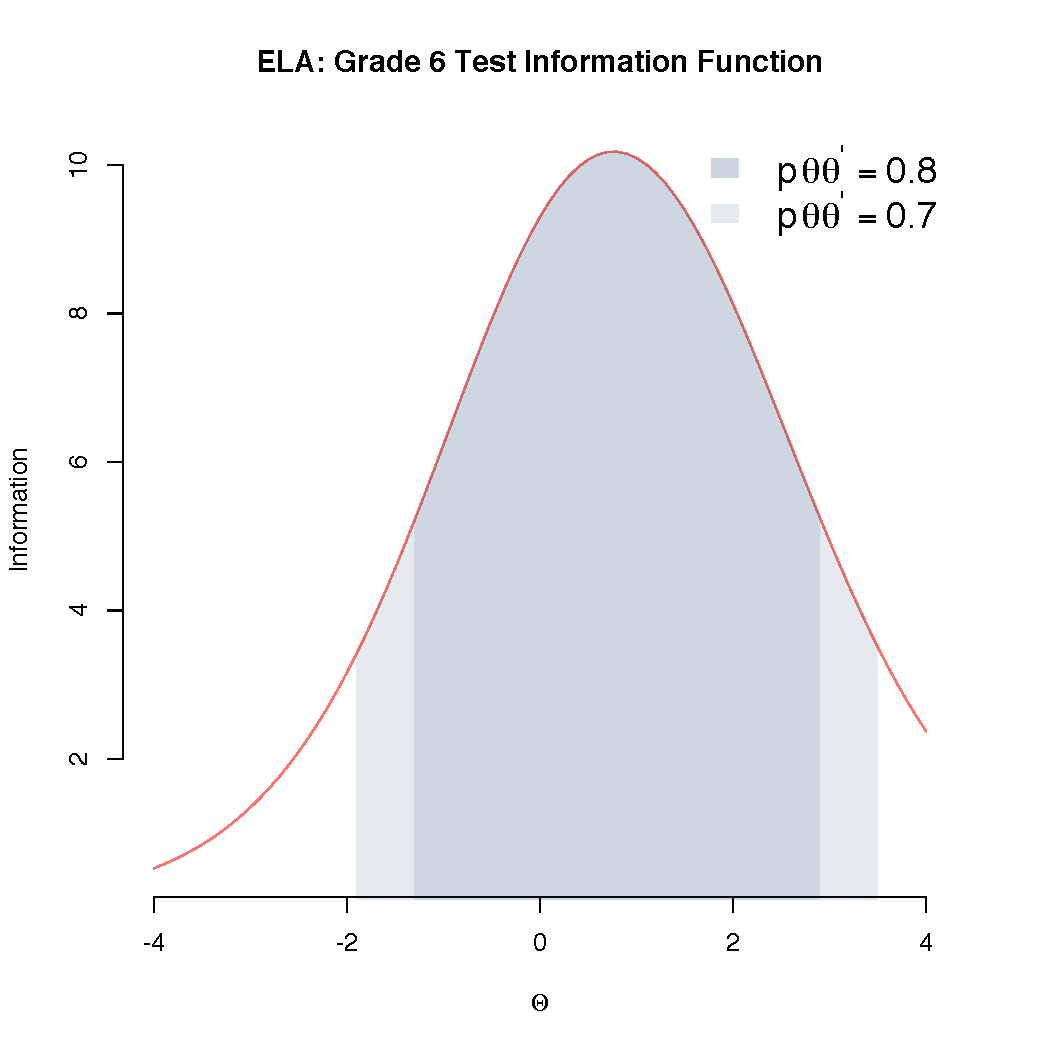
\includegraphics[height=3.12500in]{tifs/ela6tif.pdf}
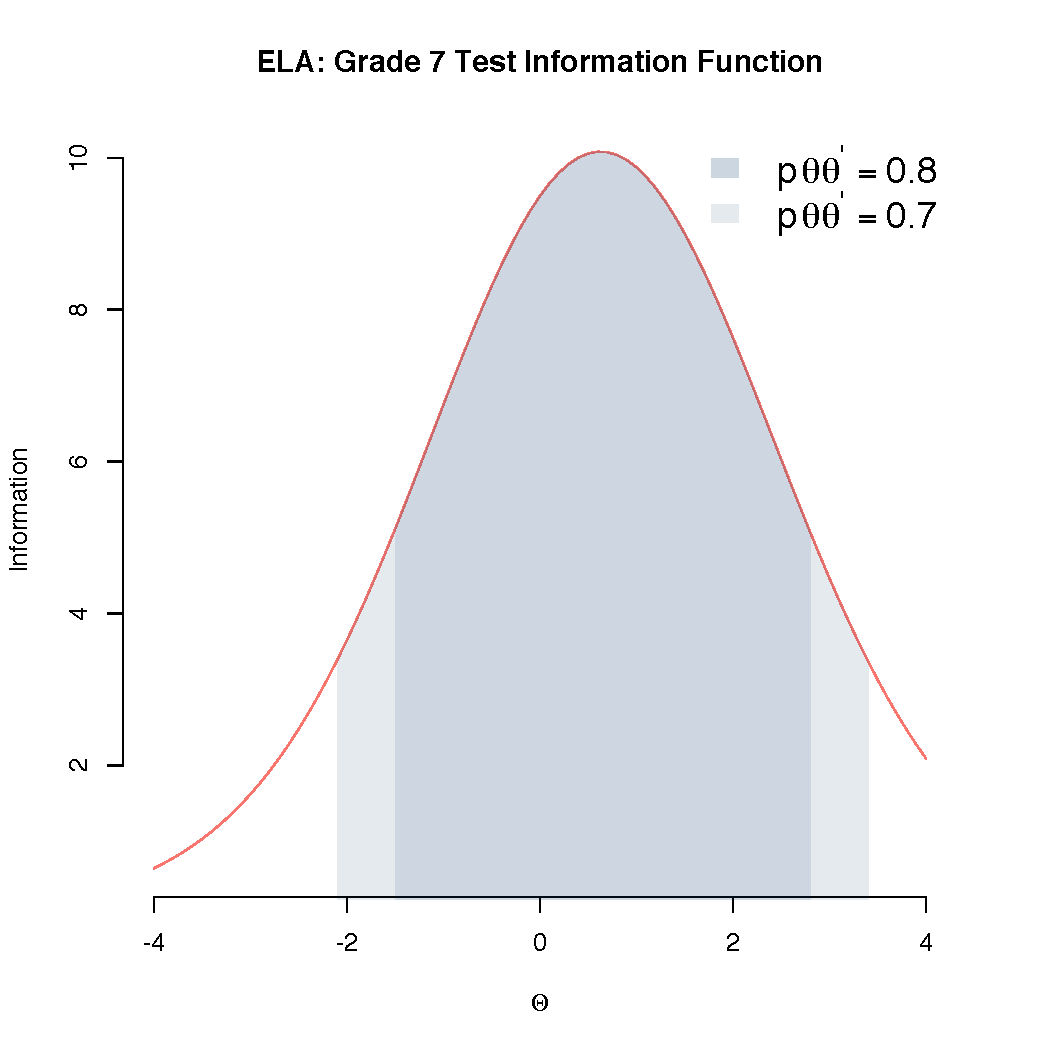
\includegraphics[height=3.12500in]{tifs/ela7tif.pdf}
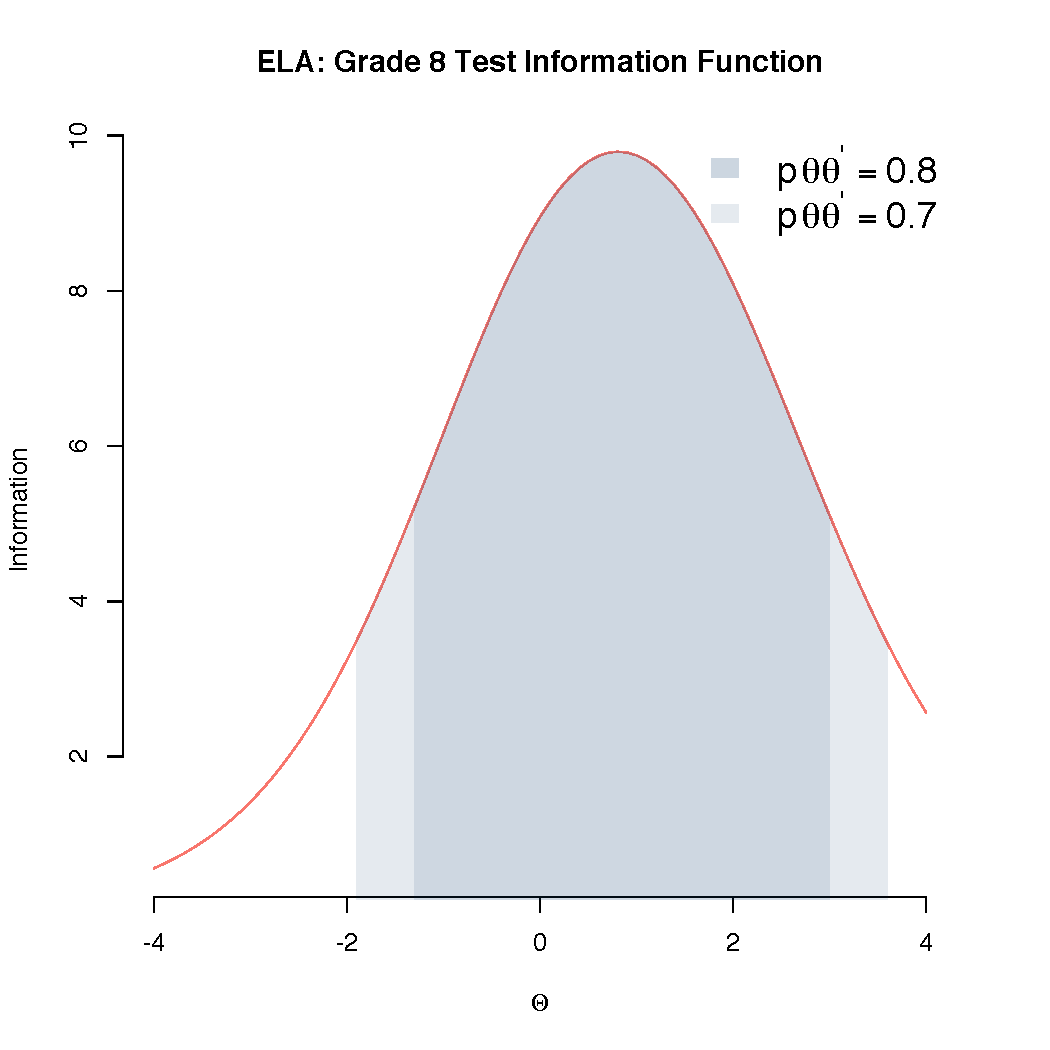
\includegraphics[height=3.12500in]{tifs/ela8tif.pdf}
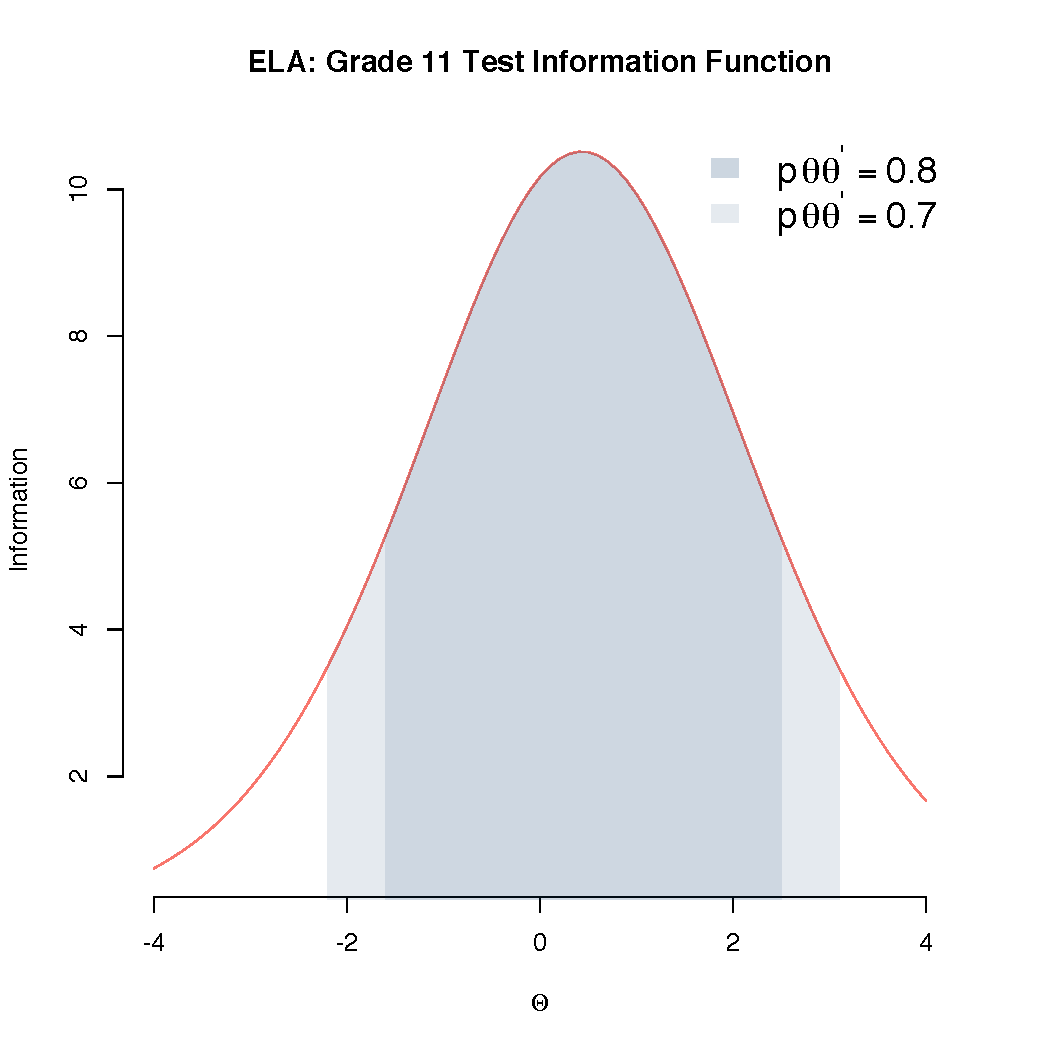
\includegraphics[height=3.12500in]{tifs/ela11tif.pdf}

\subsubsection{Science TIFs}\label{science-tifs}

\FloatBarrier
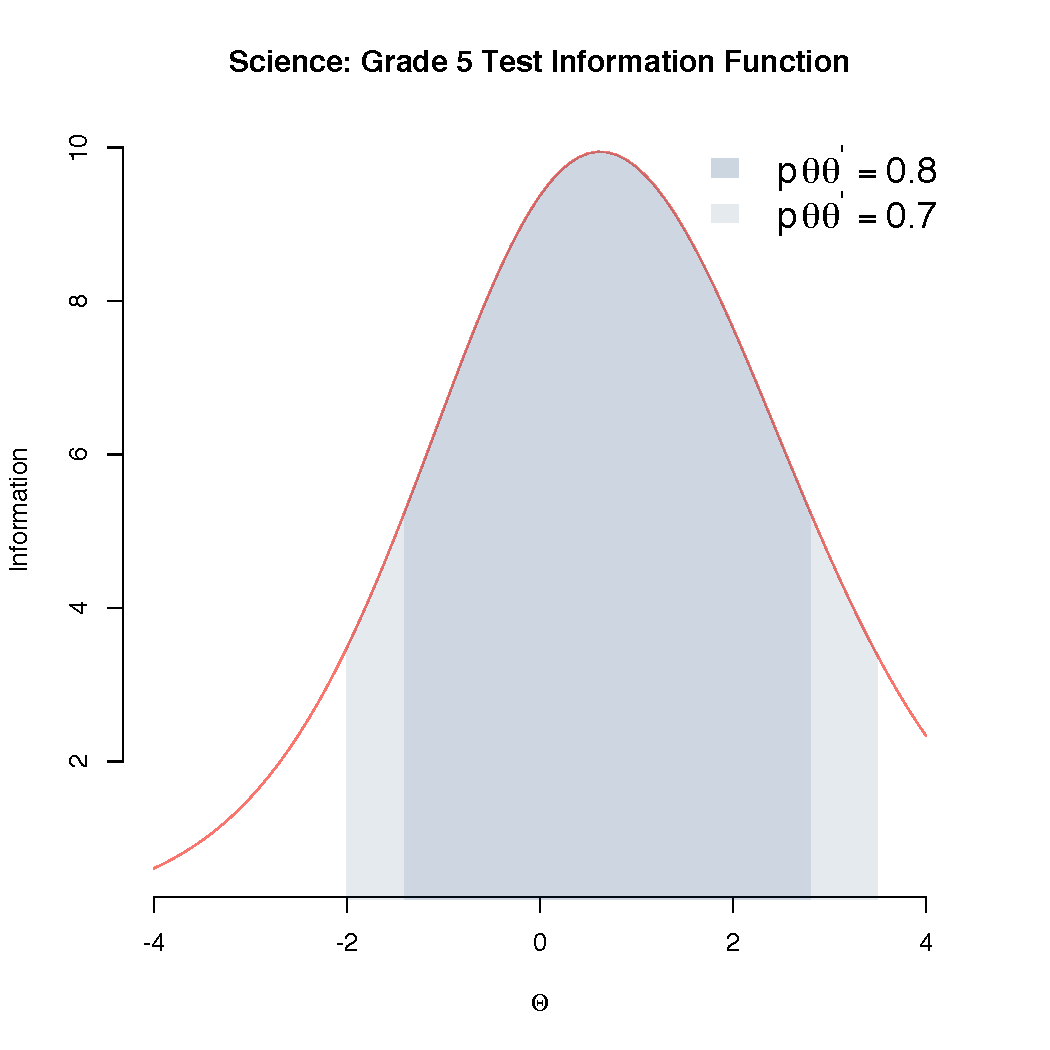
\includegraphics[height=3.12500in]{tifs/science5tif.pdf}
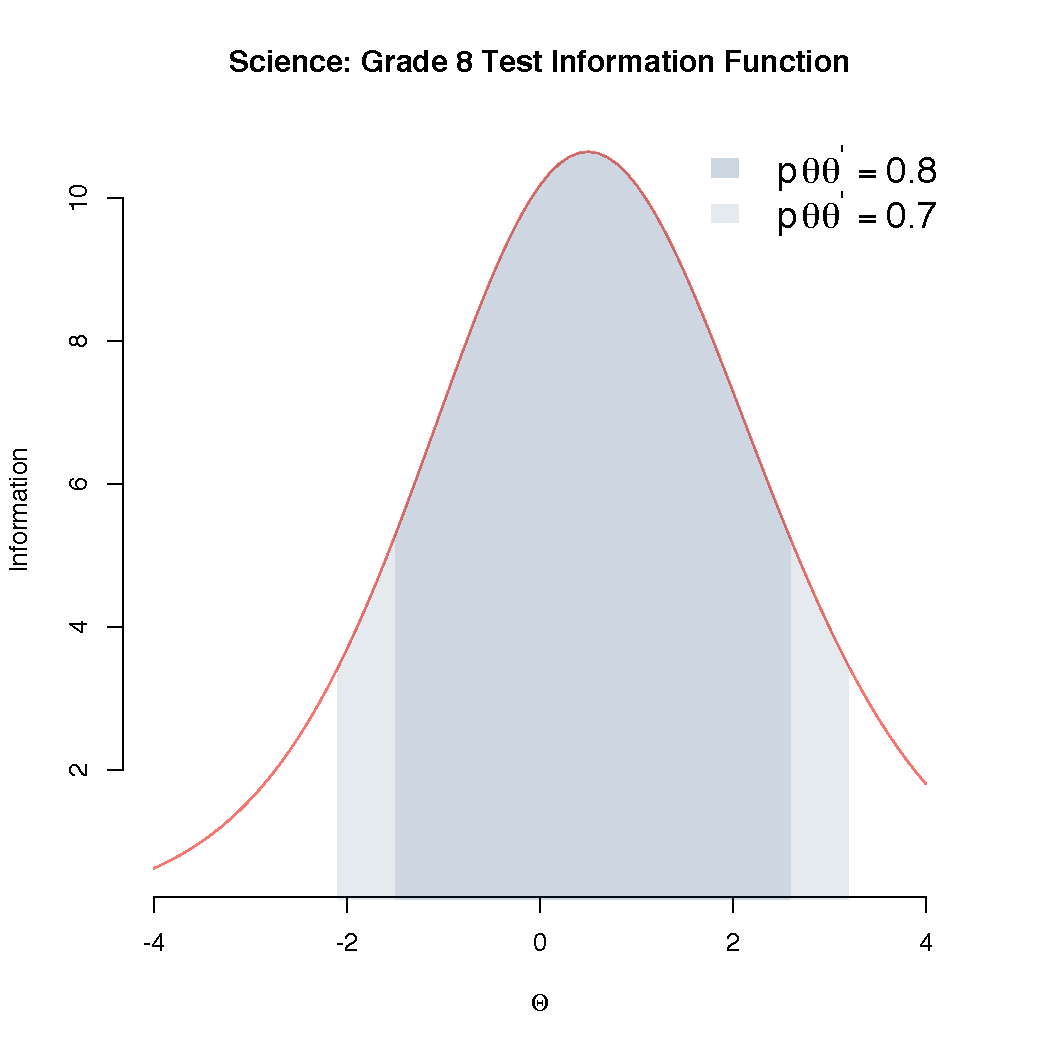
\includegraphics[height=3.12500in]{tifs/science8tif.pdf}
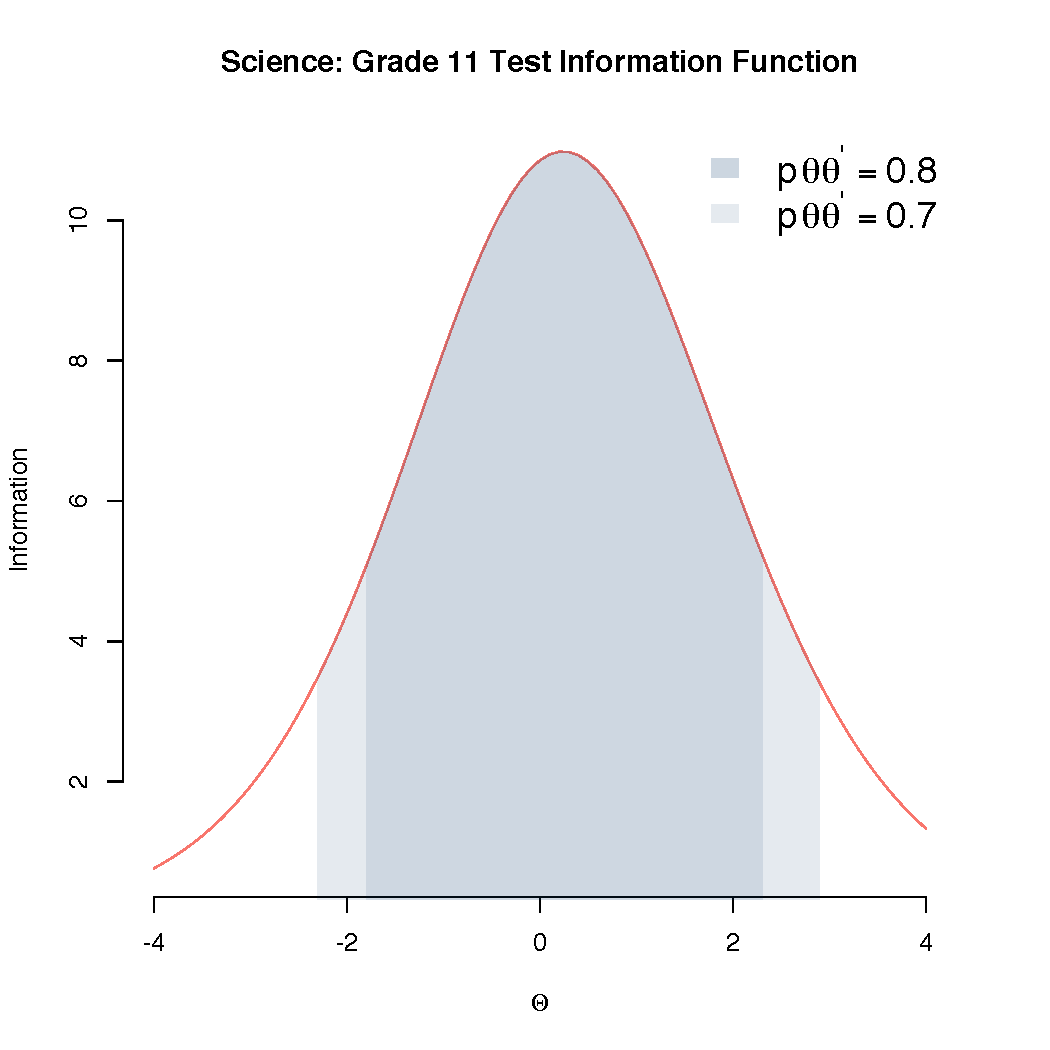
\includegraphics[height=3.12500in]{tifs/science11tif.pdf}

\subsubsection{Validation of ORExt Vertical
Scales}\label{validation-of-orext-vertical-scales}

The test characteristic curves (TCCs) for the grade-level assessments in
ELA and mathematics demonstrate incrementally increasing growth and test
demands across Grades 3-8, with the exception of Grade 7 mathematics.
The Grade 7 mathematics assessment was revised to be more difficult last
year, but clearly more elaboration of this effort is needed to address
its location on the TCC. Grade 11 and science tests are not vertically
scaled; TCCs are thus not presented for Grade 11 or science. All Rasch
model scaling, as well as the data visualizations for the TCCs were
conducted in the R software 3.3.2 environment (R Core Team, 2016) using
the r2Winsteps package (Anderson, 2015). \FloatBarrier
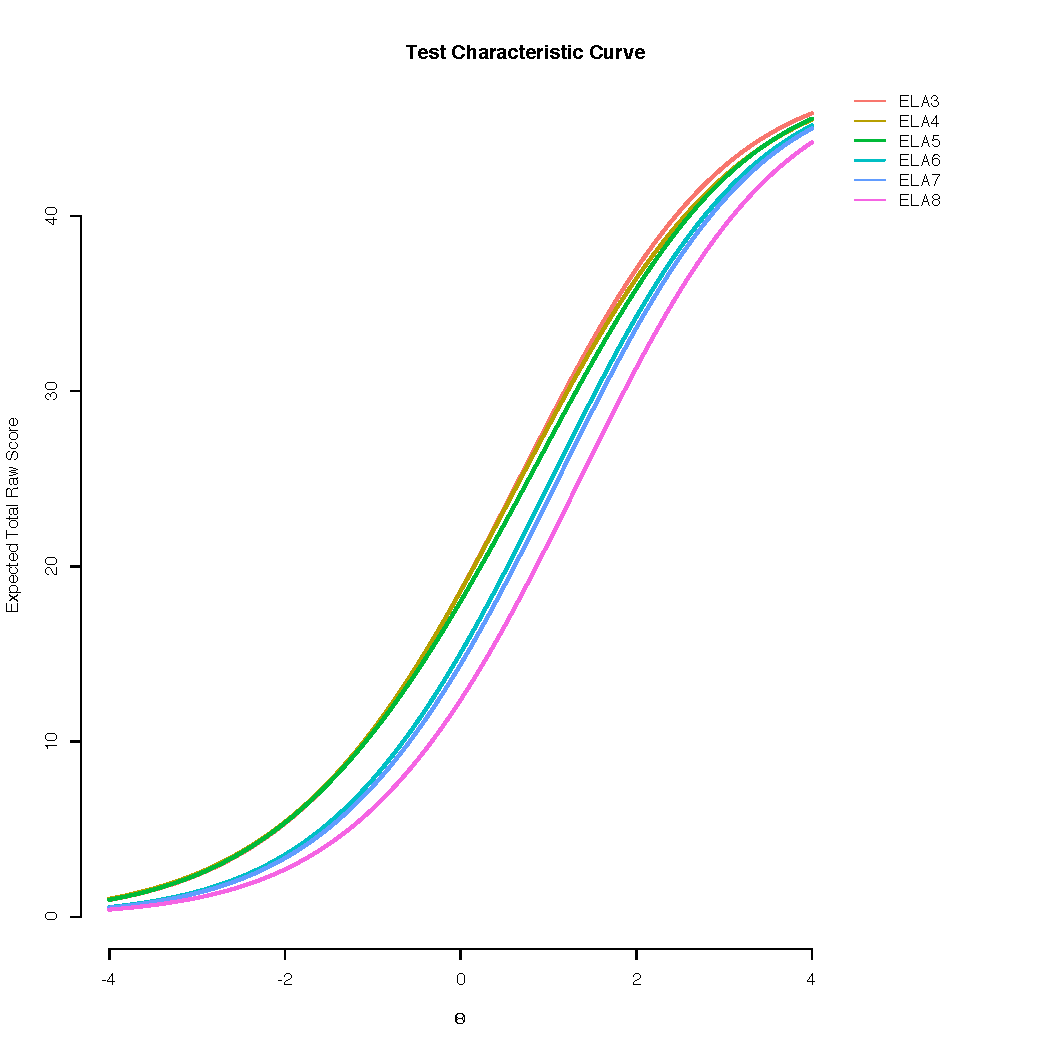
\includegraphics{tccs/ela_tccs.pdf} 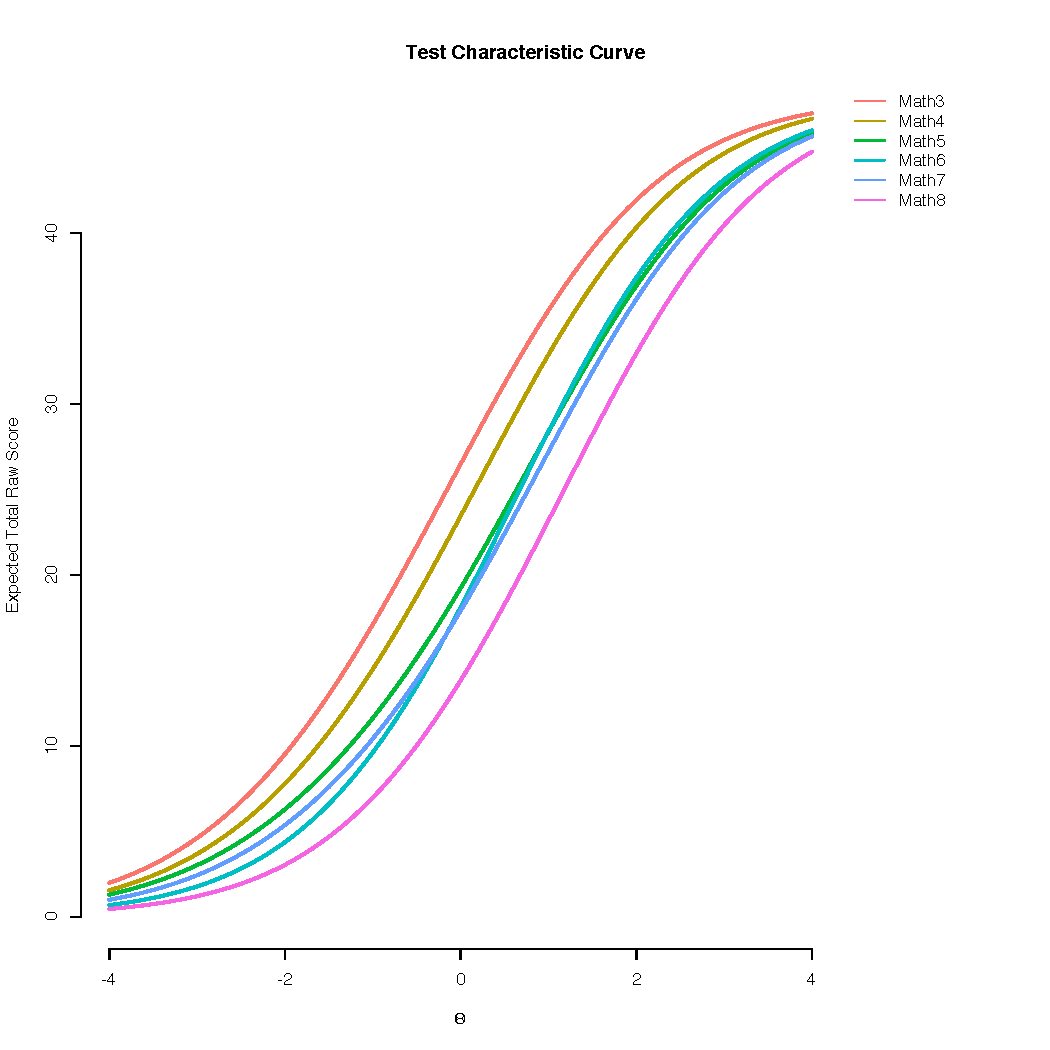
\includegraphics{tccs/math_tccs.pdf}
\clearpage

\paragraph{4.1B Overall and Conditional Standard Errors of
Measure}\label{b-overall-and-conditional-standard-errors-of-measure}

The average SEM associated with each cut score for 2017-18 student data
are presented in the table below, supported by a KEY. The SEMs decreased
in almost all cases compared to last year, suggesting that the measures
are more reliable when student eligibility is more strictly controlled.
See Section 4.2 below for means and standard deviations by grade and
subject area. SEM = Standard Error of Measure associated with the cut
score to the left; averaged to the tenths' place. Level 1 = Does Not Yet
Meet (not included as the lowest level of proficiency) Level 2 = Nearly
Meets Level 3 = Meets Level 4 = Exceeds

\FloatBarrier

\begin{table}[!h]

\caption{\label{tab:cut_score_se}ELA Cut Score Standard Errors}
\centering
\begin{tabu} to \linewidth {>{\raggedleft}X>{\raggedleft}X>{\raggedleft}X>{\raggedleft}X}
\toprule
Grade & AMO & RIT & SE\\
\midrule
3 & 2 & 192 & 4.41\\
3 & 3 & 213 & 3.83\\
3 & 4 & 228 & 5.06\\
4 & 2 & 201 & 3.86\\
4 & 3 & 214 & 3.95\\
\addlinespace
4 & 4 & 230 & 5.63\\
5 & 2 & 202 & 3.93\\
5 & 3 & 220 & 4.18\\
5 & 4 & 232 & 5.51\\
6 & 2 & 206 & 3.68\\
\addlinespace
6 & 3 & 220 & 3.84\\
6 & 4 & 234 & 5.45\\
7 & 2 & 208 & 3.66\\
7 & 3 & 222 & 4.08\\
7 & 4 & 236 & 6.17\\
\addlinespace
8 & 2 & 213 & 3.66\\
8 & 3 & 224 & 4.11\\
8 & 4 & 239 & 6.23\\
11 & 2 & 899 & 3.76\\
11 & 3 & 920 & 4.22\\
\addlinespace
11 & 4 & 927 & 5.01\\
12 & 2 & 906 & 3.60\\
12 & 3 & 924 & 4.67\\
12 & 4 & 929 & 5.48\\
\bottomrule
\end{tabu}
\end{table}\begin{table}[!h]

\caption{\label{tab:cut_score_se}Math Cut Score Standard Errors}
\centering
\begin{tabu} to \linewidth {>{\raggedleft}X>{\raggedleft}X>{\raggedleft}X>{\raggedleft}X}
\toprule
Grade & AMO & RIT & SE\\
\midrule
3 & 2 & 193 & 3.81\\
3 & 3 & 201 & 3.75\\
3 & 4 & 219 & 5.03\\
4 & 2 & 193 & 3.89\\
4 & 3 & 206 & 3.75\\
\addlinespace
4 & 4 & 219 & 4.69\\
5 & 2 & 193 & 4.28\\
5 & 3 & 207 & 3.76\\
5 & 4 & 220 & 4.28\\
6 & 2 & 205 & 3.64\\
\addlinespace
6 & 3 & 208 & 3.65\\
6 & 4 & 222 & 4.45\\
7 & 2 & 207 & 3.75\\
7 & 3 & 209 & 3.73\\
7 & 4 & 223 & 4.44\\
\addlinespace
8 & 2 & 208 & 3.67\\
8 & 3 & 212 & 3.61\\
8 & 4 & 226 & 4.22\\
11 & 2 & 901 & 3.59\\
11 & 3 & 908 & 3.59\\
\addlinespace
11 & 4 & 922 & 4.61\\
12 & 2 & 901 & 3.59\\
12 & 3 & 909 & 3.62\\
12 & 4 & 924 & 4.95\\
\bottomrule
\end{tabu}
\end{table}\begin{table}[!h]

\caption{\label{tab:cut_score_se}Science Cut Score Standard Errors}
\centering
\begin{tabu} to \linewidth {>{\raggedleft}X>{\raggedleft}X>{\raggedleft}X>{\raggedleft}X}
\toprule
Grade & AMO & RIT & SE\\
\midrule
5 & 2 & 506 & 3.73\\
5 & 3 & 517 & 3.80\\
5 & 4 & 531 & 5.11\\
8 & 2 & 810 & 3.57\\
8 & 3 & 820 & 4.05\\
\addlinespace
8 & 4 & 834 & 6.18\\
11 & 2 & 901 & 3.54\\
11 & 3 & 914 & 3.91\\
11 & 4 & 930 & 6.16\\
\bottomrule
\end{tabu}
\end{table}

\FloatBarrier

\paragraph{4.1C Classification Accuracy \&
Consistency}\label{c-classification-accuracy-consistency}

Results from the 2017-18 ORExt test administration were analyzed using
Rudner's classification index (Rudner, 2005). Results closer to 1.0
indicate the likelihood that a student was appropriately classified as
proficient or not proficient (accuracy) and the likelihood that the
student would be classified in the same category given an additional
test administration. The calculation utilizes item difficulty and theta
value distributions, as well as related standard errors of measurement,
to generate probabilistic estimates based on one test administration.
Complete results, generated from the cacIRT package in R, are provided
below. Results denote very high levels of classification accuracy and
consistency.

\FloatBarrier

\begin{table}[!h]

\caption{\label{tab:class_acc}ELA Accuracy/Consistency}
\centering
\begin{tabu} to \linewidth {>{\raggedleft}X>{\raggedleft}X>{\raggedleft}X>{\raggedleft}X}
\toprule
Grade & AMO & Accuracy & Consistency\\
\midrule
11 & 2 & 0.97 & 0.96\\
11 & 3 & 0.94 & 0.91\\
11 & 4 & 0.91 & 0.87\\
3 & 2 & 0.97 & 0.95\\
3 & 3 & 0.93 & 0.90\\
\addlinespace
3 & 4 & 0.96 & 0.95\\
4 & 2 & 0.95 & 0.93\\
4 & 3 & 0.93 & 0.91\\
4 & 4 & 0.93 & 0.90\\
5 & 2 & 0.96 & 0.94\\
\addlinespace
5 & 3 & 0.93 & 0.90\\
5 & 4 & 0.93 & 0.91\\
6 & 2 & 0.94 & 0.92\\
6 & 3 & 0.94 & 0.91\\
6 & 4 & 0.93 & 0.90\\
\addlinespace
7 & 2 & 0.95 & 0.93\\
7 & 3 & 0.93 & 0.91\\
7 & 4 & 0.92 & 0.89\\
8 & 2 & 0.95 & 0.92\\
8 & 3 & 0.92 & 0.88\\
8 & 4 & 0.94 & 0.92\\
\bottomrule
\end{tabu}
\end{table}\begin{table}[!h]

\caption{\label{tab:class_acc}Math Accuracy/Consistency}
\centering
\begin{tabu} to \linewidth {>{\raggedleft}X>{\raggedleft}X>{\raggedleft}X>{\raggedleft}X}
\toprule
Grade & AMO & Accuracy & Consistency\\
\midrule
11 & 2 & 0.91 & 0.88\\
11 & 3 & 0.91 & 0.87\\
11 & 4 & 0.96 & 0.94\\
3 & 2 & 0.91 & 0.88\\
3 & 3 & 0.91 & 0.88\\
\addlinespace
3 & 4 & 0.97 & 0.96\\
4 & 2 & 0.92 & 0.89\\
4 & 3 & 0.90 & 0.86\\
4 & 4 & 0.97 & 0.96\\
5 & 2 & 0.94 & 0.92\\
\addlinespace
5 & 3 & 0.89 & 0.85\\
5 & 4 & 0.97 & 0.96\\
6 & 2 & 0.89 & 0.85\\
6 & 3 & 0.90 & 0.85\\
6 & 4 & 0.98 & 0.97\\
\addlinespace
7 & 2 & 0.88 & 0.84\\
7 & 3 & 0.89 & 0.85\\
7 & 4 & 0.98 & 0.97\\
8 & 2 & 0.88 & 0.84\\
8 & 3 & 0.89 & 0.85\\
8 & 4 & 0.98 & 0.97\\
\bottomrule
\end{tabu}
\end{table}\begin{table}[!h]

\caption{\label{tab:class_acc}Science Accuracy/Consistency}
\centering
\begin{tabu} to \linewidth {>{\raggedleft}X>{\raggedleft}X>{\raggedleft}X>{\raggedleft}X}
\toprule
Grade & AMO & Accuracy & Consistency\\
\midrule
11 & 2 & 0.97 & 0.95\\
11 & 3 & 0.95 & 0.92\\
11 & 4 & 0.90 & 0.86\\
5 & 2 & 0.94 & 0.92\\
5 & 3 & 0.93 & 0.90\\
\addlinespace
5 & 4 & 0.92 & 0.90\\
8 & 2 & 0.94 & 0.92\\
8 & 3 & 0.94 & 0.92\\
8 & 4 & 0.91 & 0.88\\
\bottomrule
\end{tabu}
\end{table}

\FloatBarrier
The ORExt is not a computer-adaptive instrument so estimate precision
documentation based upon that test design is not provided.

\subsubsection{4.2 Fairness and
Accessibility}\label{fairness-and-accessibility}

The state has taken steps to ensure fairness in the development of the
assessments, including an analysis of each test item by Oregon teachers
not only for linkage to standards, but also for access, sensitivity, and
bias (see \emph{Appendix} 3.1A). In addition, we reviewed test
functioning as relevant to race/ethnicity and disability subgroups. This
process increases the likelihood that students are receiving instruction
in areas reflected in the assessment, and also that the items are not
biased toward a particular demographic or sub-group.

\clearpage
\FloatBarrier

\subparagraph{Differential Item Functioning
Analyses}\label{differential-item-functioning-analyses}

To investigate Differential Item Functioning (DIF), the Mantel-Haenszel
test using a purification process was conducted (Holland \& Thayer,
1988; Kamata \& Vaughn, 2004) with the R software using the difR package
(Magis et al., 2013). When using the Mantel-Haenszel test to investigate
DIF, contingency tables are constructed, and the resulting odds for the
focal group answering the item correctly are compared to the odds for
the reference group. Given n-size limitations (Scott, et al., 2009), we
were able to conduct two analyses: a) White/Non-White and b)
Male/Female. Whites and Males were the focal groups and Non-Whites and
Females were the reference groups, respectively. The contingency table
summarizes correct and incorrect responses to each item by respondents'
total raw score by subgroup (Kamata \& Vaughn, 2004). If there is no
difference in performance for the two groups, the odds ratio of the
focal group performance to reference group performance will equal one.
An odds ratio greater than one means the focal group is performing
better than the reference group, with the opposite being true for odds
ratios less than one.

The difR package contains a built in algorithm to conduct purification
automatically, so we were interested in how this algorithm functioned
relative to the iterations conducted manually using SPSS. We used
criteria outlined by the Educational Testing Service (ETS) for DIF
Classification (Holland \& Thayer, 1988) to determine whether or not
items exhibited DIF, as the difR package reports delta values by
default, defined as \[\Delta_{MH} =
-2.35*ln(\alpha_{MH})\]

The Holland and Thayer criteria were used for all Mantel-Haenszel
analyses. Items that were flagged as ``C'' level items were reviewed by
BRT researchers for potential biases. If biases are identified, the item
is removed from the item pool. DIF analyses were performed ex post facto
on the 2015-16 ORExt operational items to address longitudinal trends.
Only three ELA items were identified as exhibiting a ``C'' level DIF
across both 2017 and 2018. Those three ELA items, one in Grade 5 that
exhibited DIF that privileged White examinees, one in Grade 4 that
privileged Female examinees, and one in Grade 8 that privileged Female
examinees, were removed and were not used in 2017-18 or thereafter. DIF
analyses was also be performed in the 2017-18 school year to continue to
address DIF longitudinally. All items, including field test items, were
included in the analyses. There are a total of 48 items on each
assessment.

Within the White/Non-White analysis, 10 out of 18 items flagged as ``C''
level items privileged Non-White test participants in ELA, 2 out of 5
privileged Non-White test participants in Mathematics, and 2 out of 7
privileged Non-White test participants in Science. Overall, DIF flagging
bases on race was relatively balanced, with 14 privileging students who
were Non-White and 16 privileging students who were White.

\FloatBarrier

\begin{table}[!h]

\caption{\label{tab:dif1}ELA Differential Item Functioning Grades: White/Non-White}
\centering
\begin{tabu} to \linewidth {>{\raggedleft}X>{\raggedleft}X>{\raggedleft}X>{\raggedleft}X}
\toprule
Grade & A & B & C\\
\midrule
3 & 43 & 4 & 1\\
4 & 44 & 1 & 3\\
5 & 38 & 10 & 0\\
6 & 42 & 4 & 2\\
7 & 39 & 7 & 2\\
\addlinespace
8 & 35 & 10 & 3\\
11 & 36 & 9 & 3\\
\bottomrule
\end{tabu}
\end{table}\begin{table}[!h]

\caption{\label{tab:dif1}Math Differential Item Functioning Grades: White/Non-White}
\centering
\begin{tabu} to \linewidth {>{\raggedleft}X>{\raggedleft}X>{\raggedleft}X>{\raggedleft}X}
\toprule
Grade & A & B & C\\
\midrule
3 & 45 & 3 & 0\\
4 & 44 & 4 & 0\\
5 & 44 & 3 & 1\\
6 & 42 & 6 & 0\\
7 & 45 & 3 & 0\\
\addlinespace
8 & 45 & 2 & 1\\
11 & 42 & 6 & 0\\
\bottomrule
\end{tabu}
\end{table}\begin{table}[!h]

\caption{\label{tab:dif1}Science Differential Item Functioning Grades: White/Non-White}
\centering
\begin{tabu} to \linewidth {>{\raggedleft}X>{\raggedleft}X>{\raggedleft}X>{\raggedleft}X}
\toprule
Grade & A & B & C\\
\midrule
5 & 39 & 6 & 3\\
8 & 46 & 2 & 0\\
11 & 38 & 6 & 4\\
\bottomrule
\end{tabu}
\end{table}

\FloatBarrier

In terms of the Male/Female analyses, 10 out of 16 items flagged as
``C'' level items privileged Females in ELA, 4 out of 9 flagged items
privileged Females in Mathematics, and 8 out of 11 flagged items
privileged Females in Science. Overall, DIF flagging based on sex was
relatively balanced, with 22 privileging Females and 14 privileging
Males.

\begin{table}[!h]

\caption{\label{tab:gndr_dif}ELA Differential Item Functioning Grades: Male/Female}
\centering
\begin{tabu} to \linewidth {>{\raggedleft}X>{\raggedleft}X>{\raggedleft}X>{\raggedleft}X}
\toprule
Grade & A & B & C\\
\midrule
3 & 41 & 5 & 2\\
4 & 40 & 5 & 3\\
5 & 42 & 4 & 2\\
6 & 40 & 5 & 3\\
7 & 41 & 5 & 2\\
\addlinespace
8 & 40 & 5 & 3\\
11 & 34 & 6 & 8\\
\bottomrule
\end{tabu}
\end{table}\begin{table}[!h]

\caption{\label{tab:gndr_dif}Math Differential Item Functioning Grades: Male/Female}
\centering
\begin{tabu} to \linewidth {>{\raggedleft}X>{\raggedleft}X>{\raggedleft}X>{\raggedleft}X}
\toprule
Grade & A & B & C\\
\midrule
3 & 39 & 9 & 0\\
4 & 42 & 5 & 1\\
5 & 34 & 9 & 5\\
6 & 43 & 4 & 1\\
7 & 39 & 6 & 3\\
\addlinespace
8 & 43 & 5 & 0\\
11 & 43 & 5 & 0\\
\bottomrule
\end{tabu}
\end{table}\begin{table}[!h]

\caption{\label{tab:gndr_dif}Science Differential Item Functioning Grades: Male/Female}
\centering
\begin{tabu} to \linewidth {>{\raggedleft}X>{\raggedleft}X>{\raggedleft}X>{\raggedleft}X}
\toprule
Grade & A & B & C\\
\midrule
5 & 40 & 4 & 4\\
8 & 36 & 8 & 4\\
11 & 31 & 15 & 2\\
\bottomrule
\end{tabu}
\end{table}

\clearpage

\paragraph{Race - Ethnicity Percentages and Totals by Content Area and
Grade
Level}\label{race---ethnicity-percentages-and-totals-by-content-area-and-grade-level}

The full ethnic and disability demographics for students taking the
ORExt are reported below. Students ethnicity/race was reported in seven
categories: (a) American Indian/Alaskan Native, (b) Asian, (c) Black or
African-American, (d) Multi-ethnic, (e) Native Hawaiian or Other Pacific
Islander, (f) Hispanic, or (g) White. The majority of students were
reported as White (53-68\%) or Hispanic (12-27\%). These results are
largely consistent with the demographics reported for the general
assessments, though percentages taking the ORExt are slightly higher for
most students of color and generally lower for students who are Asian or
White (see \emph{Appendix} 4.2).

\begin{table}[!h]

\caption{\label{tab:eth_perc}Race/Ethnicity Proportions}
\centering
\begin{tabu} to \linewidth {>{\raggedright}X>{\raggedright}X>{\raggedleft}X>{\raggedleft}X>{\raggedleft}X>{\raggedleft}X>{\raggedleft}X>{\raggedleft}X>{\raggedleft}X}
\toprule
Grade & Content & Asian & Black & Hispanic & Am Ind & Multiethnic & Pac Isl & White\\
\midrule
03 & ELA & 3.33 & 4.26 & 27.04 & 1.67 & 9.26 & 1.11 & 53.33\\
03 & Math & 3.36 & 4.10 & 27.43 & 1.49 & 8.77 & 1.12 & 53.73\\
04 & ELA & 2.91 & 3.59 & 26.67 & 2.39 & 6.67 & 1.88 & 55.90\\
04 & Math & 2.90 & 3.58 & 27.13 & 2.39 & 6.66 & 1.88 & 55.46\\
05 & ELA & 4.74 & 3.23 & 27.32 & 1.90 & 6.64 & 1.14 & 55.03\\
\addlinespace
05 & Math & 4.92 & 3.22 & 27.46 & 1.70 & 6.44 & 1.14 & 55.11\\
05 & Science & 4.97 & 3.25 & 27.53 & 1.72 & 6.50 & 0.96 & 55.07\\
06 & ELA & 3.25 & 3.97 & 25.45 & 1.62 & 5.78 & 0.72 & 59.21\\
06 & Math & 3.43 & 3.97 & 25.09 & 1.62 & 5.78 & 0.72 & 59.39\\
07 & ELA & 3.86 & 2.85 & 26.42 & 2.85 & 8.74 & 0.81 & 54.47\\
\addlinespace
07 & Math & 3.91 & 2.67 & 26.95 & 2.67 & 8.44 & 0.82 & 54.53\\
08 & ELA & 4.41 & 4.41 & 23.95 & 2.52 & 6.09 & 1.26 & 57.35\\
08 & Math & 4.38 & 4.38 & 23.80 & 2.30 & 6.05 & 1.25 & 57.83\\
08 & Science & 4.22 & 4.43 & 23.21 & 2.32 & 6.12 & 1.27 & 58.44\\
11 & ELA & 4.43 & 4.43 & 22.14 & 2.33 & 3.73 & 0.70 & 62.24\\
\addlinespace
11 & Math & 4.40 & 4.40 & 22.22 & 2.31 & 3.70 & 0.69 & 62.27\\
11 & Science & 4.27 & 4.03 & 22.04 & 2.13 & 3.79 & 0.71 & 63.03\\
12 & ELA & 0.00 & 16.67 & 20.83 & 4.17 & 4.17 & 0.00 & 54.17\\
12 & Math & 0.00 & 10.71 & 25.00 & 3.57 & 3.57 & 0.00 & 57.14\\
12 & Science & 0.00 & 12.50 & 12.50 & 6.25 & 0.00 & 0.00 & 68.75\\
\bottomrule
\end{tabu}
\end{table}

Student reported exceptionalities included Intellectual Disability (ID
10), Hearing Impairment (HI 20), Visual Impairment (VI 40),
Deaf-Blindness (DB 43), Communication Disorder (CD 50), Emotional
Disturbance (ED 60), Orthopedic Impairment (OI 70), Traumatic Brain
Injury (TBI 74), Other Health Impairment (OHI 80), Autism Spectrum
Disorder (ASD 82), and Specific Learning Disability (SLD 90). The
majority of students who participated in the ORExt were students with ID
(30-45\%) and students with ASD (28 -34\%), followed by students with
OHI (11 -16\%). ODE policy for 2015-16 changed to require students who
participate in the ORExt to take the assessment in all relevant content
areas. There is thus very little change in terms of participation
percentages across content areas, as evidenced by the total n-sizes per
grade level displayed below.

\clearpage

\paragraph{Exceptionality Percentages By Content Area and Grade
Level}\label{exceptionality-percentages-by-content-area-and-grade-level}

\begin{table}[!h]

\caption{\label{tab:disab_perc}Disability Proportions}
\centering
\begin{tabu} to \linewidth {>{\raggedleft}X>{\raggedright}X>{\raggedleft}X>{\raggedleft}X>{\raggedleft}X>{\raggedleft}X>{\raggedleft}X>{\raggedleft}X>{\raggedleft}X>{\raggedleft}X>{\raggedleft}X>{\raggedleft}X>{\raggedleft}X>{\raggedleft}X}
\toprule
Grade & Content & 0 & 10 & 20 & 40 & 43 & 50 & 60 & 70 & 74 & 80 & 82 & 90\\
\midrule
3 & ela & 2.59 & 27.96 & 0.74 & 1.11 & 0.00 & 6.67 & 1.85 & 4.81 & 0.74 & 14.81 & 35.93 & 2.78\\
3 & math & 2.24 & 27.99 & 0.93 & 1.12 & 0.00 & 6.72 & 1.87 & 4.85 & 0.93 & 15.11 & 35.45 & 2.80\\
4 & ela & 3.42 & 37.44 & 0.34 & 0.17 & 0.00 & 4.96 & 1.71 & 3.25 & 0.68 & 12.65 & 30.26 & 5.13\\
4 & math & 2.90 & 37.37 & 0.34 & 0.17 & 0.00 & 5.46 & 1.71 & 3.07 & 0.68 & 12.63 & 30.55 & 5.12\\
5 & ela & 3.23 & 38.14 & 0.00 & 0.19 & 0.00 & 5.50 & 1.90 & 3.98 & 1.71 & 11.01 & 29.60 & 4.74\\
\addlinespace
5 & math & 3.22 & 38.45 & 0.00 & 0.19 & 0.00 & 5.49 & 1.89 & 3.79 & 1.52 & 11.36 & 29.36 & 4.73\\
5 & sci & 3.06 & 38.81 & 0.00 & 0.19 & 0.00 & 5.54 & 1.91 & 3.82 & 1.72 & 11.47 & 28.68 & 4.78\\
6 & ela & 2.53 & 43.86 & 0.54 & 0.18 & 0.00 & 3.97 & 1.08 & 1.81 & 0.90 & 12.82 & 28.88 & 3.43\\
6 & math & 2.71 & 44.22 & 0.54 & 0.18 & 0.00 & 3.97 & 0.90 & 1.81 & 0.72 & 12.45 & 29.06 & 3.43\\
7 & ela & 2.03 & 39.63 & 0.20 & 1.02 & 0.00 & 3.66 & 1.42 & 2.64 & 0.61 & 11.38 & 34.76 & 2.64\\
\addlinespace
7 & math & 2.06 & 39.92 & 0.21 & 1.03 & 0.00 & 3.70 & 1.23 & 2.88 & 0.62 & 11.11 & 34.77 & 2.47\\
8 & ela & 2.10 & 39.92 & 0.42 & 0.21 & 0.00 & 2.10 & 2.10 & 4.20 & 0.84 & 14.08 & 30.46 & 3.57\\
8 & math & 2.51 & 40.08 & 0.42 & 0.21 & 0.00 & 2.09 & 2.09 & 4.18 & 0.84 & 13.57 & 30.48 & 3.55\\
8 & sci & 2.74 & 39.66 & 0.42 & 0.21 & 0.00 & 2.11 & 2.32 & 4.01 & 0.84 & 13.50 & 30.59 & 3.59\\
11 & ela & 6.99 & 47.09 & 0.47 & 1.17 & 0.23 & 2.33 & 1.63 & 2.10 & 0.00 & 10.26 & 23.31 & 4.43\\
\addlinespace
11 & math & 6.94 & 47.22 & 0.46 & 1.16 & 0.23 & 2.31 & 1.62 & 2.31 & 0.00 & 10.42 & 23.15 & 4.17\\
11 & sci & 7.11 & 46.92 & 0.47 & 1.18 & 0.24 & 2.37 & 1.66 & 2.13 & 0.24 & 10.66 & 22.75 & 4.27\\
12 & ela & 8.33 & 54.17 & 0.00 & 0.00 & 0.00 & 0.00 & 4.17 & 0.00 & 0.00 & 4.17 & 25.00 & 4.17\\
12 & math & 14.29 & 50.00 & 0.00 & 0.00 & 0.00 & 0.00 & 3.57 & 0.00 & 0.00 & 3.57 & 25.00 & 3.57\\
\bottomrule
\end{tabu}
\end{table}

\paragraph{Observed Means and Standard
Deviations}\label{observed-means-and-standard-deviations}

The following tables provide information regarding observed means and
standard deviations by content area and grade level. The Grade 3-8
English language arts and mathematics scaled scores are centered on 200,
while all Grade 11 scores are centered on 900 (to reinforce that they
are not on the vertical scale). Science is centered on 500 at Grade 5
and centered on 800 at Grade 8. The vertically scaled scores generally
convey incremental gains in achievement across grade levels, though the
results suggest small losses across grades in math.These scales were
selected to clearly determine whether scores are on the same scale and
also to differentiate among the statewide assessments in use to avoid
confusion (i.e., SBA, OAKS, ORExt, ELPA, KA). The general pattern is
that RIT scores decreased from 2014-15 to 2015-16. This decrease is
attributed not to the scale, nor to deceleration of growth, but to the
substantive shift in the tested student population as a result of ODE
eligibility guidelines. The scale from 2015-16 to 2016-17 appears to
have stabilized because the student population tested was more
consistent.

\begin{table}[!h]

\caption{\label{tab:unnamed-chunk-3}Means/SDs: 2014-15}
\centering
\begin{tabu} to \linewidth {>{\raggedleft}X>{\raggedleft}X>{\raggedleft}X>{\raggedleft}X>{\raggedleft}X>{\raggedleft}X>{\raggedleft}X}
\toprule
Grade & ELA.Mean & ELA.SD & Math.Mean & Math.SD & Sci.Mean & Sci.SD\\
\midrule
3 & 219.3 & 24.6 & 201.5 & 20.8 &  & \\
4 & 222.8 & 23.6 & 204.8 & 19.8 &  & \\
5 & 224.9 & 25.0 & 205.3 & 18.1 & 517.6 & 25.6\\
6 & 226.3 & 24.0 & 207.7 & 17.7 &  & \\
7 & 226.4 & 25.0 & 207.9 & 19.0 &  & \\
\addlinespace
8 & 225.4 & 24.1 & 207.8 & 17.3 & 822.1 & 25.8\\
11 & 922.5 & 28.5 & 903.8 & 21.1 & 920.8 & 27.7\\
\bottomrule
\end{tabu}
\end{table}

\begin{table}[!h]

\caption{\label{tab:unnamed-chunk-3}Means/SDs: 2015-16}
\centering
\begin{tabu} to \linewidth {>{\raggedleft}X>{\raggedleft}X>{\raggedleft}X>{\raggedleft}X>{\raggedleft}X>{\raggedleft}X>{\raggedleft}X}
\toprule
Grade & ElA.Mean & ELA.SD & Math.Mean & Math.SD & Science.Mean & Science.SD\\
\midrule
3 & 210.3 & 23.0 & 197.6 & 20.2 &  & \\
4 & 212.3 & 22.9 & 198.1 & 18.7 &  & \\
5 & 217.1 & 24.5 & 201.2 & 17.2 & 514.2 & 22.1\\
6 & 220.1 & 25.5 & 204.8 & 17.6 &  & \\
7 & 223.6 & 28.9 & 205.4 & 19.0 &  & \\
\addlinespace
8 & 221.2 & 24.8 & 206.7 & 17.2 & 819.0 & 25.6\\
11 & 920.7 & 27.7 & 902.3 & 20.0 & 918.0 & 24.9\\
\bottomrule
\end{tabu}
\end{table}

\begin{table}[!h]

\caption{\label{tab:unnamed-chunk-3}Means/SDs: 2016-17}
\centering
\begin{tabu} to \linewidth {>{\raggedleft}X>{\raggedleft}X>{\raggedleft}X>{\raggedleft}X>{\raggedleft}X>{\raggedleft}X>{\raggedleft}X}
\toprule
Grade & ElA.Mean & ELA.SD & Math.Mean & Math.SD & Science.Mean & Science.SD\\
\midrule
3 & 210.3 & 23.0 & 197.6 & 20.2 &  & \\
4 & 212.3 & 22.9 & 198.1 & 18.7 &  & \\
5 & 217.1 & 24.5 & 201.2 & 17.2 & 514.2 & 22.1\\
6 & 220.1 & 25.5 & 204.8 & 17.6 &  & \\
7 & 223.6 & 28.9 & 205.4 & 19.0 &  & \\
\addlinespace
8 & 221.2 & 24.8 & 206.7 & 17.2 & 819.0 & 25.6\\
11 & 920.7 & 27.7 & 902.3 & 20.0 & 918.0 & 24.9\\
\bottomrule
\end{tabu}
\end{table}

\begin{table}[!h]

\caption{\label{tab:obs_means}Means/SDs: 2017-18}
\centering
\begin{tabu} to \linewidth {>{\raggedleft}X>{\raggedleft}X>{\raggedleft}X>{\raggedleft}X>{\raggedleft}X>{\raggedleft}X>{\raggedleft}X}
\toprule
Grade & ELA Mean & ELA SD & Math Mean & Math SD & Sci Mean & Sci SD\\
\midrule
3 & 204.61 & 21.60 & 192.19 & 19.66 &  & \\
4 & 212.25 & 22.99 & 197.83 & 16.82 &  & \\
5 & 213.08 & 25.52 & 198.92 & 17.06 & 512.38 & 21.03\\
6 & 213.07 & 23.61 & 199.77 & 16.71 &  & \\
7 & 215.07 & 23.49 & 201.24 & 17.18 &  & \\
\addlinespace
8 & 216.69 & 23.03 & 204.25 & 16.28 & 816.65 & 23.06\\
11 & 917.99 & 26.94 & 901.80 & 17.89 & 917.42 & 24.79\\
12 & 934.21 & 22.65 & 904.46 & 22.92 &  & \\
\bottomrule
\end{tabu}
\end{table}

\clearpage

\paragraph{Observed Means Reported by
Sex}\label{observed-means-reported-by-sex}

The following tables provide information regarding average student
performance by grade level and sex (Female/Male) in each of the content
areas assessed on the ORExt. Significant differences based on a Welch
two sample t-test are noted in Grades 5 and 12 in ELA, and Grade 8 in
mathematics.

\begin{table}[!h]

\caption{\label{tab:obs_means_sex}Means/SDs by Gender: 2017-18}
\centering
\begin{tabu} to \linewidth {>{\raggedleft}X>{\raggedright}X>{\raggedleft}X>{\raggedleft}X>{\raggedleft}X>{\raggedleft}X>{\raggedleft}X>{\raggedleft}X}
\toprule
Grade & Sex & ELA Mean & ELA SD & Math Mean & Math SD & Sci Mean & Sci SD\\
\midrule
3 & F & 203.72 & 22.21 & 190.77 & 19.47 &  & \\
3 & M & 205.01 & 21.34 & 192.82 & 19.74 &  & \\
4 & F & 212.62 & 22.62 & 197.57 & 17.64 &  & \\
4 & M & 212.09 & 23.17 & 197.94 & 16.47 &  & \\
5 & F & 209.74 & 25.74 & 197.11 & 17.64 & 508.85 & 21.81\\
\addlinespace
5 & M & 214.88 & 25.26 & 199.90 & 16.67 & 514.32 & 20.37\\
6 & F & 214.54 & 23.98 & 199.66 & 16.85 &  & \\
6 & M & 212.21 & 23.39 & 199.84 & 16.65 &  & \\
7 & F & 215.45 & 24.39 & 199.88 & 17.30 &  & \\
7 & M & 214.88 & 23.08 & 201.90 & 17.11 &  & \\
\addlinespace
8 & F & 216.50 & 25.01 & 201.98 & 17.73 & 813.97 & 23.89\\
8 & M & 216.78 & 22.09 & 205.30 & 15.48 & 817.88 & 22.59\\
11 & F & 917.73 & 27.21 & 900.46 & 15.90 & 916.00 & 24.15\\
11 & M & 918.14 & 26.83 & 902.55 & 18.90 & 918.24 & 25.15\\
12 & F & 943.80 & 12.08 & 902.92 & 23.84 &  & \\
12 & M & 927.36 & 26.18 & 905.80 & 22.85 &  & \\
\bottomrule
\end{tabu}
\end{table}

\clearpage

\paragraph{Observed Means Reported by
Race}\label{observed-means-reported-by-race}

The following table provides information regarding average student
performance by grade level and race/ethnicity in each of the content
areas assessed on the ORExt.

\begin{table}[!h]

\caption{\label{tab:eth_means}Grade 3 Means/SDs by Race/Ethnicity: 2017-18}
\centering
\begin{tabu} to \linewidth {>{\raggedright}X>{\raggedleft}X>{\raggedleft}X>{\raggedleft}X>{\raggedleft}X}
\toprule
Eth Code & ELA Mn & ELA SD & Math Mn & Math SD\\
\midrule
A & 200.83 & 21.53 & 188.56 & 21.90\\
B & 199.22 & 17.90 & 186.45 & 19.66\\
H & 202.36 & 20.08 & 191.30 & 18.40\\
I & 199.78 & 19.58 & 193.62 & 16.73\\
M & 203.24 & 22.36 & 191.34 & 22.24\\
\addlinespace
P & 204.33 & 22.40 & 194.00 & 18.26\\
W & 206.82 & 22.44 & 193.38 & 19.86\\
\bottomrule
\end{tabu}
\end{table}\begin{table}[!h]

\caption{\label{tab:eth_means}Grade 4 Means/SDs by Race/Ethnicity: 2017-18}
\centering
\begin{tabu} to \linewidth {>{\raggedright}X>{\raggedleft}X>{\raggedleft}X>{\raggedleft}X>{\raggedleft}X}
\toprule
Eth Code & ELA Mn & ELA SD & Math Mn & Math SD\\
\midrule
A & 204.88 & 18.09 & 191.47 & 17.18\\
B & 211.38 & 24.07 & 193.14 & 19.51\\
H & 209.62 & 21.79 & 196.18 & 17.34\\
I & 221.86 & 24.78 & 201.57 & 21.08\\
M & 216.62 & 20.99 & 198.33 & 15.00\\
\addlinespace
P & 222.55 & 18.72 & 205.45 & 10.84\\
W & 212.66 & 23.80 & 198.79 & 16.42\\
\bottomrule
\end{tabu}
\end{table}\begin{table}[!h]

\caption{\label{tab:eth_means}Grade 5 Means/SDs by Race/Ethnicity: 2017-18}
\centering
\begin{tabu} to \linewidth {>{\raggedright}X>{\raggedleft}X>{\raggedleft}X>{\raggedleft}X>{\raggedleft}X>{\raggedleft}X>{\raggedleft}X}
\toprule
Eth Code & ELA Mn & ELA SD & Math Mn & Math SD & Sci Mn & Sci SD\\
\midrule
A & 201.20 & 27.31 & 192.69 & 21.59 & 495.58 & 24.31\\
B & 209.82 & 27.63 & 192.94 & 20.15 & 508.88 & 22.74\\
H & 212.66 & 23.62 & 199.63 & 14.82 & 512.59 & 19.15\\
I & 214.40 & 38.49 & 200.44 & 20.98 & 517.33 & 23.32\\
M & 210.91 & 24.07 & 197.47 & 19.36 & 509.03 & 22.92\\
\addlinespace
P & 220.50 & 19.73 & 198.33 & 12.31 & 514.40 & 12.88\\
W & 214.57 & 25.83 & 199.60 & 17.11 & 514.20 & 20.78\\
\bottomrule
\end{tabu}
\end{table}\begin{table}[!h]

\caption{\label{tab:eth_means}Grade 6 Means/SDs by Race/Ethnicity: 2017-18}
\centering
\begin{tabu} to \linewidth {>{\raggedright}X>{\raggedleft}X>{\raggedleft}X>{\raggedleft}X>{\raggedleft}X}
\toprule
Eth Code & ELA Mn & ELA SD & Math Mn & Math SD\\
\midrule
A & 204.72 & 16.51 & 194.11 & 13.19\\
B & 210.95 & 25.17 & 196.36 & 18.27\\
H & 212.52 & 22.71 & 200.11 & 16.33\\
I & 200.00 & 22.24 & 194.00 & 17.79\\
M & 223.53 & 14.96 & 208.12 & 11.57\\
\addlinespace
P & 213.50 & 15.02 & 199.50 & 18.19\\
W & 213.24 & 24.75 & 199.53 & 17.14\\
\bottomrule
\end{tabu}
\end{table}\begin{table}[!h]

\caption{\label{tab:eth_means}Grade 7 Means/SDs by Race/Ethnicity: 2017-18}
\centering
\begin{tabu} to \linewidth {>{\raggedright}X>{\raggedleft}X>{\raggedleft}X>{\raggedleft}X>{\raggedleft}X}
\toprule
Eth Code & ELA Mn & ELA SD & Math Mn & Math SD\\
\midrule
A & 203.21 & 25.29 & 196.05 & 19.76\\
B & 201.86 & 24.21 & 189.62 & 24.91\\
H & 219.82 & 22.18 & 202.75 & 16.57\\
I & 209.57 & 24.44 & 207.38 & 6.08\\
M & 213.67 & 25.35 & 203.15 & 14.79\\
\addlinespace
P & 206.50 & 16.28 & 200.25 & 5.32\\
W & 214.94 & 23.23 & 200.86 & 17.46\\
\bottomrule
\end{tabu}
\end{table}\begin{table}[!h]

\caption{\label{tab:eth_means}Grade 8 Means/SDs by Race/Ethnicity: 2017-18}
\centering
\begin{tabu} to \linewidth {>{\raggedright}X>{\raggedleft}X>{\raggedleft}X>{\raggedleft}X>{\raggedleft}X>{\raggedleft}X>{\raggedleft}X}
\toprule
Eth Code & ELA Mn & ELA SD & Math Mn & Math SD & Sci Mn & Sci SD\\
\midrule
A & 209.76 & 16.92 & 203.52 & 12.55 & 815.40 & 17.17\\
B & 214.48 & 17.45 & 202.00 & 15.47 & 812.67 & 19.07\\
H & 212.32 & 24.42 & 201.13 & 20.00 & 811.76 & 25.55\\
I & 227.17 & 17.94 & 213.82 & 7.80 & 830.55 & 12.09\\
M & 219.10 & 21.99 & 204.52 & 18.29 & 819.07 & 19.73\\
\addlinespace
P & 222.83 & 12.77 & 211.83 & 2.99 & 818.00 & 13.16\\
W & 218.37 & 23.41 & 205.18 & 14.84 & 818.16 & 23.18\\
\bottomrule
\end{tabu}
\end{table}\begin{table}[!h]

\caption{\label{tab:eth_means}Grade 11 Means/SDs by Race/Ethnicity: 2017-18}
\centering
\begin{tabu} to \linewidth {>{\raggedright}X>{\raggedleft}X>{\raggedleft}X>{\raggedleft}X>{\raggedleft}X>{\raggedleft}X>{\raggedleft}X}
\toprule
Eth Code & ELA Mn & ELA SD & Math Mn & Math SD & Sci Mn & Sci SD\\
\midrule
A & 899.63 & 28.62 & 892.53 & 19.35 & 901.94 & 23.02\\
B & 913.63 & 33.91 & 899.53 & 22.03 & 911.29 & 31.30\\
H & 919.11 & 23.21 & 901.66 & 16.45 & 916.77 & 21.64\\
I & 925.70 & 21.86 & 902.60 & 12.97 & 919.00 & 10.90\\
M & 919.69 & 31.43 & 902.50 & 18.45 & 918.88 & 30.83\\
\addlinespace
P & 937.67 & 23.86 & 910.67 & 14.74 & 933.67 & 20.50\\
W & 918.60 & 27.10 & 902.50 & 18.08 & 918.77 & 25.22\\
\bottomrule
\end{tabu}
\end{table}\begin{table}[!h]

\caption{\label{tab:eth_means}Grade 12 Means/SDs by Race/Ethnicity: 2017-18}
\centering
\begin{tabu} to \linewidth {>{\raggedright}X>{\raggedleft}X>{\raggedleft}X>{\raggedleft}X>{\raggedleft}X}
\toprule
Eth Code & ELA Mn & ELA SD & Math Mn & Math SD\\
\midrule
B & 944.00 & 15.10 & 914.00 & 13.86\\
H & 935.20 & 14.64 & 903.43 & 23.33\\
I & 957.00 &  & 924.00 & \\
M & 906.00 &  & 901.00 & \\
W & 931.23 & 26.52 & 902.12 & 25.53\\
\bottomrule
\end{tabu}
\end{table}

\clearpage

\paragraph{Observed Means Reported by Exceptionality
Status}\label{observed-means-reported-by-exceptionality-status}

The following table is a number key for \textbf{Elibibility Codes:}

\subparagraph{Eligibility Codes List}\label{eligibility-codes-list}

\begin{itemize}
\tightlist
\item
  0 Not Applicable
\item
  10 Intellectual Disability
\item
  20 Hearing Impairment
\item
  40 Vision Impairment
\item
  43 Deafblindness
\item
  50 Communication Disorder
\item
  60 Emotional Disturbance
\item
  70 Orthopedic Impairment
\item
  74 Traumatic Brain Injury
\item
  80 Other Health Impairment
\item
  82 Autism Spectrum Disorder
\item
  90 Specific Learning Disability
\end{itemize}

The following tables provide information regarding average student
performance by grade level and exceptionality category in each of the
content areas assessed on the ORExt. Students with SLD were generally
the highest performing group, though students with ED performed higher
at certain grade levels/content areas. The lowest performing group was
consistently students with VI.

\begin{table}[!h]

\caption{\label{tab:disab_means}Grade 3 Means/SDs by Race/Ethnicity: 2017-18}
\centering
\begin{tabu} to \linewidth {>{\raggedleft}X>{\raggedleft}X>{\raggedleft}X>{\raggedleft}X>{\raggedleft}X}
\toprule
Dis Code & ELA Mean & ELA SD & Math Mean & Math SD\\
\midrule
0 & 199.57 & 24.29 & 193.08 & 19.88\\
10 & 204.09 & 16.96 & 191.61 & 16.45\\
20 & 214.75 & 16.58 & 198.80 & 13.77\\
40 & 175.67 & 28.30 & 165.00 & 26.00\\
50 & 212.67 & 17.71 & 200.86 & 14.83\\
\addlinespace
60 & 223.90 & 19.12 & 211.00 & 12.50\\
70 & 187.12 & 25.74 & 177.19 & 26.34\\
74 & 210.25 & 15.41 & 195.20 & 4.76\\
80 & 205.70 & 22.78 & 192.65 & 19.86\\
82 & 204.30 & 22.61 & 191.07 & 20.31\\
90 & 218.33 & 10.73 & 209.47 & 5.29\\
\bottomrule
\end{tabu}
\end{table}\begin{table}[!h]

\caption{\label{tab:disab_means}Grade 4 Means/SDs by Race/Ethnicity: 2017-18}
\centering
\begin{tabu} to \linewidth {>{\raggedleft}X>{\raggedleft}X>{\raggedleft}X>{\raggedleft}X>{\raggedleft}X}
\toprule
Dis Code & ELA Mean & ELA SD & Math Mean & Math SD\\
\midrule
0 & 189.50 & 30.87 & 190.65 & 19.95\\
10 & 213.70 & 19.18 & 198.59 & 14.86\\
20 & 220.00 & 36.77 & 203.00 & 25.46\\
40 & 148.00 &  & 145.00 & \\
50 & 221.31 & 11.08 & 203.94 & 9.57\\
\addlinespace
60 & 227.90 & 10.84 & 209.60 & 8.13\\
70 & 186.42 & 28.03 & 179.00 & 25.90\\
74 & 185.75 & 38.91 & 177.50 & 27.86\\
80 & 212.91 & 23.26 & 198.89 & 16.42\\
82 & 210.75 & 22.76 & 195.89 & 17.12\\
90 & 231.57 & 16.67 & 210.17 & 7.06\\
\bottomrule
\end{tabu}
\end{table}\begin{table}[!h]

\caption{\label{tab:disab_means}Grade 5 Means/SDs by Race/Ethnicity: 2017-18}
\centering
\begin{tabu} to \linewidth {>{\raggedleft}X>{\raggedleft}X>{\raggedleft}X>{\raggedleft}X>{\raggedleft}X>{\raggedleft}X>{\raggedleft}X}
\toprule
Dis Code & ELA Mean & ELA SD & Math Mean & Math SD & Sci Mean & Sci SD\\
\midrule
0 & 193.82 & 27.72 & 184.76 & 23.43 & 503.19 & 20.89\\
10 & 212.00 & 22.97 & 198.36 & 15.26 & 511.47 & 18.69\\
40 & 163.00 &  & 149.00 &  & 469.00 & \\
50 & 222.14 & 11.32 & 207.93 & 7.10 & 524.38 & 8.41\\
60 & 238.30 & 17.77 & 210.70 & 7.33 & 534.10 & 9.42\\
\addlinespace
70 & 174.38 & 30.12 & 171.45 & 24.32 & 482.35 & 26.94\\
74 & 224.33 & 20.13 & 205.38 & 16.33 & 525.11 & 12.23\\
80 & 218.78 & 22.88 & 202.70 & 13.19 & 516.22 & 18.29\\
82 & 212.69 & 25.38 & 198.86 & 16.39 & 509.37 & 21.76\\
90 & 233.96 & 13.11 & 211.08 & 6.95 & 533.00 & 6.93\\
\bottomrule
\end{tabu}
\end{table}\begin{table}[!h]

\caption{\label{tab:disab_means}Grade 6 Means/SDs by Race/Ethnicity: 2017-18}
\centering
\begin{tabu} to \linewidth {>{\raggedleft}X>{\raggedleft}X>{\raggedleft}X>{\raggedleft}X>{\raggedleft}X}
\toprule
Dis Code & ELA Mean & ELA SD & Math Mean & Math SD\\
\midrule
0 & 218.14 & 22.70 & 207.60 & 11.41\\
10 & 211.41 & 20.98 & 199.10 & 14.98\\
20 & 204.00 & 41.94 & 195.33 & 25.72\\
40 & 159.00 &  & 174.00 & \\
50 & 228.59 & 11.65 & 211.45 & 6.14\\
\addlinespace
60 & 234.67 & 14.18 & 214.60 & 7.50\\
70 & 193.00 & 27.33 & 187.10 & 19.72\\
74 & 193.20 & 28.44 & 196.75 & 11.87\\
80 & 217.61 & 26.04 & 201.13 & 17.78\\
82 & 209.46 & 24.09 & 196.99 & 18.91\\
90 & 239.32 & 13.15 & 212.74 & 6.46\\
\bottomrule
\end{tabu}
\end{table}\begin{table}[!h]

\caption{\label{tab:disab_means}Grade 7 Means/SDs by Race/Ethnicity: 2017-18}
\centering
\begin{tabu} to \linewidth {>{\raggedleft}X>{\raggedleft}X>{\raggedleft}X>{\raggedleft}X>{\raggedleft}X}
\toprule
Dis Code & ELA Mean & ELA SD & Math Mean & Math SD\\
\midrule
0 & 216.80 & 25.33 & 206.60 & 17.49\\
10 & 213.78 & 20.70 & 201.38 & 14.02\\
20 & 227.00 &  & 211.00 & \\
40 & 187.80 & 44.43 & 173.00 & 31.50\\
50 & 234.50 & 14.09 & 213.94 & 6.18\\
\addlinespace
60 & 227.86 & 11.77 & 214.67 & 4.27\\
70 & 190.92 & 26.18 & 182.21 & 25.60\\
74 & 231.67 & 7.51 & 211.67 & 5.51\\
80 & 220.82 & 26.52 & 204.83 & 16.49\\
82 & 213.06 & 23.64 & 199.04 & 18.41\\
90 & 230.77 & 12.08 & 214.33 & 6.51\\
\bottomrule
\end{tabu}
\end{table}\begin{table}[!h]

\caption{\label{tab:disab_means}Grade 8 Means/SDs by Race/Ethnicity: 2017-18}
\centering
\begin{tabu} to \linewidth {>{\raggedleft}X>{\raggedleft}X>{\raggedleft}X>{\raggedleft}X>{\raggedleft}X>{\raggedleft}X>{\raggedleft}X}
\toprule
Dis Code & ELA Mean & ELA SD & Math Mean & Math SD & Sci Mean & Sci SD\\
\midrule
0 & 211.00 & 26.74 & 200.17 & 16.23 & 814.54 & 22.10\\
10 & 218.08 & 20.00 & 204.96 & 13.89 & 818.45 & 20.78\\
20 & 220.00 & 18.38 & 213.00 & 4.24 & 815.50 & 13.44\\
40 & 226.00 &  & 216.00 &  & 823.00 & \\
50 & 230.10 & 13.59 & 214.70 & 12.65 & 826.50 & 14.19\\
\addlinespace
60 & 225.80 & 28.97 & 198.90 & 21.62 & 817.45 & 33.91\\
70 & 188.80 & 30.43 & 186.45 & 20.90 & 792.47 & 27.38\\
74 & 217.75 & 41.45 & 204.00 & 30.07 & 822.75 & 44.84\\
80 & 218.31 & 24.29 & 206.77 & 15.17 & 821.20 & 23.33\\
82 & 214.67 & 22.27 & 203.25 & 16.82 & 812.39 & 22.50\\
90 & 233.65 & 12.62 & 214.29 & 15.86 & 836.71 & 7.55\\
\bottomrule
\end{tabu}
\end{table}\begin{table}[!h]

\caption{\label{tab:disab_means}Grade 11 Means/SDs by Race/Ethnicity: 2017-18}
\centering
\begin{tabu} to \linewidth {>{\raggedleft}X>{\raggedleft}X>{\raggedleft}X>{\raggedleft}X>{\raggedleft}X>{\raggedleft}X>{\raggedleft}X}
\toprule
Dis Code & ELA Mean & ELA SD & Math Mean & Math SD & Sci Mean & Sci SD\\
\midrule
0 & 914.20 & 26.91 & 901.43 & 14.88 & 916.70 & 22.92\\
10 & 915.35 & 25.54 & 900.66 & 16.07 & 916.13 & 22.15\\
20 & 940.50 & 23.33 & 913.00 & 12.73 & 932.50 & 30.41\\
40 & 879.60 & 32.30 & 879.60 & 17.80 & 877.40 & 28.95\\
43 & 854.00 &  & 853.00 &  & 853.00 & \\
\addlinespace
50 & 939.80 & 12.48 & 913.20 & 9.61 & 935.50 & 12.29\\
60 & 930.71 & 16.05 & 911.29 & 8.60 & 936.14 & 11.02\\
70 & 880.00 & 23.99 & 873.30 & 20.27 & 880.56 & 25.99\\
74 &  &  &  &  & 873.00 & \\
80 & 928.77 & 25.90 & 909.51 & 18.94 & 926.73 & 26.47\\
\addlinespace
82 & 918.97 & 26.11 & 901.27 & 18.60 & 915.70 & 24.30\\
90 & 934.79 & 18.30 & 912.50 & 12.00 & 935.39 & 17.38\\
\bottomrule
\end{tabu}
\end{table}\begin{table}[!h]

\caption{\label{tab:disab_means}Grade 12 Means/SDs by Race/Ethnicity: 2017-18}
\centering
\begin{tabu} to \linewidth {>{\raggedleft}X>{\raggedleft}X>{\raggedleft}X>{\raggedleft}X>{\raggedleft}X}
\toprule
Dis Code & ELA Mean & ELA SD & Math Mean & Math SD\\
\midrule
0 & 891.50 & 53.03 & 853.00 & 0.00\\
10 & 937.85 & 16.05 & 910.29 & 8.15\\
60 & 933.00 &  & 906.00 & \\
80 & 957.00 &  & 924.00 & \\
82 & 936.50 & 17.43 & 918.14 & 9.19\\
90 & 937.00 &  & 912.00 & \\
\bottomrule
\end{tabu}
\end{table}

\clearpage

\paragraph{Graphs of Observed Means By
Disability}\label{graphs-of-observed-means-by-disability}

The graphs below convey information similar to that shared above in
graphic form.

The graphics include 95\% confidence interval error bars, so determining
which subgroups performed in a manner that is significantly better than
others is readily apparent by looking at the location of the error bars.
Error bars that do not overlap in terms of the y-scale are significantly
different.

Students with VI are again the lowest performing group. Students with
SLD are consistently outperforming most peers.

Students with VI are consistently the lowest performing group, which led
to concerns regarding test accessibility.

\FloatBarrier

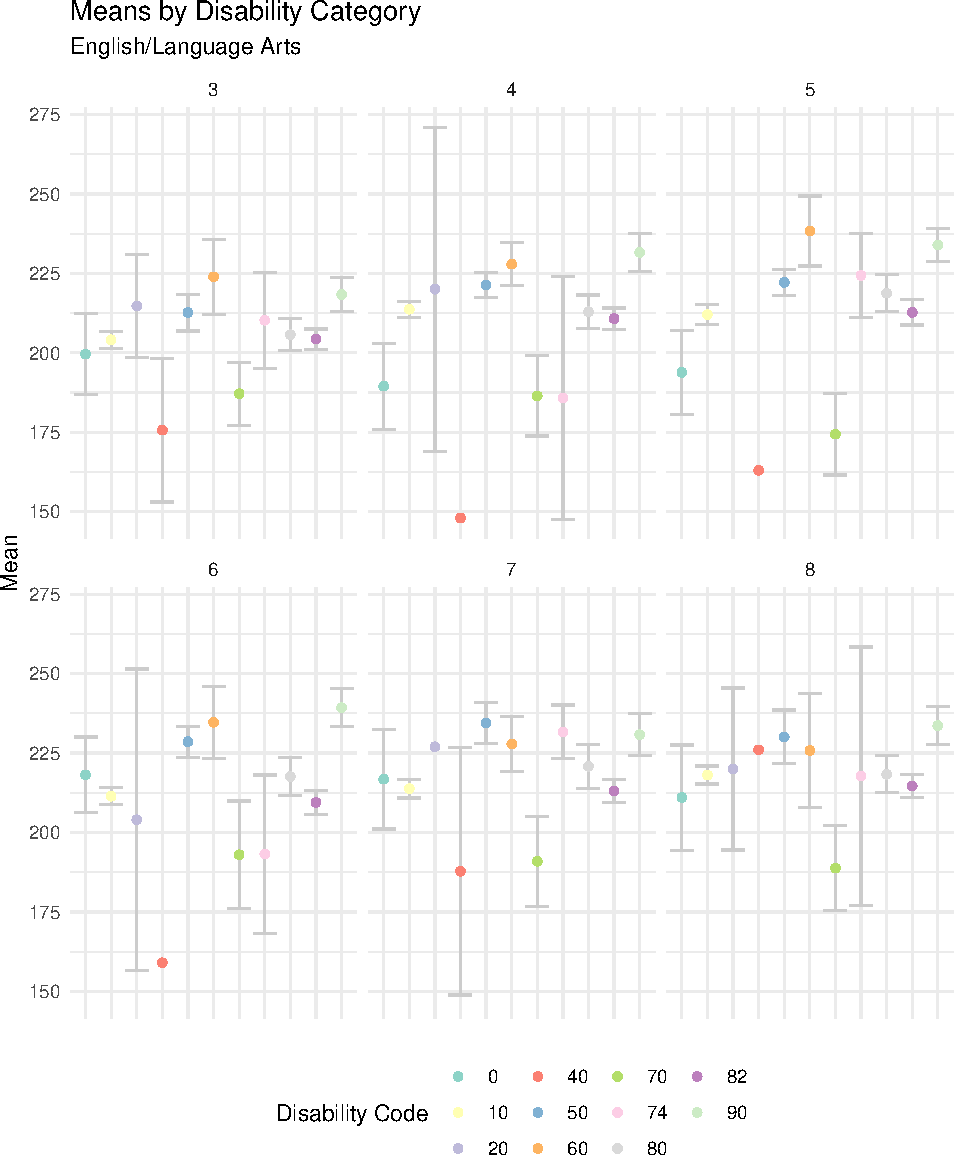
\includegraphics{tech_report_18_files/figure-latex/plots38-1.pdf}
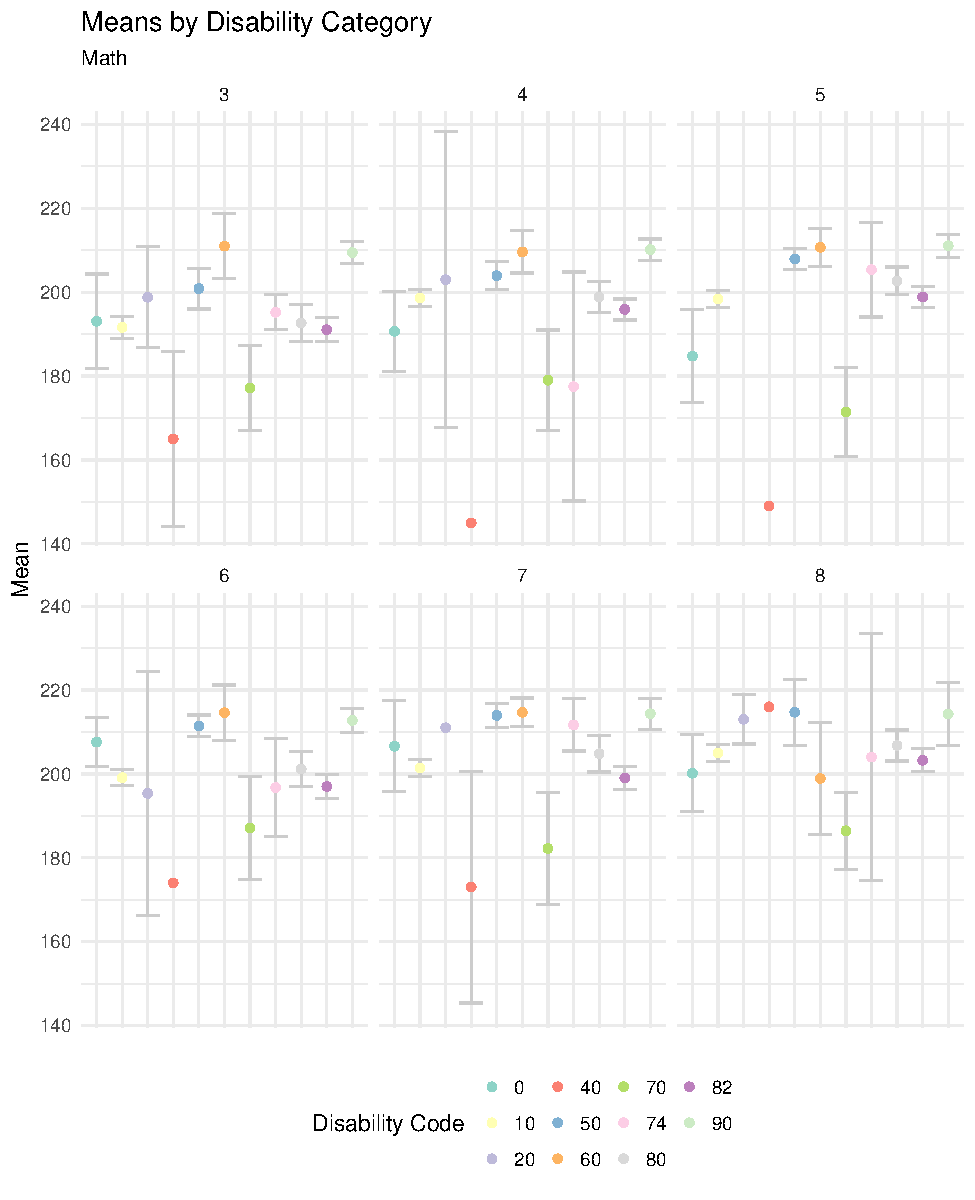
\includegraphics{tech_report_18_files/figure-latex/plots38-2.pdf}

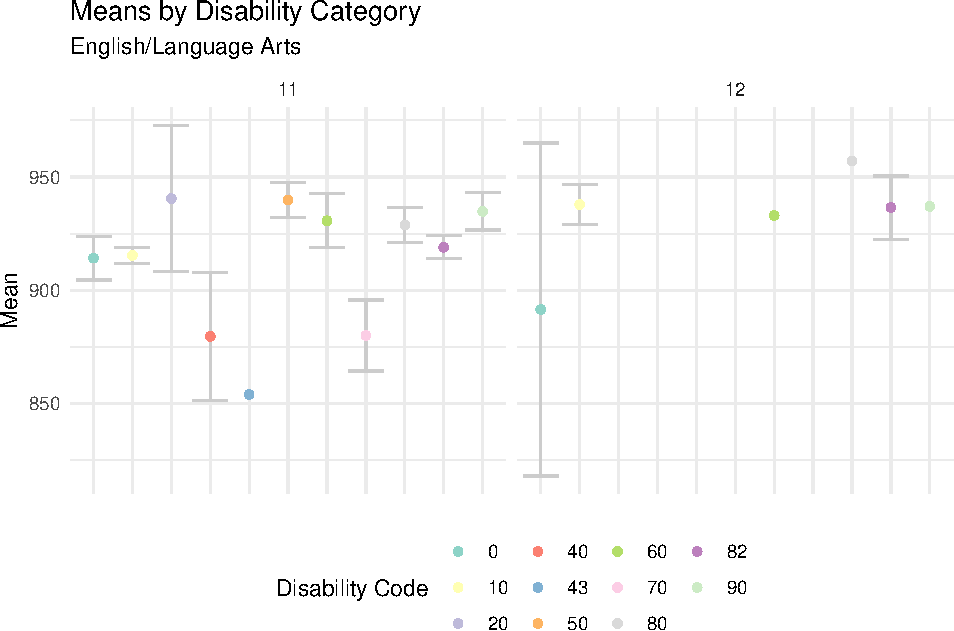
\includegraphics{tech_report_18_files/figure-latex/plots11-1.pdf}
\includegraphics{tech_report_18_files/figure-latex/plots11-2.pdf}

\includegraphics{tech_report_18_files/figure-latex/sci_plots5811-1.pdf}
\includegraphics{tech_report_18_files/figure-latex/sci_plots5811-2.pdf}
\includegraphics{tech_report_18_files/figure-latex/sci_plots5811-3.pdf}

\subsubsection{4.3 Full Performance
Continuum}\label{full-performance-continuum}

The ORExt is designed to sample the Common Core State Standards in
English language arts (Reading, Writing, and Language) and Mathematics,
as well as the Oregon Science Standards and Next Generation Science
Standards in science in a purposive, validated manner. The ORExt test
blueprints convey the balance of representation exhibited by the
assessment (see \emph{Appendix} 2.1B). These test blueprints are
supported by the \color{link}{[}ORExt Extended Assessment
Frameworks(\url{http://www.brtprojects.org/publications/training-modules})
\color{black}, which define the assessable content on the ORExt that has
been reduced in depth, breadth, and complexity (RDBC) using our defined
process (see \emph{Appendix} 2.3A.3). The decisions regarding which
standards to target for essentialization, as well as the strength of
linkage between the Essentialized Standards and the CCSS/ORSci/NGSS has
been validated by Oregon teachers, as well (see \emph{Appendix} 3.1A).

Though a simplified and standardized approach was taken to design items,
and efficiency and access to the assessment increased for the majority
of students (as evidenced by the decreased percentages of zero scores
across all content areas), a small subgroup of students remains who
cannot access an academic assessment. This is true even though items
have been significantly RDBC at three levels of complexity
(low-medium-high difficulty). As a response, ODE commissioned BRT to
design and implement an observational rating scale for this group of
very low-performing students, called the Oregon Observational Rating
Assessment (ORora) for the spring 2016 administration. The ORora targets
communication (expressive and receptive) and basic skills
(attention/joint attention and mathematics) and provides documentation
of student progress outside of our clearly defined academic domains.

Items on all assessments were scored on a 2-point scale, with 1 point
awarded for a correct response and 0 points awarded for an incorrect
response. Plots are provided below for each content area and grade
level, including the person ability and item difficulty distributions.
In general, the descriptive statistics suggest that the test had an
appropriate range of item difficulties represented, from easy to
difficult, with item difficulties generally ranging from -4.0 to +4.0 on
the Rasch scale. The assessments performed as expected across all grades
and content areas. The item person distributions provided below
demonstrate that the ORExt is providing a performance continuum for
students who participate.

\subsubsection{English Language Arts Person/Item
Distributions}\label{english-language-arts-personitem-distributions}

\begin{figure}
\centering
\includegraphics[height=4.16667in]{ipdens/ela3ipdens.pdf}
\caption{}
\end{figure}

\begin{figure}
\centering
\includegraphics[height=4.16667in]{ipdens/ela4ipdens.pdf}
\caption{}
\end{figure}

\begin{figure}
\centering
\includegraphics[height=4.16667in]{ipdens/ela5ipdens.pdf}
\caption{}
\end{figure}

\begin{figure}
\centering
\includegraphics[height=4.16667in]{ipdens/ela6ipdens.pdf}
\caption{}
\end{figure}

\begin{figure}
\centering
\includegraphics[height=4.16667in]{ipdens/ela7ipdens.pdf}
\caption{}
\end{figure}

\begin{figure}
\centering
\includegraphics[height=4.16667in]{ipdens/ela8ipdens.pdf}
\caption{}
\end{figure}

\begin{figure}
\centering
\includegraphics[height=4.16667in]{ipdens/ela11ipdens.pdf}
\caption{}
\end{figure}

\subsubsection{Mathematics Person/Item
Distributions}\label{mathematics-personitem-distributions}

\begin{figure}
\centering
\includegraphics[height=4.16667in]{ipdens/math3ipdens.pdf}
\caption{}
\end{figure}

\begin{figure}
\centering
\includegraphics[height=4.16667in]{ipdens/math4ipdens.pdf}
\caption{}
\end{figure}

\begin{figure}
\centering
\includegraphics[height=4.16667in]{ipdens/math5ipdens.pdf}
\caption{}
\end{figure}

\begin{figure}
\centering
\includegraphics[height=4.16667in]{ipdens/math6ipdens.pdf}
\caption{}
\end{figure}

\begin{figure}
\centering
\includegraphics[height=4.16667in]{ipdens/math7ipdens.pdf}
\caption{}
\end{figure}

\begin{figure}
\centering
\includegraphics[height=4.16667in]{ipdens/math8ipdens.pdf}
\caption{}
\end{figure}

\begin{figure}
\centering
\includegraphics[height=4.16667in]{ipdens/math11ipdens.pdf}
\caption{}
\end{figure}

\subsubsection{Science Person/Item
Distributions}\label{science-personitem-distributions}

\begin{figure}
\centering
\includegraphics[height=4.16667in]{ipdens/science5ipdens.pdf}
\caption{}
\end{figure}

\begin{figure}
\centering
\includegraphics[height=4.16667in]{ipdens/science8ipdens.pdf}
\caption{}
\end{figure}

\begin{figure}
\centering
\includegraphics[height=4.16667in]{ipdens/science11ipdens.pdf}
\caption{}
\end{figure}

\subsubsection{4.4 Scoring}\label{scoring}

All scoring expectations for the ORExt are established within the
Administration Manual (see \emph{Appendix} 2.3, p.~14). The scoring
procedures for the new ORExt have been simplified, with students
receiving a 0 for an incorrect response or a 1 for a correct response.
Input from the field gathered from Consequential Validity studies
demonstrates that the assessment scoring procedures are much more clear
and easier to implement than prior scoring approaches (see
\emph{Appendix} 2.3B.10). BRT was also commissioned to develop a scaled
score interpretation guide, which describes specific strategies for
interpreting student test scores and sub-test scores in Reading and
Writing, and Achievement Level Descriptors (ALDs) published within the
Individual Student Reports (see \emph{Appendix} 6.4C) for annual
performance, growth, and as part of Essential Skills requirements for
very low performing students (see \emph{Appendix} 2.1A).

\subsubsection{4.5 Multiple Assessment
Forms}\label{multiple-assessment-forms}

The ORExt was administered in only form per subject area and grade level
for the 2017-18 school year, with 36 operational items arranged in order
of empirical difficulty and 12 embedded field test items.

\subsubsection{4.6 Multiple Versions of An
Assessment}\label{multiple-versions-of-an-assessment}

The ORExt is provided in the standard format, but is also available in
Large Print and Brailled formats. Test content is identical across all
three versions, with an occasional item being eliminated on the Braille
version due to inaccessibility. These items do not count for or against
the student in reporting. Substantive test comparability analyses are
not feasible, given the small n-sizes of the samples involved in the
alternative versions.

\subsubsection{4.7 Technical Analyses and Ongoing
Maintenance}\label{technical-analyses-and-ongoing-maintenance}

The ORExt technical analyses that document reliability and validity are
included in this technical report (see Sections 3 and 4, respectively).
ODE and BRT staff review these analyses annually. Necessary adjustments
to the assessment are determined prior to implementation of the
subsequent year's work plan, which elaborates the areas of improvement
as well as aspects of the testing program that will be maintained. This
decision-making is supported by input from the field gathered from the
Consequential Validity study (see \emph{Appendix} 2.3B.10).

Within our system of ongoing improvement is continuation of the
development of additional curricular and instructional resources. This
addresses an area of concern expressed by stakeholders. Training modules
and templates continue to be developed to connect assessment results
from the ORExt and ORora with curricular resources and instructional
strategies aligned to the standards.

\subsection{Critical Element 5 - Inclusion of All
Students}\label{critical-element-5---inclusion-of-all-students}

\subsubsection{5.1 Procedures for Including
SWDs}\label{procedures-for-including-swds}

The Oregon assessment system provides explicit guidance regarding the
participation of all public school students in its statewide assessment
program (see Section 1.4).

\paragraph{5.1A Clear Explanations of the Differences Between
Assessments}\label{a-clear-explanations-of-the-differences-between-assessments}

The assessment options for all public school students in Oregon are
elaborated in the Oregon Test Administration Manual (see \emph{Appendix}
1.4.2, p.~7). These options include the Smarter Balanced Assessment in
English language arts and mathematics in Grades 3-8 \& 11, the Oregon
Assessment of Knowledge and Skills in science in Grades 5, 8, \& 11, and
in the same content areas and grade levels for SWSCD who take the ORExt
(see \emph{Appendix} 1.4.2, p.~92-93). Social studies assessment is a
district option within the OAKS portal, as well. In addition,
expectations for the English Language Proficiency Assessment (ELPA) and
the Kindergarten Assessment are provided.

\paragraph{5.1B Eligibility Decisions Made by IEP
Teams}\label{b-eligibility-decisions-made-by-iep-teams}

A student's IEP team determines how a student with disabilities will
participate in the Oregon Statewide Assessment program. The IEP team
must address the eligibility criteria for participation in the ORExt
before determining that the assessment is the appropriate option (see
\emph{Appendix} 5.1B).

\paragraph{5.1C Guidelines for Assessment
Selection}\label{c-guidelines-for-assessment-selection}

As noted earlier, IEP teams make decisions regarding how students with
disabilities participate in the Oregon statewide assessment program. At
present, students participate in one of three options: (a) student takes
the general assessment with or without universal tools. (b) student
takes the general assessment with designated supports and/or
accommodations, or (c) student takes the ORExt. Guidelines for making
universal support, designated support, and accommodations decisions for
the general assessments are provided in \emph{Appendix} 2.3A.1.
Guidelines for making these determinations for SWSCD who participate in
AA-AAAS are provided in \emph{Appendix} 5.1B.

\paragraph{5.1D Information on Accessibility
Options}\label{d-information-on-accessibility-options}

Information regarding accessibility options for the general assessment
can be found with the general assessment Peer Review evidence. For the
ORExt, accessibility is treated holistically, with universal design for
assessment concepts embedded in the item design and a wide variety of
accommodations also available if needed. Items are crafted to be
visually simple and clean. Graphic supports, which are always
black/white line drawings, are embedded in all items at the low level of
complexity but are phased out as items become more complex. Items are
designed to incorporate simplified language unless specific academic
vocabulary and concepts is what is being tested (see \emph{Appendix}
2.3A.3). The items on the ORExt are all selected response, with three
response options allowing for multiple modes of access (e.g., saying the
answer, pointing to the answer, eye gaze, switch, etc.). All text
presented to students is at least 18-pt font (larger, of course, in the
large print version). Sample items are presented in \emph{Appendix}
2.2.3. All accessibility supports, designated supports, and
accommodations for the ORExt are published in \emph{Appendix} 2.3A.1,
p.~36-43. For students who have very limited to no communication and are
unable to access even the most accessible items on the ORExt, an Oregon
Observational Rating Assessment (ORora) was implemented in 2015-16. The
ORora is completed by teachers and documents the student's level of
communication complexity (expressive and receptive), as well as level of
independence in the domains of attention/joint attention and
mathematics. The administration instructions and 2017-18 results for the
ORora are included in \emph{Appendix} 5.1D.

\paragraph{5.1E Guidance Regarding Appropriate
Accommodations}\label{e-guidance-regarding-appropriate-accommodations}

Guidance regarding appropriate accommodations is published in
\emph{Appendix} 2.3A.1. District and School Test Coordinators provide
annual training on test security and administration. The ORExt
approaches access as part of test design, as noted above in Section
5.1D. The complexity of SWSCD communication systems demands such an
approach. In addition, comprehensive accommodations are allowed in order
to decrease the chances that a disability may interfere with our ability
to measure the student's knowledge and skills.

\paragraph{5.1F All SWDs Eligible for the
ORExt}\label{f-all-swds-eligible-for-the-orext}

ODE's eligibility guidelines make it clear that all SWDs are eligible
for the ORExt, regardless of disability category, and that specific
disability category membership should not be a determining factor for
considering participation (see \emph{Appendix} 5.1B).

\paragraph{5.1G Parents Informed of AA-AAAS
Consequences}\label{g-parents-informed-of-aa-aaas-consequences}

The Parent FAQ section of the General Administration Manual makes it
clear that parents must be informed of the potential consequences of
having their child assessed against alternate achievement standards,
including diploma options. Parents are also informed that alternate
achievement standards are designed to reflect a significant reduction in
depth, breadth, and complexity and are therefore not comparable to
general academic achievement standards (see \emph{Appendix} 2.3,
p.~28-32).

\paragraph{5.1H State Ensures ORExt Promotes Access to the General
Education
Curriculum}\label{h-state-ensures-orext-promotes-access-to-the-general-education-curriculum}

The ORExt is strongly linked to the CCSS/ORSci/NGSS, as evidenced by our
linkage study results (see \emph{Appendix} 3.1A). The claim is based on
the following warrants: (a) ORExt items are aligned to the Essentialized
Standards; (b) the Essentialized Standards are strongly linked to the
grade level content standards; therefore (c) the ORExt items are
strongly linked to grade level content expectations. It is thus expected
that the ORExt promotes access to the general education curriculum by
assessing general education content that has been reduced in depth,
breadth, and complexity yet maintains the highest possible standard for
SWSCD.

In addition, ODE commissioned BRT to work with Oregon teachers of SWSCD
in the 2015-16 school year to develop a variety of curricular and
instructional resources that are aligned to the Essentialized Standards.
These resources include: (a) curricular templates, (b) video tutorials,
and (c) supporting documents that provide specific guidance regarding
how to develop lesson plans, Present Levels of Academic and Functional
Performance (PLAAFP) statements, and Individualized Education Program
(IEP) goals and objectives that are aligned with the Essentialized
Standards. It is also expected that the essentialization process will
generalize to many students who are performing off grade level, not
merely to SWSCD. All resources are published on a
\color{link}\href{http://lms.brtprojects.org}{BRT-sponsored
website}\color{black}.

\subsubsection{5.2A - 5.2C Procedures for Including
ELs}\label{a---5.2c-procedures-for-including-els}

In addition to the programmatic guidance provided in \emph{Appendix}
1.4A.1 related to EL program eligibility and services, ODE also provides
guidance relevant to the inclusion of ELs in the statewide assessment
program in \emph{Appendix} 1.4.2. Though the ORExt is currently
published in English, an appropriately qualified interpreter can provide
the assessment to any SWSCD from diverse language backgrounds, including
American Sign Language. ODE has developed a training module to increase
the standardization of \color{link}\href{http://lms.brtprojects.org}{ASL
administration} \color{black} for its statewide assessments.

Additional information regarding the inclusion of ELs in Oregon's
general assessments is provided in the general assessment Peer Review
evidence.

\subsubsection{5.3 Accommodations}\label{accommodations}

All statewide accommodation guidance is published in the Accessibility
Manual (see \emph{Appendix} 2.3A.1), outlining the universal tools and
designated supports available to all students, and accommodations,
available only to students with disabilities or students served by
Section 504 Plans. In addition, the manual defines the supports as
embedded, where they are provided by the online test engine (e.g.,
calculator, text-to-speech), or non-embedded, where they must be
provided by a qualified assessor (e.g., read aloud, scribe). The manual
also makes it clear that these supports are content-area specific, as a
universal tool in one content area may be an accommodation in another.

\paragraph{5.3A Appropriate Accommodations are Available for SWD/
Section
504}\label{a-appropriate-accommodations-are-available-for-swd-section-504}

Appropriate accommodations for the ORExt are published in
\emph{Appendix} 2.3A.1, p.~36-43. Additional accommodations for all
statewide assessments are also published in this manual. The Oregon
Accommodations Panel reviews the appropriateness of the supports listed
annually. Practitioners may also request the addition of an
accommodation through a formal process (see \emph{Appendix} E: Approval
Process for New Accessibility Supports within the manual,
\emph{Appendix} 2.3A.1, p.~100-102).

\paragraph{5.3B Appropriate Accommodations are Available for
ELs}\label{b-appropriate-accommodations-are-available-for-els}

As noted in Sections 5.2A-C, the ORExt is accessible in any
communication modality through the use of an interpreter. Appropriate
accommodations for the ORExt are published in \emph{Appendix} 2.3A.1,
p.~36-43. Additional accommodations for all statewide assessments are
also published in this manual. The Oregon Accommodations Panel reviews
the appropriateness of the supports listed annually. Practitioners may
also request the addition of an accommodation through a formal process
(see \emph{Appendix} E: Approval Process for New Accessibility Supports
within the manual, \emph{Appendix} 2.3A.1, p.~100-102).

\paragraph{5.3C Accommodations are Appropriate and
Effective}\label{c-accommodations-are-appropriate-and-effective}

In addition to the evidence gathered during the linkage study (see
\emph{Appendix} 3.1A), which suggests that the ORExt items were
accessible and free of bias even before final editing, the
appropriateness of the supports listed in \emph{Appendix} 2.3A.1 is
reviewed annually by the Oregon Accommodations Panel. Practitioners may
also request the addition of an accommodation through a formal process
(see \emph{Appendix} E: Approval Process for New Accessibility Supports
within the manual, \emph{Appendix} 2.3A.1, p.~100-102). ODE is
collecting accommodations codes for the ORExt from Qualified Assessors
who opt to enter this information in order to make performance
comparisons feasible. Accommodations information was collected in this
year's assessment. A study on the effect of the use of different
accommodations will be conducted and reported in the 2018-19 technical
report.

\paragraph{5.3D Accommodations are Appropriate and
Effective}\label{d-accommodations-are-appropriate-and-effective}

ODE has a formal process stakeholders can use to request accommodations
that are not already published in the Accessibility Manual (see
\emph{Appendix} E: Approval Process for New Accessibility Supports
within the manual, \emph{Appendix} 2.3A.1, p.~100-102).

\subsubsection{5.4A - 5.4E Monitoring Test Administration for Special
Populations}\label{a---5.4e-monitoring-test-administration-for-special-populations}

ODE monitoring of test administration in its districts and schools is
elaborated within the general assessment Peer Review evidence and is
therefore not addressed here.

\subsection{Critical Element 6 - Academic Achievement Standards and
reporting}\label{critical-element-6---academic-achievement-standards-and-reporting}

\subsubsection{6.1 State Adoption of Alternate Academic Achievement
Standards for
SWSCD}\label{state-adoption-of-alternate-academic-achievement-standards-for-swscd}

The Oregon Extended assessment (ORExt), Oregon's Alternate Assessment
based on Alternate Academic Achievement Standards (AA-AAAS), is part of
the Oregon Statewide Assessment System. The ORExt is administered to
Oregon students with the most significant cognitive disabilities (SWSCD)
in English language arts and mathematics in Grades 3-8 and 11. The ORExt
is administered in science in Grades 5, 8, \& 11. The ORExt links to the
CCSS in English language arts and mathematics. The new ORExt is dually
linked to Oregon's former science standards, as well as to the NGSS.
Results from the English language arts and math administrations are
included in calculations of participation and performance for Annual
Measurable Objectives (AMO) - a provision of the No Child Left Behind
Act (NCLB). Science participation is also included as part of the Title
1 Assessment System requirements, and is administered in grades 5, 8, \&
11.

The revised ORExt is built upon a vertical scale in order to support
reliable determinations of annual academic growth in ELA and mathematics
in Grades 3-8. The complete vertical scaling plan and operational item
selection decision rules are located in \emph{Appendix} 2.2.1.

\paragraph{6.1A State Formally Adopted Alternate Academic Achievement
Standards}\label{a-state-formally-adopted-alternate-academic-achievement-standards}

The State Board of Education formally adopted the AAAS and achievement
level descriptors (ALDs) on June 25, 2015 (see \emph{Appendix} 6.1A.1).
The ELA, Math, and Science AAAS, including both the ALDs and the
requisite cut scores are included in \emph{Appendix} 6.1.A.2.

\paragraph{6.1B State Applies AAAS to All Public School SWSCD in Tested
Grades}\label{b-state-applies-aaas-to-all-public-school-swscd-in-tested-grades}

The state applies the AAAS to all public school-served SWSCD who
participate in the ORExt in Grades 3-8 \& 11 in English language arts
and mathematics, and in Grades 5, 8, \& 11 in science.

\paragraph{6.1C State's AAAS Include At Least Three Levels, ALDs, and
Cut
Scores}\label{c-states-aaas-include-at-least-three-levels-alds-and-cut-scores}

The alternate academic achievement standards in Oregon are composed of
four levels (though only three are required). In descending order, they
are (a) Level 1, (b) Level 2, (c) Level 3, and (d) Level 4. Level 1 and
Level 2 performances represent proficient achievement, while the bottom
two levels represent achievement that is not yet proficient. The
procedures followed to develop Oregon's alternate academic achievement
standards were consistent with Title 1 assessment system requirements,
including the establishment of cut scores, where relevant. In order to
define four levels of proficiency, Oregon set three cut scores across
all subject areas: (a) to separate Level 1 from Level 2, (b) to separate
Level 2 from Level 3, and, (c) to separate Level 3 from Level 4. The
alternate academic achievement standards in English language arts,
mathematics, and science for the ORExt, including the achievement level
descriptors (ALDs) and cut scores, were established during standard
setting meetings held on June 15 (science), 16 (mathematics), and 17
(English language arts).

\subsubsection{6.2 Achievement Standard
Setting}\label{achievement-standard-setting}

Standard Setting meetings were held at the University of Oregon in
Eugene, OR on June 15, 2015 (Science), June 16, 2015 (Mathematics), and
June 17, 2015 (English language arts). A total of 53 standard setters
were involved in the process: 11 in Science, and 21 in both English
language arts and Mathematics. Panelists were assembled in grade level
teams of three, where two members were special educators and one member
was a content specialist.

The panelists were highly educated. Over 90\% of the panel possessed a
Master's degree or higher. Fifty-seven (57\%) percent of the panelists
had over 11 years of teaching experience. Seventy-six percent (76\%) of
the panelists had some experience working with students with significant
cognitive disabilities with 64\% licensed as Special Educators. The
majority of panel members were female (87\%), from the Northwest of the
state (87\%), and White (83\%). No panel member self-identified with
Oregon's major minority population (Hispanic).

In addition to the live training during standard setting meetings,
panelists were asked to complete several training requirements prior to
the standard setting meetings, which oriented them to the student
population of students with significant cognitive disabilities (SWSCDs),
the Oregon Extended Assessment test design and history, as well as the
bookmarking standard setting method. Panelists were quite confident in
their preparation and final judgments, as evidenced by responses to the
questions: (a) " The training helped me understand the bookmark method
and how to perform my role as a standard setter." (b) ``I am confident
about the defensibility and appropriateness of the final recommended cut
scores.'' and, (c) ``Overall, I am confident that the standard setting
procedures allowed me to use my experience and expertise to recommend
cut scores for the ORExt.'' The hearty majority of standard setters
strongly agreed with these statements, while all participants agreed.

The nine-step process implemented for these standard setting meetings
was based on Hambleton \& Pitoniak (2006) as reported by R.L. Brennan
(Educational Measurement, 4th Edition, pp.~433-470). Standard setting
evaluation questions posed to participants were adapted from Cizek's
Setting Performance Standards (2012). Standard setters set cut scores
and recommended Achievement Level Descriptors (ALDs) for the Oregon
State Board of Education to consider. The cut scores were articulated to
reflect vertical development, or at least maintenance, of expectations
across grades in a manner that respected standard setter judgments to
the greatest possible degree. Six changes were made in ELA and
Mathematics. Science is not built upon a vertical scale, so no cut score
adjustments were necessary in Science. The cut scores are listed below.

English language arts (ELA) table here:

Mathematics table here:

Science table here:

Note: The ELA and Math vertical scales for the ORExt are centered on 200
in grades 3-8 and can be used to document year-to-year growth. None of
the other scales should be used for longitudinal comparisons. All Grade
11 scales are independent and centered on 900. The grade 5 Science scale
is independent and centered on 500, while the Grade 8 Science scale is
independent and centered on 800. An independent auditor evaluated the
bookmarking standard setting process. The auditor's comprehensive report
can be found in \emph{Appendix} 6.2.2.

\subsubsection{6.3 Challenging and Aligned Academic Achievement
Standards}\label{challenging-and-aligned-academic-achievement-standards}

Oregon educators initially evaluated new Oregon Essentialized Assessment
Frameworks in two respects. First, educators were asked to determine the
appropriateness of the standards selected for inclusion and exclusion in
the Essentialized Standards (yes/no). Second, the level of linkage
between the Essentialized Standards and grade level content standard was
evaluated (0 = no link, 1 = sufficient link, 2 = strong link). Summary
results are provided in the tables below. A comprehensive essentialized
standard to grade level standard linkage study, as well as essentialized
standard to item alignment study, is provided in \emph{Appendix} 3.1A.

English language arts table here:

Mathematics table here:

Science table here:

\subsubsection{6.4 Reporting}\label{reporting}

Oregon's reporting system facilitates appropriate, credible, and
defensible interpretation and use of its assessment data. With regard to
the ORExt, the purpose is to provide the state technically adequate
student performance data to ascertain proficiency on grade level state
content standards for students with significant cognitive disabilities
(see Sections 3 and 4). In addition, the state makes it clear that
results from the Oregon Extended are not comparable to results from the
SBA/OAKS (see \emph{Appendix} 2.3, p.~29-31). Nevertheless, the test
meets rigorous reliability expectations (see Section 4.1). Validity is
considered here as an overarching summation of the Oregon Extended
assessment system, as well as the mechanisms that Oregon uses to
continuously improve the ORExt assessment (see \emph{Appendix} 2.3B.10).

\paragraph{6.4A Public Reporting}\label{a-public-reporting}

Oregon reports participation and assessment results for all students and
for each of the required subgroups in its reports at the school,
district, and state levels. The state does not report subgroup results
when these results would reveal personally identifiable information
about an individual student. The calculation rule followed is that the
number of students in the subgroup must meet the minimum cell size
requirement for each AMO decision: participation, achievement in English
language arts and math, attendance, and graduation, where appropriate
(see \emph{Appendix} 2.6C).

\paragraph{6.4B State Reports Interpretable
Results}\label{b-state-reports-interpretable-results}

Oregon develops and disseminates individual student data upon final
determination of accuracy. The state provides districts with individual
student reports (ISRs) that meet most relevant requirements. The state
incorporated the Standard Error of Measure (SEM) for each student score
into the report templates. The SEM associated with each cut score is
provided in Section 4.1B. Also, see the mock-up ISR in \emph{Appendix}
6.4C.

\paragraph{6.4C1 - C5 State Provides Individual Student
Reports}\label{c1---c5-state-provides-individual-student-reports}

Oregon's student reports provide valid and reliable information
regarding achievement on the assessments relative to the AAS. The
reliability of the data is addressed in Section 4.1. Validity is
considered here as an overarching summation of the Oregon Extended
assessment system, as well as the mechanisms that Oregon uses to
continuously improve the Oregon Extended assessment. The ISRs clearly
demonstrate the students' scale score relative the AAAS that is relevant
for that content area and grade level (see Section 4.4 and
\emph{Appendix} 6.4C). The Oregon ISRs provide information for parents,
teachers, and administrators to help them understand and address a
student's academic needs. These reports are displayed in a simple format
that is easy for stakeholders to understand. District representatives
can translate results for parents as necessary. Scaled score
interpretation guidance is published in \emph{Appendix} 2.1A.

\subsection{Conclusions and Next
Steps}\label{conclusions-and-next-steps}

In sum, the rigor of the procedural development and statistical outcomes
of the ORExt were substantive and support the assessments intended
purpose. Procedural evidence includes essentialized standards
development, item development, item content and bias reviews, an
independent alignment study and item selection based upon item
characteristics. Outcome-related evidence included measure reliability
analyses, point measure biserials, outfit mean squares, item difficulty
and person ability distributions, and convergent and divergent validity
evidence. These sources of evidence were all quite good and provide
important validity evidence.

The test development process adhered to procedural guidelines defined by
the AERA/APA/NCME Standards for Educational and Psychological Testing
(2014), as well as incorporating procedures that are known in the field
to be best practice. For example, an independent auditor evaluated
alignment. In addition, the ORExt reflects what highly qualified Oregon
educators believe represents the highest professional standards for the
population of students with significant cognitive disabilities, as
evidenced in our consequential validity study by teacher support of the
academic content on the ORExt as well as the behaviors sampled during
test administration.

Dr.~Dianna Carrizales conducted an independent alignment study
consisting of five evaluation components: a) standard selection for
essentialization, b) strength of linkage between essentialized standards
and grade level content standards, c) alignment between items and
essentialized standards, d) alignment between the essentialized
standards and the achievement level descriptors, and e) alignment
between the achievement level descriptors and the ORExt test items.
Dr.~Carrizales reported that, ``In the three evaluations that involved
determining the relationship between standards and items, reviewers
identified sufficient to strong relationships among assessment
components in all grades and all subject areas. In the two evaluations
involving Achievement Level Descriptors, reviewers identified thirty
instances of sufficient to strong relationships out of thirty-four
possible relationship opportunities resulting in an overall affirmed
relationship with areas for refinements identified.'' Overall,
documentation collected in the report suggests that the ORExt assessment
system is aligned.

The test reliabilities for the ORExt were quite high, suggesting that
the assessment items functioned consistently with the test as a whole.
The correlations between students' content scores across subjects were
not overly strong, implying that each test measures a distinct
construct. The classification consistency analyses demonstrate that the
ORExt is appropriately categorizing students into the proficient
category, and capable of doing so in a consistent manner. The vertical
scale developed in 2014-15 appears to be modeling incremental growth
across Grades 3-8 in ELA and mathematics, as intended. The Grade 7
mathematics test continued to demonstrate insufficient item difficulties
across the range of low, medium, and high item complexity, however, and
must again be amended in the 2017-18 school year. The ELA and science
assessments could continue to benefit from the addition of more
difficult items, as evidenced by comparisons of the average person
abilities and item difficulties. Mathematics assessments appear to be
functioning quite well in terms of person abilities and item
difficulties, though some additional low level items might help increase
access for the group of students functioning at that level.

The Oregon Observational Rating Assessment (ORora) results demonstrate
that approximately 17-25\% of the SWSCD who participated in the ORExt
also took the ORora, depending upon grade level. A total of 755 students
were administered the ORora in the 2016-17 test administration. The
participants were primarily students with multiple, severe disabilities
with very limited communication systems. Analyses of missing data
patterns for the ORExt demonstrated that QAs were generally able to
adhere to the discontinuation rules. Quantitative results indicate that
a total of 755 students across all tested grades were administered the
ORora. Response patterns on the ORExt were compared to ORora results to
determine what percentages of QAs were administering the ORora due to
the minimum participation rule and what percentage were administering
the ORora of their own volition. Analyses showed that 234 students were
eligible to take the ORora in English language arts, 241 students were
eligible to take the ORora in mathematics, and 86 were eligible to take
the ORora in science. This means that about 30 students per grade, per
content area received five or fewer correct responses within the first
15 items administered on the ORExt. Of the 561 test records that met
ORora eligibility requirements, 91 were not administered the ORora. In
addition, there were 82 students in ELA and Math, respectively, who were
administered the ORora without having participated in the ORExt (74 of
those students were the same students, across each content area, with
eight students unique to each content area, respectively).

The 2016-17 Oregon Consequential Validity study provides important
information for future administrations of the ORExt. The results
demonstrate that the test continues to be easy to administer and score
and is providing an accessible and appropriate representation of the
knowledge and skills that should be required of SWSCD in Oregon. Areas
of requested improvement include the provision of a tablet-based
administration, which is already planned for 2017-18, and the
development of additional life skills items, which cannot be
accomplished while maintaining rigorous academic expectations that are
linked to Oregon content standards.

The 2016-17 Oregon Extended Assessment Pilot Tablet Administration
demonstrated that Oregon teachers highly value provision of a
tablet-based administration of the ORExt at the statewide level.
Benefits of a tablet-based administration included: increased student
engagement, improved standardization, ease of use by teachers, and
resource protection (i.e., time, printing, expense). The results also
suggest that more robust systems are needed to support user access to
the testing application via an automatic username and password process.
Focus Group members also recommended that practice items be developed in
a tablet format so qualified assessors and students can practice with
the tablet administration in preparation for the ORExt test window.

Documenting evidence of validity remains an ongoing and continuous
process. Our efforts to continue to improve the assessment system are
outlined below, as well as in Sections 3 and 4 above. We also have
studies planned over the course of the next three years that will help
to solidify the evidence that is accumulating. All of the evidence we
have at hand suggests that the ORExt is sufficient to its stated purpose
of providing reliable determinations of student proficiency at the test
level in order to support systems level analysis of district and state
programs. The ORExt will hopefully continue to improve over time due to
field-testing and constant monitoring and review, and additional
validity evidence will be gathered.

As mentioned above in Section 3.1A, data are presented to support the
claim that Oregon's AA-AAAS provides the state technically adequate
student performance data to ascertain proficiency on grade level state
content standards for students with significant cognitive disabilities -
which is its defined purpose. In this technical report, we have provided
content validity evidence related to the ORExt test development process
(i.e., essentialization process, linkage study, distributed item review,
test blueprint, item writer training and demographics, and item reviewer
training and demographics), ORExt test reliability evidence, and ORExt
consequential validity evidence. Further analyses over the coming years
are planned to continue the development of technical documentation for
overall construct validity of the ORExt. The technical documentation
plan for the 2016 through 2019 school years is provided below:

Technical documentation plan for the 2016 through 2019 table here:

\subsection{Appendix Descriptions}\label{appendix-descriptions}

\paragraph{Appendix 1.1}\label{appendix-1.1}

\emph{Appendix} 1.1 explains the development process and intended uses
for the Essentialized Assessment Frameworks (EAFs). The EAFs are the
essentialized standards (EsSt), which are linked to grade level content
standards. The ORExt is aligned to the EAFs, as well. While the EAFs
primarily guide item development, they are also intended to be used in
the development of appropriate Present Levels of Functional and Academic
Performance (PLAAFP) statements and Individualized Education Program
(IEP) goals and objectives.

\paragraph{Appendix 1.2}\label{appendix-1.2}

\emph{Appendix} 1.2 conveys the evaluation conducted by researchers at
the Fordham Institute, which compared then-current state standards to
the CCSS in terms of rigor. The findings generally show that the CCSS
are as rigorous or more rigorous than state standards.

\paragraph{Appendix 1.4.1}\label{appendix-1.4.1}

\emph{Appendix} 1.4.1 is the Executive Memo from the Governor of Oregon
regarding parent opt-out expectations.

\paragraph{Appendix 1.4.2}\label{appendix-1.4.2}

\emph{Appendix} 1.4.2 is the test administration manual (TAM) for all
assessments in the Oregon statewide assessment system, including the
SBA, OAKS, the ORExt, the Kindergarten Assessment, and the ELPA. The TAM
elaborates all relevant test security and administration procedures.

\paragraph{Appendix 1.4A.1}\label{appendix-1.4a.1}

\emph{Appendix} 1.4A.1 is ODE's English Learner Program Guide, outlining
English learner (EL) system requirements in the areas of student
identification, services, reporting, and assessment for ELs in Oregon's
public schools, including ELs who are SWD.

\paragraph{Appendix 1.4A.2}\label{appendix-1.4a.2}

\emph{Appendix} 1.4A.2 is Oregon's regulations that require ODE to
provide translated OAKS assessments for populations at or above 9\% in
grades K-12 within three years after the school year in which the
language exceeds the threshold.

\paragraph{Appendix 1.5}\label{appendix-1.5}

\emph{Appendix} 1.5 is Oregon's annual report to the state legislature
for the 2015-16 school year. The report includes student demographics
and information on student groups, school funding and staff information,
test results, graduation and drop out rates, charter school data and
information on alternative education programs, early childhood data, and
attendance and chronic absenteeism data.

\paragraph{Appendix 2.1}\label{appendix-2.1}

\emph{Appendix} 2.1 is the test specifications document that describes
our approach to assessment and test design for the ORExt. The document
includes our approach to RDBC, an overview of the essentialization
process and EAF documents, the anticipated operational test design for
the ORExt, test development considerations, sample test items, item
specifications, and universal tools/designated supports/accommodations.

\paragraph{Appendix 2.1A}\label{appendix-2.1a}

\emph{Appendix} 2.1A provides the field with comprehensive information
related to scaled score interpretation for the ORExt. The guidance is
published in three main areas: 1) Annual performance, 2) Annual growth,
and 3) Performance for very low functioning students. Guidance regarding
use and interpretation of reading and writing subscores is also
provided.

\paragraph{Appendix 2.1B}\label{appendix-2.1b}

\emph{Appendix} 2.1B is the test blueprint for the ORExt, conveying the
balance of representation of domains across the content areas and grade
levels assessed. Operational items are selected to reflect the
representation percentages included in the test blueprint.

\paragraph{Appendix 2.1C}\label{appendix-2.1c}

\emph{Appendix} 2.1C describes the eight-step item development process
used to develop items for the ORExt, from standard selection to test
booklet formation. The item development process is specific and explicit
in order to increase transparency.

\paragraph{Appendix 2.2.1}\label{appendix-2.2.1}

\emph{Appendix} 2.2.1 is the set of PPT slides that were used to train
item writers for the ORExt. Item writers were also provided an
orientation to the test specifications as part of training.

\paragraph{Appendix 2.2.2}\label{appendix-2.2.2}

\emph{Appendix} 2.2.2 is a document that summarizes the balanced design
vertical scaling plan employed for the ORExt in the 2014-15
administration. The document includes the domain sampling plan for all
assessments, as well as the decision rules employed to remove items from
the operational item pool prior to vertical scaling and standard setting
procedures.

\paragraph{Appendix 2.2.3}\label{appendix-2.2.3}

\emph{Appendix} 2.2.3 provides stakeholders with visual representation
of the structure of the ORExt. Sample items are conveyed in English
language arts, mathematics, and science, with the scoring protocol and
student materials presented together. Stakeholders can see the structure
of each item, as well as how the items are scored. They can also gather
an idea about the types of formats that are used for answer choices that
are included within the student materials documents.

\paragraph{Appendix 2.3}\label{appendix-2.3}

\emph{Appendix} 2.3 is ODE's General Administration and Scoring Manual
for 2017-18. The manual establishes ODE's expectations regarding the
test window, utilizing the ORExt training and proficiency website, using
the sign language interpreter training and proficiency website, and
informing parents. It also provides the following information for
stakeholders, including educators and parents: " Overview of the
Extended Assessments " Assessing a Student " Scoring " Decision Making "
Information for Teachers The manual provides three appendices that
provide guidance regarding the provision of supports, parent questions
and answers, and a glossary.

\paragraph{Appendix 2.3A.1}\label{appendix-2.3a.1}

\emph{Appendix} 2.3A.1 is the 2017-18 accessibility options manual for
all assessments in the Oregon statewide assessment system, including the
SBA, OAKS, the ORExt, and the ELPA. Options include Universal Tools,
Designated Supports, and Accommodations. The manual provides guidance
regarding use of these options in instruction and assessment, as well as
implementation strategies and use evaluation. Each accommodation is
coded for use in data analysis related to assessment scores for the SBA
and OAKS.

\paragraph{Appendix 2.3A.2}\label{appendix-2.3a.2}

\emph{Appendix} 2.3A.2 is ODE's How to Select, Administer, and Evaluate
Accommodations on Oregon's Statewide Assessment manual for 2013-14. The
manual trains users regarding how to implement and evaluate appropriate
accommodations, from the student level to the systems level.

\paragraph{Appendix 2.3A.3}\label{appendix-2.3a.3}

\emph{Appendix} 2.3A.3 is a document that summarizes the procedures used
during item development to reduce item depth, breadth, and complexity,
in addition to the test specifications information found in
\emph{Appendix} 2.1. The document also provides more detail regarding
how language complexity is addressed and reviewed in an effort to
decrease the language load of items and make the test more accessible to
all students. The document also discusses ways in which bias is
addressed during test development.

\paragraph{Appendices 2.3B.1-2.3B.2}\label{appendices-2.3b.1-2.3b.2}

Appendices 2.3B.1 and 2.3B.2 are the PowerPoint (PPT) trainings that
were used by ODE and BRT trainers to train new qualified assessors (QAs)
and qualified trainers (QTs) in four regionally hosted trainings in
November 2017. QTs also used the package to train New Qualified
Assessors for the 2017-18 school year. The training provides
participants with the information needed to pass proficiency tests as
part of the requirements to become a QA for the Oregon Extended
Assessments and was delivered by QTs throughout the state. The training
package addresses the following topics: ``What's new in 2017-18?'',
``2018 Test Window'', ``Eligibility - which students take AA-AAAS?'',
``Test administration'', ``Student Confidentiality \& Test Security'',
``Test Administration (Physical \& Logistic)'', ``Scoring \& Data
Entry'', ``Reports \& Sharing Results with Parents'', ``Navigating the
Training and Proficiency website'', and ``Resources.''

\paragraph{Appendix 2.3B.4}\label{appendix-2.3b.4}

\emph{Appendix} 2.3B.4 is the test calendar for the entire Oregon
statewide assessment program, including the SBA, OAKS, the ORExt, the
ELPA, the Kindergarten Assessment, and the NAEP.

\paragraph{Appendix 2.3B.5}\label{appendix-2.3b.5}

\emph{Appendix} 2.3B.5 is a sample agenda that ODE makes available to
QTs around the state to train their respective new QAs as they implement
the train-the-trainers model used by the Oregon Extended assessment.

\paragraph{Appendix 2.3B.6}\label{appendix-2.3b.6}

\emph{Appendix} 2.3B.6 is the list of instructions provided to new QAs
and QTs regarding how to access the online training and proficiency
website.

\paragraph{Appendix 2.3B.7}\label{appendix-2.3b.7}

\emph{Appendix} 2.3B.7 is the list of responsibilities associated with
being a QT for the ORExt assessment.

\paragraph{Appendix 2.3B.8}\label{appendix-2.3b.8}

\emph{Appendix} 2.3B.8 is the document that contains the most commonly
fielded questions and answers from stakeholders, including parents and
teachers.

\paragraph{Appendix 2.3B.9}\label{appendix-2.3b.9}

\emph{Appendix} 2.3B.9 is the Helpdesk log report that summarizes all of
the technical assistance questions garnered from the field this year.
Efforts are made to find any patterns that our team may use to improve
training for the following year.

\paragraph{Appendix 2.3B.10}\label{appendix-2.3b.10}

\emph{Appendix} 2.3B.10 is the consequential validity report for the
spring 2017 consequential validity study conducted by BRT. The report
provides documentation of the perceptions in the field related to both
intended and unintended academic and social consequences of the ORExt.

\paragraph{Appendices 2.6}\label{appendices-2.6}

\emph{Appendix} 2.6 is the data entry guide. The guide explains the
paper/pencil data entry process located on ODE's secure server. {]}

\paragraph{Appendices 2.6A}\label{appendices-2.6a}

\emph{Appendix} 2.6A is the ORExt Test Application User Guide. With
2017-18 the first year the tablet/web-based platform was available for
all grade level and subject area tests, this guide walked through the
system requirements, download/login instructions, testing process, and
troubleshooting.

\paragraph{Appendix 2.6C}\label{appendix-2.6c}

\emph{Appendix} 2.6C is the manual defining the state of Oregon's
policies and procedures regarding how students are included in AMO
reporting, including how achievement, growth, and graduation rates are
reported for student groups and subgroups.

\paragraph{Appendix 3.1A}\label{appendix-3.1a}

\emph{Appendix} 3.1A is a document that summarizes the independent
alignment study process and participants used to review the linkage
between the Essentialized Standards and grade level content standards
(CCSS in ELA and Math; ORSci and NGSS in Science), as well as the
alignment between test items for the ORExt with those Essentialized
Standards. In addition, reviewers rated the items for potential bias and
access concerns. All data was gathered using the Distributed Item Review
(DIR) website, supported by a webinar training and ongoing technical
assistance. The results of the 2014-15 Linkage Study, which was not
independent but run by BRT researchers, are also included.

\paragraph{Appendix 3.1B}\label{appendix-3.1b}

\emph{Appendix} 3.1B is a document that describes the Distributed Item
Review (DIR) website used by Oregon teachers to evaluate the alignment
between test items for the ORExt with Essentialized Standards. In
addition, reviewers rated the items for potential bias and access
concerns. All data was gathered using the DIR website, supported by a
webinar training and ongoing technical assistance.

\paragraph{Appendices 4.1}\label{appendices-4.1}

\emph{Appendix} 4.1 is the Inter-rater Reliability Study Observation
form completed by study participants.

\paragraph{Appendix 4.1B}\label{appendix-4.1b}

\emph{Appendix} 4.1B conveys the historical development of the ORExt
from 1999 to the present, including the grade levels/bands assessed,
content areas assessed, and the targeted content standards.

\paragraph{Appendix 4.2}\label{appendix-4.2}

\emph{Appendix} 4.2 includes the most current published state level data
regarding Oregon's ethnic diversity.

\paragraph{Appendix 5.1B}\label{appendix-5.1b}

\emph{Appendix} 5.1B is the revised and rigorous guidance that ODE has
provided to IEP teams to assist them in making appropriate assessment
eligibility determinations for students with disabilities.

\paragraph{Appendix 5.1D}\label{appendix-5.1d}

\emph{Appendix} 5.1D includes a summary report of the statewide results
and the administration and scoring instructions for the new Oregon
Observational Rating Assessment (ORora). The ORora is administered to
all students whose ORExt testing was discontinued. It provides
information regarding student progress in terms of functional skills in
adaptive and communication domains for the small subgroup of students
who are unable to meet the academic expectations in the ORExt.

\paragraph{Appendix 6.1A.1}\label{appendix-6.1a.1}

\emph{Appendix} 6.1A.1 is the agenda and minutes that document the
hearing and adoption of the AAAS for the ORExt on June 25, 2015.

\paragraph{Appendix 6.1A.2}\label{appendix-6.1a.2}

\emph{Appendix} 6.1A.2 includes all of the achievement level descriptors
(ALDs) and cutscores that define performance for the ORExt in
qualitative and quantitative fashions, respectively. These Alternate
Academic Achievement Standards (AAAS) describe what students should know
and be able to do based upon their performance on the ORExt.

\paragraph{Appendix 6.2.1}\label{appendix-6.2.1}

\emph{Appendix} 6.2.1 is the PPT slides used to train standard setters
during the June 2015 standard setting meetings for ELA, math, and
science.

\paragraph{Appendix 6.2.2}\label{appendix-6.2.2}

\emph{Appendix} 6.2.2 is a standard setting report generated by an
independent auditor. The report provides a comprehensive evaluation of
the bookmark standard setting procedure employed for the ORExt on June
15-17, 2015.

\paragraph{Appendix 6.4C}\label{appendix-6.4c}

\emph{Appendix} 6.4C is a document that displays the individual student
report (ISR) that ODE publishes for students who participate in the
ORExt. The mock-up includes cut scores and achievement level descriptors
(ALDs), as well as links to the ODE website for additional information.

\newpage

\section{References}\label{references}


\end{document}
